\documentclass[12pt]{book}
% Christian Bagshaw, Lauren DeDieu, Kimberly Golubeva, and Jerrod M.~Smith 
% A Resource Bank for Writing Intensive Mathematics Courses
% This work is licensed under a  Creative Commons Attribution-NonCommercial-ShareAlike 4.0 International License
% http://creativecommons.org/licenses/by-nc-sa/4.0/
\usepackage[framemethod=TikZ]{mdframed}
\usepackage{amsthm}
\usepackage{amsmath}
\usepackage{amssymb}
\usepackage{verbatim} %% for command \begin{comment} \end{comment}
\usepackage{bm} % bold math
\usepackage{mathtools}
\usepackage{xcolor} % to define colours
\usepackage{todonotes}
\usepackage{pdfpages} %% including whole pages pdf files
\usepackage{multicol}
%\usepackage{draftwatermark}
%	\SetWatermarkText{Draft. Date.}
%	\SetWatermarkScale{4}
\usepackage[pdftex,colorlinks,linktocpage=true,citecolor=blue,linkcolor=magenta]{hyperref} 
%%%%%%%%%%%%%%%%%%%%%%%%%%%%%%
%		Coloured Box Environments
%%%%%%%%%%%%%%%%%%%%%%%%%%%%%%
% Theorem
\newcounter{thm}[section] \setcounter{thm}{0}
\renewcommand{\thethm}{\arabic{chapter}.\arabic{section}.\arabic{thm}}
\newenvironment{thm}[2][]{%
\refstepcounter{thm}%
\ifstrempty{#1}%
{\mdfsetup{%
frametitle={%
\tikz[baseline=(current bounding box.east),outer sep=0pt]
\node[anchor=east,rectangle,fill=cyan!30]
{\strut Theorem~\thethm};}}
}%
{\mdfsetup{%
frametitle={%
\tikz[baseline=(current bounding box.east),outer sep=0pt]
\node[anchor=east,rectangle,fill=cyan!30]
{\strut Theorem~\thethm:~#1};}}%
}%
\mdfsetup{innertopmargin=10pt,linecolor=cyan!30,%
linewidth=2pt,topline=true,%
frametitleaboveskip=\dimexpr-\ht\strutbox\relax
}
\begin{mdframed}[]\relax%
\label{#2}}{\end{mdframed}}
%%%%%%%%%%%%%%%%%%%%%%%%%%%%%%
% Lemma
\newenvironment{lem}[2][]{%
\refstepcounter{thm}%
\ifstrempty{#1}%
{\mdfsetup{%
frametitle={%
\tikz[baseline=(current bounding box.east),outer sep=0pt]
\node[anchor=east,rectangle,fill=olive!30]
{\strut Lemma~\thethm};}}
}%
{\mdfsetup{%
frametitle={%
\tikz[baseline=(current bounding box.east),outer sep=0pt]
\node[anchor=east,rectangle,fill=olive!30]
{\strut Lemma~\thethm:~#1};}}%
}%
\mdfsetup{innertopmargin=10pt,linecolor=olive!30,%
linewidth=2pt,topline=true,%
frametitleaboveskip=\dimexpr-\ht\strutbox\relax
}
\begin{mdframed}[]\relax%
\label{#2}}{\end{mdframed}}
%%%%%%%%%%%%%%%%%%%%%%%%%%%%%%
% Corollary
\newenvironment{cor}[2][]{%
\refstepcounter{thm}%
\ifstrempty{#1}%
{\mdfsetup{%
frametitle={%
\tikz[baseline=(current bounding box.east),outer sep=0pt]
\node[anchor=east,rectangle,fill=violet!30]
{\strut Corollary~\thethm};}}
}%
{\mdfsetup{%
frametitle={%
\tikz[baseline=(current bounding box.east),outer sep=0pt]
\node[anchor=east,rectangle,fill=violet!30]
{\strut Corollary~\thethm:~#1};}}%
}%
\mdfsetup{innertopmargin=10pt,linecolor=violet!30,%
linewidth=2pt,topline=true,%
frametitleaboveskip=\dimexpr-\ht\strutbox\relax
}
\begin{mdframed}[]\relax%
\label{#2}}{\end{mdframed}}
%%%%%%%%%%%%%%%%%%%%%%%%%%%%%%
% Warning
\newenvironment{warn}[2][]{%
\refstepcounter{thm}%
\ifstrempty{#1}%
{\mdfsetup{%
frametitle={%
\tikz[baseline=(current bounding box.east),outer sep=0pt]
\node[anchor=east,rectangle,fill=red!30]
{\strut WARNING~\thethm};}}
}%
{\mdfsetup{%
frametitle={%
\tikz[baseline=(current bounding box.east),outer sep=0pt]
\node[anchor=east,rectangle,fill=red!30]
{\strut WARNING~\thethm:~#1};}}%
}%
\mdfsetup{innertopmargin=10pt,linecolor=red!30,%
linewidth=2pt,topline=true,%
frametitleaboveskip=\dimexpr-\ht\strutbox\relax
}
\begin{mdframed}[]\relax%
\label{#2}}{\end{mdframed}}
%%%%%%%%%%%%%%%%%%%%%%%%%%%%%%
% Example
\newenvironment{eg}[2][]{%
\refstepcounter{thm}%
\ifstrempty{#1}%
{\mdfsetup{%
frametitle={%
\tikz[baseline=(current bounding box.east),outer sep=0pt]
\node[anchor=east,rectangle,fill=teal!30]
{\strut Example~\thethm};}}
}%
{\mdfsetup{%
frametitle={%
\tikz[baseline=(current bounding box.east),outer sep=0pt]
\node[anchor=east,rectangle,fill=teal!30]
{\strut Example~\thethm:~#1};}}%
}%
\mdfsetup{innertopmargin=10pt,linecolor=teal!30,%
linewidth=2pt,topline=true,%
frametitleaboveskip=\dimexpr-\ht\strutbox\relax
}
\begin{mdframed}[]\relax%
\label{#2}}{\end{mdframed}}
%%%%%%%%%%%%%%%%%%%%%%%%%%%%%%
% Exercise
\newenvironment{xca}[2][]{%
\refstepcounter{thm}%
\ifstrempty{#1}%
{\mdfsetup{%
frametitle={%
\tikz[baseline=(current bounding box.east),outer sep=0pt]
\node[anchor=east,rectangle,fill=orange!30]
{\strut Exercise~\thethm};}}
}%
{\mdfsetup{%
frametitle={%
\tikz[baseline=(current bounding box.east),outer sep=0pt]
\node[anchor=east,rectangle,fill=orange!30]
{\strut Exercise~\thethm:~#1};}}%
}%
\mdfsetup{innertopmargin=10pt,linecolor=orange!30,%
linewidth=2pt,topline=true,%
frametitleaboveskip=\dimexpr-\ht\strutbox\relax
}
\begin{mdframed}[]\relax%
\label{#2}}{\end{mdframed}}
%%%%%%%%%%%%%%%%%%%%%%%%%%%%%%
%Flawed Proof
\newcounter{flaw}[section]\setcounter{flaw}{0}
\renewcommand{\theflaw}{\arabic{chapter}.\arabic{section}.\arabic{flaw}}
\newenvironment{flaw}[2][]{%
\refstepcounter{flaw}%
\ifstrempty{#1}%
{\mdfsetup{%
frametitle={%
\tikz[baseline=(current bounding box.east),outer sep=0pt]
\node[anchor=east,rectangle,fill=darkgray!30]
{\strut Flawed Proof~\theflaw};}}
}%
{\mdfsetup{%
frametitle={%
\tikz[baseline=(current bounding box.east),outer sep=0pt]
\node[anchor=east,rectangle,fill=darkgray!30]
{\strut Flawed Proof~\theflaw:~#1};}}%
}%
\mdfsetup{innertopmargin=10pt,linecolor=darkgray!30,%
linewidth=2pt,topline=true,%
frametitleaboveskip=\dimexpr-\ht\strutbox\relax
}
\begin{mdframed}[]\relax%
\label{#2}}{\qed\end{mdframed}}

%%%%%%%%%%%%%%%%%%%%%%%%%%%%%%
%Proof
\newcounter{prf}[section]\setcounter{prf}{0}
\renewcommand{\theprf}{\arabic{chapter}.\arabic{section}.\arabic{prf}}
\newenvironment{prf}[2][]{%
\refstepcounter{prf}%
\ifstrempty{#1}%
{\mdfsetup{%
frametitle={%x
\tikz[baseline=(current bounding box.east),outer sep=0pt]
\node[anchor=east,rectangle,fill=cyan!30]
{\strut Proof~\theprf};}}
}%
{\mdfsetup{%
frametitle={%
\tikz[baseline=(current bounding box.east),outer sep=0pt]
\node[anchor=east,rectangle,fill=cyan!30]
{\strut Proof~\theprf:~#1};}}%
}%
\mdfsetup{innertopmargin=10pt,linecolor=cyan!30,%
linewidth=2pt,topline=true,%
frametitleaboveskip=\dimexpr-\ht\strutbox\relax
}
\begin{mdframed}[]\relax%
\label{#2}}{\qed\end{mdframed}}

%%%%%%%%%%%% MACROS %%%%%%%%%%%% MACROS
%%%%%%%%%%%% MACROS %%%%%%%%%%%% MACROS
%% new commands 
\newcommand{\ip}[2]{\langle #1 , #2 \rangle}    %this is to get the correct brackets for inner product
\newcommand{\abs}[1]{\lvert#1\rvert}
\newcommand\diag{\operatorname{diag}}   %%%%%%%%% diag matrix
\newcommand\tr{\mbox{tr}\,}   %%%%%%%%% trace
\newcommand\C{\mathbb C}    %%%%%%%%% the set of complex numbers
\newcommand\R{\mathbb R}    %%%%%%%%% the set of real numbers
\newcommand\Z{\mathbb Z}    %%%%%%%%% the set of integers
\newcommand\N{\mathbb N}
\newcommand\Q{\mathbb Q}
\newcommand\fp{\mathbb F_p} %%% finite field with p elements
\newcommand\fq{\mathbb F_q} %%% finite field with q elements
\newcommand\style{\mathcal}
\newcommand\tran{{}^t} %% Transpose on the left
\newcommand{\eqdef}{\coloneqq} %% Def 
\newcommand{\ds}{\displaystyle}

%% math operators
\DeclareMathOperator{\ran}{Im} %% image
\DeclareMathOperator{\col}{col} %% column space
\DeclareMathOperator{\row}{row} %% row space
\DeclareMathOperator{\spn}{span} %% span
\DeclareMathOperator{\rank}{rank} %% rank
\DeclareMathOperator{\nullsp}{null} %% nullspace
\DeclareMathOperator{\nullity}{nullity} %% nullity
\DeclareMathOperator{\pr}{proj} %projection
\DeclareMathOperator{\ev}{\bf{ev}} %% evaluation
\DeclareMathOperator{\id}{Id} %% identity

\DeclarePairedDelimiter{\ceil}{\lceil}{\rceil}
\DeclarePairedDelimiter{\floor}{\lfloor}{\rfloor}
%% Call as \ceil{x} or \ceil*{x}  to add \left and \right

%%%%%%%%%%%%%%%%%%%%%%%%%%%%%%
% BEGIN DOCUMENT
%%%%%%%%%%%%%%%%%%%%%%%%%%%%%%

\begin{document}
%------------------------Front matter---------------------
\title{A Resource Bank for Writing Intensive Mathematics Courses}

\author{Christian Bagshaw, Lauren DeDieu, Kimberly Golubeva,\\ and Jerrod M.~Smith}

\date{%
Department of Mathematics \& Statistics, University of Calgary, Calgary, Alberta, Canada, T2N 1N4\\
%\href{http://proof.ucalgaryblogs.ca}{\texttt{http://proof.ucalgaryblogs.ca}}\\[2ex]%
\href{https://github.com/smith36j/Flawed-Proof-Bank/}{https://github.com/smith36j/Flawed-Proof-Bank/}\\[2ex]%%
lauren.dedieu@ucalgary.ca\\
jerrod.smith@ucalgary.ca\\[2ex]
\today
}

\maketitle
%----------------------License Information-----------------------------

\vspace{50cm}

\begin{center}

This work was financially supported by a grant from the Taylor Institute for Teaching and Learning at the University of Calgary.

\bigskip
\bigskip
\bigskip
\bigskip




\includegraphics{CC.PNG}

\smallskip

This work is licensed under a \href{http://creativecommons.org/licenses/by-nc-sa/4.0/}{Creative Commons Attribution-NonCommercial-ShareAlike 4.0 International License}.

\end{center}




%----------------------Table of Contents-----------------------------
\clearpage
\setcounter{tocdepth}{1}
\tableofcontents

%----------------------Main document-----------------------------
%----------------------PART ONE INTRODUCTION-----------------------------

\chapter{How do students learn to write proofs?}
%-----------------%-----------------
\section{Introduction}\label{sec-intro}
%-----------------%-----------------
At the University of Calgary, MATH 271 Discrete Mathematics, MATH 273 Numbers and Proofs, and MATH 311 Linear Methods II often serve as students' first introduction to writing mathematical proofs.  The resources in this document are largely based on the topics covered in these classes.  These three proof-based courses are important not only in terms of content but also in helping students develop their mathematical communication skills.  A first course in writing precise mathematical proofs is a major milestone in students' mathematical careers and is often the time at which students have the opportunity to learn what \emph{doing mathematics} is really like.  

Learning to write rigorous, clear and concise logical arguments, in the midst of learning mathematical content, is challenging.
  In our experience teaching these courses, students often note that they ``don't know where to start" writing a proof.  
  Students also often make several typical mistakes of the novice proof writer  
  (e.g., assuming that what you want to prove is true, improper use of the `equals' symbol, confusion about how to prove that a statement is false, etc.) often despite explicit warnings about these mistakes.

Recent research has shown that an effective way for students to improve their mathematical writing is to read, analyze, and correct proofs that contain (serious) errors \cite{Selden_2003}.  
The approach to supporting students that we aim to facilitate with this resource is to provide students with an artificial sample proof that contains various mistakes and to have students identify the error and correct the proof.   
By asking students to grapple with proofs that they know are flawed, we intend to \emph{show} our students what not to do (rather than tell them).  
This approach has the added benefit of encouraging critical, engaged reading of mathematical texts.  

Combining error-correction activities, together with scaffolding, peer-assessment, and other techniques can provide a robust learning experience for students that goes beyond asking students to ``prove it!" We hope that adding these resources, and proof-correction activities to your courses help your students too!


%-----------------%-----------------
\section{How to use this document}\label{sec-how-to}
%-----------------%-----------------
The resources in Part \hyperref[part-proofs]{I} of this document consist of
\begin{enumerate}
	\item sample flawed proofs,
	\item classifications and brief explanations of the major errors in each flawed proof, and
	\item `corrected'\footnote{Your version of a `correct' proof may differ from ours, and this in part motivated our decision to create an open resource.} versions of the proofs.
\end{enumerate}
The flawed proofs are based on \emph{real} errors observed in course artifacts collected from student participants.

These resources are largely intended as prompts for discussion activities.  We recommend that learners first engage with the flawed proof (with or without access to the corrected proof) and attempt to identify and correct the errors. Learners should then discuss their findings with peers, compare how they would correct the proof, and perhaps discuss how they would evaluate or assess the proof with a rubric.  Of course, learners could also use this resource individually to practice reading, understanding, and correcting flawed mathematical writing. \\

In Part \hyperref[part-additional]{II} of this document, we've included sample activities and assessments (Chapter \ref{ch-activity}) and sample rubrics (Chapter \ref{ch-rubrics})  for self- and peer-evaluation activities. \\

The error classifications (Section \ref{sec-error}) classify the type and severity of the error, but do not include explanations of \emph{why} the identified items are indeed errors. This detailed coding scheme is largely intended for use by instructors and teaching assistants. However, you may find it useful to introduce some of this language to your students to help them articulate the types of errors they are seeing (e.g. assertion, omission, false statement). \\

Of course, as this document is an open resource the error classifications and corrected proofs are available to students online.  So, while the resources here will not be suitable for take-home or online assessments, we believe that the resources will be valuable in promoting student learning via independent study and discussion based activities.

% Lauren DeDieu, Jerrod M.~Smith, Kimberly Golubeva and Christian Bagshaw
% A Resource Bank for Writing Intensive Mathematics Courses
% This work is licensed under a  Creative Commons Attribution-NonCommercial-ShareAlike 4.0 International License
% http://creativecommons.org/licenses/by-nc-sa/4.0/
%-----------------%-----------------
\section{Overview of error classification}\label{sec-error}
%-----------------%-----------------
For each of the Flawed Proofs in Part \ref{part-proofs}, we include a classification of the errors contained therein using Strickland and Rand's Proof-Error Coding Scheme:

%\cite[Figure 1]{Strickland_2016} (see Figure \ref{fig-sr-err}).

% Figure included with the permission of Strickland and Rand
\begin{figure}[h] %remove [h] to allow the figure to `float'
\caption{Strickland and Rand's Proof-Error Coding Scheme \cite[Figure 1]{Strickland_2016}}\label{fig-sr-err}
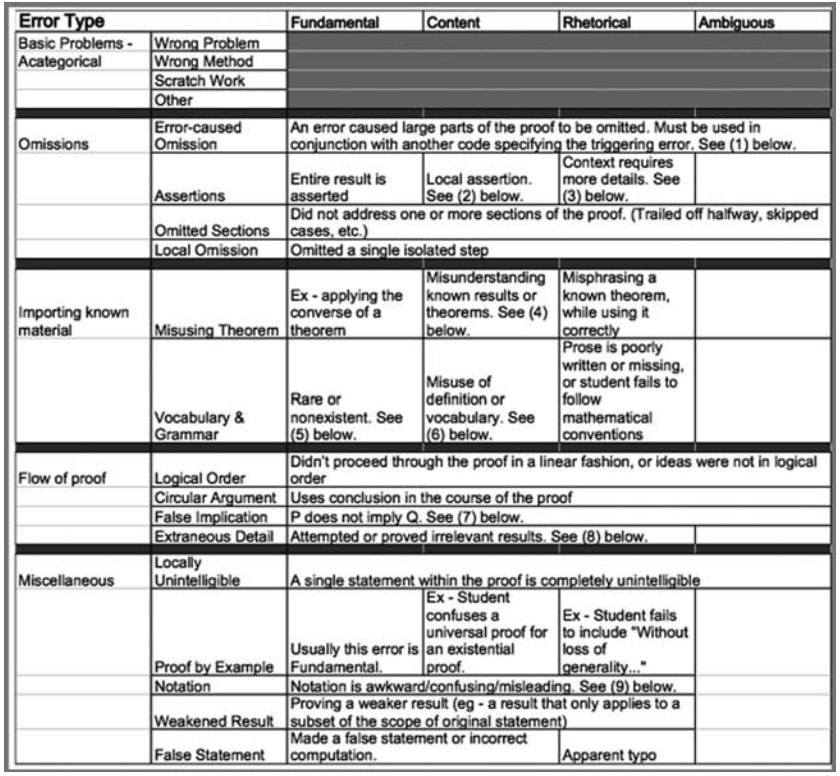
\includegraphics[width=\linewidth]{Error/Strickland&Rand_CodingSchemeMatrix(Fig1_PRIMUS_26_10_905-921)}
\end{figure}

The rows of the coding scheme represent the type of error and the columns represent the severity of the error. Please refer to the Appendix of \cite[Figure 1]{Strickland_2016} for a more detailed description of these error classifications.

\subsection{Abbreviated Error Codes}
To streamline the use of the error classification we will use the following system for abbreviating the error classifications:

%Error types will be read from Figure \ref{fig-sr-err} as ``Column Row", i.e., ``Severity Type". For instance, we may encounter a ``Content Misusing Theorem'' error or a ``Fundamental Logical Order'' error. This convention informs the following system of abbreviations:

\begin{figure}[h]
\caption{`Severity of error' codes}\label{fig-code-severe}
\begin{multicols}{2}
\begin{description}
\item[F] Fundamental	
\item[C] Content
\item[N] Novice \footnotemark
\item[A] Ambiguous
\end{description}
\end{multicols}
\end{figure}

\footnotetext{In this document, we use ``Novice'' in place of Strickland and Rand's descriptor ``Rhetorical". }

%\vspace{-0.75cm}

\begin{figure}[h]
\caption{`Type of error' codes}\label{fig-code-type}
\begin{multicols}{2}
\begin{description}
\item[WP] Wrong Problem
\item[WM] Wrong Method
\item[SW] Scratch Work
\item[EO] Error-caused Omission \footnotemark
\item[A] Assertions
\item[OS] Omitted Sections
\item[O] Omission / Local Omission
\item[MT] Misusing Theorem
\item[VG] Vocabulary \& Grammar
\item[Log] Logical Order
\item[Cir] Circular Argument
\item[FI] False Implication
\item[ED] Extraneous Detail
\item[LU] Locally Unintelligible
\item[Eg] Proof by Example
\item[N] Notation
\item[WR] Weakened Result
\item[FS] False Statement
%\item[Misc] Miscellaneous / Other
\end{description}
\end{multicols}
\end{figure}

\footnotetext{Note that the Error-caused Omission code must always be used in conjunction with a second error type (and severity) code for the original error that caused the subsequent omission. We will use a hyphen/parentheses to indicate such an error. For example, if an omission occurred as a result of misunderstanding a known theorem. this would be an Error-caused Omission resulting from a Content Misusing Theorem error, and it would be abbreviated as EO-(C-MT).}

For example, using these abbreviations, a Content Misusing Theorem error will be abbreviated by C-MT and a Fundamental Logical Order error will be abbreviated by F-Log. Using Strickland and Rand's scheme, the errors Wrong Problem, Wrong Method, and Scratch Work do not have severity ratings.



%%%%% I removed the below now about MISC because it looks like we don't use MISC anywhere in this document. I also commented it out above.

%Moreover, our use of `Miscellaneous' is different from Strickland and Rand's but agrees with their use of `Other' \cite{Strickland_2016}.





%----------------------PART TWO RESOURCES-----------------------------
\part{Flawed Proofs}\label{part-proofs}

%----------------------CHAPTER THREE STATEMENTS, LOGIC, ELEMENTARY NUMBER THEORY
\chapter{Elementary Topics}\label{ch-element}
The topics covered in this chapter fit into the first halves of MATH 271 Discrete Mathematics and MATH 273 Numbers and Proofs at the University of Calgary, but are also common to many courses serving as an introduction to mathematical proof.  Topics include
\begin{itemize}
 	\item divisibility, the gcd and modular arithmetic
 	\item definition of even and odd integers, and
 	\item basic properties of rational and real numbers.
\end{itemize}
In these exercises and proofs, learners are confronted with familiar notions from school mathematics in the unfamiliar setting of mathematical rigour.

Given its importance as proof technique, and its difficulty for the novice learner,
Mathematical Induction, is covered in its own dedicated chapter (see Chapter \ref{ch-ind}).

%-----------------%-----------------%%
% Author: Christian Bagshaw
% Date: August 2020
% Revised: JMS; 22 January 2021
% Lauren DeDieu, Jerrod M.~Smith, Kimberly Golubeva and Christian Bagshaw
% A Resource Bank for Writing Intensive Mathematics Courses
% This work is licensed under a  Creative Commons Attribution-NonCommercial-ShareAlike 4.0 International License
% http://creativecommons.org/licenses/by-nc-sa/4.0/
\section{Logic}

\begin{xca}[Converse of a Statement]{xca:converse-1}
Let $n$ be an integer. Prove or disprove the converse and contrapositive of the following statement:\\

If $n$ is a positive integer, then $n + 3$ is a positive integer. 
\end{xca}

\begin{flaw}{flaw:converse-1}
The converse of the statement is ``if $n+3$ is a positive integer, then $n$ is a positive integer". This statement is true. If $n+3$ is positive we can say $n+3 > 0$, which means $n > 0$, so $n$ is positive. \\

The contrapositive of the statement is ``if $n+3$ is not a positive integer, then $n$ is a positive integer". This statement is false. We will provide a counterexample to show this. If $n = -4$, then $n+3 = -1$ is not a positive integer, but $n = -4$ is also not a positive integer. 
\end{flaw}

\clearpage
\subsection{Error classification}


There are several errors
 in the Flawed Proof \ref{flaw:converse-1}.

 \begin{description}
    \item[F-FI] The implication that $n+3 > 0$ means $n > 0$ is false. 
    \item[WP] ``If $n+3$ is not a positive integer, then $n$ is a positive integer" is not the contrapositive of the statement 
 	
 \end{description}

\subsubsection{Error codes}
\begin{itemize}
	\item 	Fundamental False Implication (F-FI)
	\item Wrong Problem (WP)
\end{itemize}
See Section \ref{sec-error} for more information about error classifications.

\clearpage
\subsection{Corrected proof}

The following is a corrected version of Flawed Proof \ref{flaw:converse-1}. 

\begin{prf}{prf:proof1} 
Let $n\in \Z$.

The converse of the statement is ``if $n+3$ is a positive integer, then $n$ is a positive integer". This statement is false. We will provide a counterexample. Let $n = -1$. We have that $n+3 = 2$ is positive, but $n = -1$ is negative.\\

The contrapositive of the statement is ``if $n+3$ is not a positive integer, then $n$ is not a positive integer". This statement is true. Here is a proof:

Suppose that $n+3$ is not a positive integer. Then $n+3 \leq 0$. This means $n+3 - 3 \leq 0 - 3$, so $n \leq -3 \leq  0$. Therefore $n$ is not a positive integer. 
\end{prf} %MATH 271; revised
% Author: Christian Bagshaw
% Date: August 2020
% Revised: JMS; 22 January 2021
% Lauren DeDieu, Jerrod M.~Smith, Kimberly Golubeva and Christian Bagshaw
% A Resource Bank for Writing Intensive Mathematics Courses
% This work is licensed under a  Creative Commons Attribution-NonCommercial-ShareAlike 4.0 International License
% http://creativecommons.org/licenses/by-nc-sa/4.0/
\section{Divisibility of a Product}

\begin{xca}[Divisibility of a Product]{xca:div-prod}
Let $a,b$ and $c$ be integers. Prove that if $a$ divides $b$, then $a$ divides $bc$. 
\end{xca}

\begin{flaw}{flaw:div-prod} 
Suppose $a$ is even. Since $a$ divides $b$ this means $b$ is even. Therefore $bc$ is even, so that means $a$ divides $bc$. 
\end{flaw}

\clearpage
\subsection{Error classification}

There are multiple errors
 in the Flawed Proof \ref{flaw:div-prod}. 

 
 \begin{description}
    \item[WM]  There is no need to suppose the case that $a$ is even.
    \item[EO-(WM)] The flawed proof has not considered the case where $a$ is odd. 
    \item[N-A] The assertion ``since $a$ divides $b$ this means $b$ is even" requires more details. 
    \item[F-FI] The implication  ``$bc$ is even, so that means $a$ divides $bc$" is false. 
 	
 \end{description}

 
\subsubsection{Error codes}
\begin{itemize}
    \item Wrong Method (WM)
    \item Error Caused Ommision Wrong Method (EO-(WM))
    \item Novice Assertion (N-A)
	\item 	Fundamental False Implication (F-FI). 
\end{itemize}
See Section \ref{sec-error} for more information about error classifications.

\clearpage
\subsection{Corrected proof}

The following is a corrected version of Flawed Proof \ref{flaw:div-prod}. 

\begin{prf}{prf:div-prod} 
Suppose that $a,b \in \Z$ and suppose that $a$ divides $b$.
Since $a$ divides $b$, there exists some integer $k$ such that $ak = b$. Multiplying both sides by $c$ gives us that $akc = bc$. We will let $kc = l$, and note that $l$ is an integer. Thus $al = bc$, so by definition $a$ divides $bc$. 

\end{prf} %MATH 271; revised
%Author: Kimberly Golubeva
%Date: July 14, 2020
% Revised: JMS; 22 January 2021
% Lauren DeDieu, Jerrod M.~Smith, Kimberly Golubeva and Christian Bagshaw
% A Resource Bank for Writing Intensive Mathematics Courses
% This work is licensed under a  Creative Commons Attribution-NonCommercial-ShareAlike 4.0 International License
% http://creativecommons.org/licenses/by-nc-sa/4.0/
\section{Contrapositive and Converse}

\begin{xca}[]{xca:contraconv}
Let $n$ be an integer.
Write the contrapositive and the converse of the true statement \\
$$``\text{If } n > 2, \text{ then } n^2 > 4."$$
Is the contrapositive true? Is the converse true? Explain why or why not. 
\end{xca}

\begin{flaw}{flaw:contraconv}
\begin{enumerate}
\item Contrapositive: If $n^2 < 4$, then $n < 2.$ 
\item Converse: If $n^2>4$, then $n>2$. \\
\end{enumerate}
As the original statement is true, and the contrapositive is logically equivalent to the original statement, the contrapositive is true. Despite the fact that the converse is not logically equivalent to the original statement, in this case, the converse is true. Taking the square root of both sides of $n^2>4$
$$\sqrt{n^2} > \sqrt{4},$$
we see that this statement implies that $n > 2.$
\end{flaw}

\clearpage
\subsection{Error classification}



There are several errors
% is only one error ... etc.
 in the Flawed Proof \ref{flaw:contraconv}. 

 
\subsubsection{Error codes}

\begin{description}
 	\item[C-O:] Failed to recognize that 'not greater than' is equivalent to 'less than or equal to', which lead to the omission of the 'or equal to' from the statement of the contrapositive.
 	\item[C-FS-EO:] The statement that $\sqrt{n^2} > \sqrt{4}$ implies $n > 2$ is false. This error caused the omission of the case where $n$ is negative, which is the key element of the proof. 
 \end{description}

 
\subsubsection{Error codes}
\begin{itemize}
	\item 	Content Local Omission (C-O)
	\item   Content False Statement Error Caused Omission (C-FS-EO)
\end{itemize}
See Section \ref{sec-error} for more information about error classifications.

\clearpage
\subsection{Corrected proof}

The following is a corrected version of Flawed Proof \ref{flaw:contraconv}. 

\begin{prf}{prf:contraconv} 
Let $n$ be an integer.
\begin{enumerate}
\item Contrapositive: If $n^2 \leq 4$, then $n \leq 2.$ 
\item Converse: If $n^2>4$, then $n>2$. \\
\end{enumerate}
As the original statement is true, and the contrapositive is logically equivalent to the original statement, the contrapositive is true. 

However, the converse is not logically equivalent to the original statement and in this case, the converse is false. 

Indeed, the negation of the converse is: ``$n^2 > 4$ but $n \leq 2$." Here is a proof:
Consider $n = -5$. Then $n^2 = 25$, which is greater than $4$, but $-5$ is not greater than $2.$
\end{prf} %MATH 271; revised
% Author: Kimberly Golubeva
% Date: 13 July 2020
% Revised: JMS; 22 January 2021
% Lauren DeDieu, Jerrod M.~Smith, Kimberly Golubeva and Christian Bagshaw
% A Resource Bank for Writing Intensive Mathematics Courses
% This work is licensed under a  Creative Commons Attribution-NonCommercial-ShareAlike 4.0 International License
% http://creativecommons.org/licenses/by-nc-sa/4.0/
\section{Properties of Integers}

\begin{xca}{xca:negevenint}
Prove that the negative of any even integer is even. 
\end{xca}

\begin{flaw}{flaw:negevenint}
Suppose that $n$ is any even integer. By the definition of even, $n=2k$ for some integer $k$. The negative of $n$ is equal to $-n$. Thus, $-n = -2k.$ By dividing both sides of the equation by $-1$, we get back the original equation of $n=2k$. Therefore, the negative of any integer $n$ is an even number. 
\end{flaw}

\clearpage
\subsection{Error classification}


There are several errors
% is only one error ... etc.
 in the Flawed Proof \ref{flaw:negevenint}. 
 
\begin{description}
 	\item[N-N:] Awkward phrasing. Instead, write how the equation $-n=-2k$ was obtained.	
 	\item[C-FI:] The equation $n=2k$ does not inherently imply that $-n$ is even.
 	\item [F-A:] The entire result is asserted by stating that $n=2k$ implies that $-n$ is even.
 \end{description}

 
\subsubsection{Error codes}
\begin{itemize}
	\item 	Novice Notation (N-N)
	\item   Content False Implication (C-FI)
	\item   Fundamental Assertion (F-A)
\end{itemize}
See Section \ref{sec-error} for more information about error classifications.

\clearpage
\subsection{Corrected proof}

The following is a corrected version of Flawed Proof \ref{flaw:negevenint}. 

\begin{prf}{prf:negevenint} 
Suppose that $n$ is an even integer. Then $n=2k$ for some integer $k$. Multiplying both sides by $-1 \in \mathbb{Z}$, we obtain the equation $-n=-2k$. Moreover, we have
\[-n = -2k = 2(-k),\]
where $-k$ is an integer.  Thus, $-n$ is also even. 
\end{prf}
 %MATH 271; revised
% Author: Kimberly Golubeva
% Date: 13 July 2020
% Revised: JMS; 22 January 2021
% Lauren DeDieu, Jerrod M.~Smith, Kimberly Golubeva and Christian Bagshaw
% A Resource Bank for Writing Intensive Mathematics Courses
% This work is licensed under a  Creative Commons Attribution-NonCommercial-ShareAlike 4.0 International License
% http://creativecommons.org/licenses/by-nc-sa/4.0/
\section{The Rationals}

\begin{xca}{xca:intaddfrac}
Prove or disprove the following statement. For all integers $m$ and $n$, if $m, n > 1$, then $\frac1m + \frac1n$ is not an integer.
\end{xca}

\begin{flaw}{flaw:intaddfrac}
Suppose that $m$ and $n$ are integers and that $m,n > 1$. Since $\frac1m$ is the reciprocal of $m$ and it is not an integer and $\frac1n$ is the reciprocal of $n$ and it is not an integer, then there are no two distinct numbers such that $\frac1m + \frac1n$ can ever be an integer.
\end{flaw}

\clearpage
\subsection{Error classification}


There are several errors
% is only one error ... etc.
 in the Flawed Proof \ref{flaw:intaddfrac}. 

\subsubsection{Error codes}

\begin{description}
 	%\item[F-FS:] The statement that $\frac1{m}$ implies that $\frac1m$ + $\frac1n$ cannot be an integer is false.
 	\item[C-FI:] The statement that $\frac1{m}$ and $\frac1{n}$ are not integers implies that $\frac1m + \frac1n$ is not an integer is false.
 	%\item[C-OS:] Did not consider the case where $m=n$.
 	\item[F-A:] Asserted the entire result.
 \end{description}


\subsubsection{Error codes}
\begin{itemize}
	%\item 	Fundamental False Statement (F-FS)
	\item   Content False Implication (C-FI)
	%\item   Content Omitted Sections (C-OS)
	\item   Fundamental Assertion (F-A)
\end{itemize}
See Section \ref{sec-error} for more information about error classifications.

\clearpage
\subsection{Corrected proof}

The following is a corrected version of Flawed Proof \ref{flaw:intaddfrac}. 

\begin{prf}{prf:intaddfrac} 
This statement is false. Its negation is: there exist integers $m$ and $n$ so that $m>1$, $n>1$ and $\frac1m + \frac1n$ is an integer. Here's a proof:

Let $m,n = 2$. Then $m,n > 1$ and $\frac1m+ \frac1n = \frac12 + \frac12 = 1 \in \mathbb{Z}.$
\end{prf}  %MATH 271; revised
% Author: Kimberly Golubeva
% Date: unknown
% Revised: JMS 3 Feb 2021
% Lauren DeDieu, Jerrod M.~Smith, Kimberly Golubeva and Christian Bagshaw
% A Resource Bank for Writing Intensive Mathematics Courses
% This work is licensed under a  Creative Commons Attribution-NonCommercial-ShareAlike 4.0 International License
% http://creativecommons.org/licenses/by-nc-sa/4.0/
\section{Divisibility}

\begin{xca}{xca:divisibility_sum}
Prove that for any integers $a,b$ and $c$, if $a \mid b$ and $a \mid c$ then $a \mid (b+c).$
\end{xca}

\begin{flaw}{flaw:divisibility_sum} 
We will consider two cases. 
First, let $a$ be odd. Then we can randomly choose the values $a = 5$, $b = 30$ and $c=10$ to show that $a \mid (b+c)$. We know that $$\frac{30}{5} = 6 \quad\text{and} \quad \frac{10}{5} = 2.$$
Additionally, we have that $b+c = 30 + 10 = 40$. This implies
$$\frac{40}{5} = 8,$$
which means that $a \mid (b+c)$ when $a$ is odd. 

Now, let $a$ be even. Then we can randomly choose the values $a = 2$, $b = 12$ and $c=10$ to show that $a \mid (b+c)$. We know that $$\frac{12}{2} = 6 \quad\text{and} \quad \frac{10}{2} = 5.$$
Additionally, we have that $b+c = 12 + 10 = 22$. This implies
$$\frac{22}{2} = 11,$$
which means that $a \mid (b+c)$ when $a$ is even.
\end{flaw}

\clearpage
\subsection{Error classification}



There are several errors
% is only one error ... etc.
 in the Flawed Proof \ref{flaw:divisibility_sum}. 

 
 \begin{description}
 	\item[EO-F-Eg:] Here, proof by example leads to the omission of nearly all cases, except the ones given in the example. Additionally, there is a fundamental error in the failure to recognize that 'randomly' choosing a specific example is not sufficient evidence to prove a statement with a universal quantifier.
 	\item[F-WM:] Dividing the proof into two cases is not the correct approach. Moreover, the definition of `divides' is not explicitly used in the proof. 
 \end{description}

 
\subsubsection{Error codes}
\begin{itemize}
	\item 	Fundamental Error-caused Omission -- Fundamental -- due to Proof by Example (EO-F-Eg)
	\item Fundamental Wrong Method (F-WM)
\end{itemize}
See Section \ref{sec-error} for more information about error classifications.

\clearpage
\subsection{Corrected proof}

The following is a corrected version of Flawed Proof \ref{flaw:divisibility_sum}. 

\begin{prf}{prf:divisibility_sum} 
Suppose that $a, b$ and $c$ are integers and that $a \mid b$ and $a \mid c$. By the definition of divisibility, we have that $b = ja$ and $c = ka$ for some integers $j$ and $k$. Then
$$b + c = ja + ka = a(j+k),$$
where $j+k$ is also an integer, since it is the sum of two integers. Thus, by the definition of divisibility, it follows that  $a \mid (b+c)$.
\end{prf}
 %MATH 271; revised
% Author: Christian Bagshaw
% Date: DD MMM 2020
% Lauren DeDieu, Jerrod M.~Smith, Kimberly Golubeva and Christian Bagshaw
% A Resource Bank for Writing Intensive Mathematics Courses
% This work is licensed under a  Creative Commons Attribution-NonCommercial-ShareAlike 4.0 International License
% http://creativecommons.org/licenses/by-nc-sa/4.0/
\section{Divisibility and Modular Arithmetic}

\begin{xca}[Basic Divisibility Property]{xca:divmodarith}
Let $a,b$ be integers. Prove that $b \equiv 0 \mod a$ if and only if $a$ divides $b$. 
\end{xca}

\begin{flaw}{flaw:divmodarith} %change the label
If $b \equiv 0 \mod a$, then $0$ divides $b-a$. So there exists some integer $n$ such that $b+0 = na$. So $a$ divides $b$. 
\end{flaw}

\clearpage
\subsection{Error classification}

%Provide a brief classification and explanation of the errors in the Flawed Proof \ref{flaw:proof1}. %change the label

There are multiple errors
 in the Flawed Proof \ref{flaw:divmodarith}. 
 
 \begin{description}
  \item[C-VG] Incorrect understanding of what $b \equiv 0 \mod a$ means. 
  \item[C-VG] Incorrect understanding of divisibility.
    \item[F-OS]  Did not address one direction of the ``if and only if" proof. 
 	
 \end{description}

 
\subsubsection{Error codes}
\begin{itemize}
    \item Content Vocabulary and Grammar (C-VG)
    \item Fundamental Omitted Sections (F-OS)
\end{itemize}
See Section \ref{sec-error} for more information about error classifications.

\clearpage
\subsection{Corrected proof}

The following is a corrected version of Flawed Proof \ref{flaw:divmodarith}. %change the label

\begin{prf}{prf:divmodarith} %change the label
Let $a,b$ be integers. Firstly suppose $b \equiv 0 \mod a$. By definition, this means $a$ divides $b-0$. But since $b-0 = 0$, we conclude $a$ divides $b$. 

Conversely suppose $a$ divides $b$. Then since $b = b-0$, we can say $a$ divides $b-0$. Thus by definition, $b \equiv 0 \mod a$.  
\end{prf} %MATH 271;
% Author: Kimberly Golubeva
% Date: 27 July 2020
% Revised: JMS 3 Feb 2020
% Lauren DeDieu, Jerrod M.~Smith, Kimberly Golubeva and Christian Bagshaw
% A Resource Bank for Writing Intensive Mathematics Courses
% This work is licensed under a  Creative Commons Attribution-NonCommercial-ShareAlike 4.0 International License
% http://creativecommons.org/licenses/by-nc-sa/4.0/
\section{Proof by Contrapositive}

\begin{xca}{xca:contra_parity}
Let $x \in \mathbb{Z}.$ Prove that if $x^2-6x+5$ is even, then $x$ is odd.  
\end{xca}

\begin{flaw}{flaw:contra_parity} 
Suppose that $x^2-6x+5$ is even. We want to prove that $x$ is odd. By the definition of even, $x^2-6x+5 = 2k$ for some integer $k.$ So we have $x^2-6x+5 = 2k$ and, rearranging, $x^2-6x+(5-2k) = 0$. Then, using the quadratic formula, 
\begin{align*}
    x &= \frac{6 \pm \sqrt{6^2 - 4(1)(5-2k)}}{2} \\
    &= \frac{6 \pm \sqrt{36 - 20 + 8k}}{2} \\
    &= \frac{6 \pm\sqrt{16 + 8k}}{2}\;.
\end{align*}
Now we must show that $x = \frac{6 \pm\sqrt{16 + 8k}}{2}$ is odd. That is, we must show that $\frac{6 \pm\sqrt{16 + 8k}}{2} = 2j+1$ for some integer $j.$ So
\begin{align*}
    \frac{6 \pm\sqrt{16 + 8k}}{2} &= \frac{1}{2}\left(6 \pm \sqrt{16+8k}\right) \\
    &= \frac{1}{2}\left(6 \pm \sqrt{16}\sqrt{8k}\right) \\ 
    &= \frac{1}{2}\left(6 \pm 4\sqrt{8k}\right) 
\end{align*}
... not enough time to finish.
\end{flaw}

\clearpage
\subsection{Error classification}

There are several errors
% is only one error ... etc.
 in the Flawed Proof \ref{flaw:contra_parity}. 

 
 \begin{description}
 	\item[F-WM:] A direct proof may not be available with elementary methods.  An indirect proof (by contradiction, or proving the contrapositive) will be more effective .
 	\item[F-FS:] $\frac{1}{2}\left(6 \pm \sqrt{16+8k}\right) \neq \frac{1}{2}\left(6 \pm \sqrt{16}\sqrt{8k}\right).$
 	
 \end{description}

 
\subsubsection{Error codes}
\begin{itemize}
	\item 	Fundamental Wrong Method (F-WM)
	\item Fundamental False Statement (F-FS)
\end{itemize}
See Section \ref{sec-error} for more information about error classifications.

\clearpage
\subsection{Corrected proof}

The following is a corrected version of Flawed Proof \ref{flaw:contra_parity}. 

\begin{prf}{prf:contra_parity} 
We will prove the contrapositive of this statement. That is, we prove that if $x$ is even, then $x^2-6x+5$ is odd. To do so, suppose that $x$ is even and write $x = 2k$ for some integer $k.$ Then
\begin{align*}
    x^2-6x+5 &= (2k)^2 - 6(2k) + 5 \\
    &= 4k^2 - 12k + 5 \\
    &= 2(2k^2-6k+2)+1.
\end{align*}
Now, since $2k^2-6k+2 \in \Z$, it follows that $x^2-6x+5$ is odd. Thus, since the contrapositive is true and it is logically equivalent to  the original statement, we can conclude that the original statement is true.
\end{prf} %MATH 271; revised
% Author: Kimberly Golubeva
% Date: 21 July 2020
% Revised: 
% Lauren DeDieu, Jerrod M.~Smith, Kimberly Golubeva and Christian Bagshaw
% A Resource Bank for Writing Intensive Mathematics Courses
% This work is licensed under a  Creative Commons Attribution-NonCommercial-ShareAlike 4.0 International License
% http://creativecommons.org/licenses/by-nc-sa/4.0/
\section{Modular Arithmetic and Divisibility}

\begin{xca}{xca:direct_mod}
Let $p$ be an integer and suppose that $p$ is not divisible by $3.$ Prove that $p^2 \equiv 1 \text{ (mod } 3).$
\end{xca}

\begin{flaw}{flaw:direct_mod} 
Since $3 \nmid p$, this implies that we have two cases. Namely, either \\
$p \equiv 1 \text{ (mod } 3)$ or $p \equiv 2 \text{ (mod } 3)$. \\ 

\noindent \textbf{Case 1:} $p \equiv 1 \text{ (mod } 3)$. By definition, $p = 3k+1$ for some integer $k.$ Then
\begin{align*}
    p^2 &= (3k+1)^2 \\
    &= 9k^2 + 6k +1 \\
    & = 3\left(3k^2+2k + \frac{1}{3}\right)
\end{align*}
I'm not sure where to go from here...\\

\noindent \textbf{Case 2:} $p \equiv 2 \text{ (mod } 3)$. By definition, $p = 3k+2$ for some integer $k.$ Then
\begin{align*}
    p^2 &= (3k+2)^2 \\
    &= 9k^2 + 12k +4 \\
    & = 3\left(3k^2+4k+\frac43\right)
\end{align*}
I'm not sure where to go from here...
\end{flaw}

\clearpage
\subsection{Error classification}


There is only one error
 in the Flawed Proof \ref{flaw:direct_mod}.

 
 \begin{description}
 	\item[C-OS:] Failed to recognize that the first few terms in the expressions $9k^2 + 6k +1$ and $9k^2 + 12k +4$ can be factored independently of the last term, leading to the omission of the final steps in both cases. 
 \end{description}

 
\subsubsection{Error codes}
\begin{itemize}
	\item 	Content Omitted Sections (C-OS)
\end{itemize}
See Section \ref{sec-error} for more information about error classifications.

\clearpage
\subsection{Corrected proof}

The following is a corrected version of Flawed Proof \ref{flaw:direct_mod}.

\begin{prf}{prf:direct_mod}
Since $3 \nmid p$, this implies that we have two cases. Namely, either \\
$p \equiv 1 \text{ (mod } 3)$ or $p \equiv 2 \text{ (mod } 3)$. \\ 

\noindent \textbf{Case 1:} $p \equiv 1 \text{ (mod } 3)$. By definition, $p = 3k+1$ for some integer $k.$ Then
\begin{align*}
    p^2 &= (3k+1)^2 \\
    &= 9k^2 + 6k +1 \\
    & = 3(3k^2+2k)+1 \\
    & = 3l + 1
\end{align*}
where $l \eqdef 3k^2+2k$ is an integer. Thus, $p^2 \equiv 1 \text{ (mod } 3).$ \\

\noindent \textbf{Case 2:} $p \equiv 2 \text{ (mod } 3)$. By definition, $p = 3k+2$ for some integer $k.$ Then
\begin{align*}
    p^2 &= (3k+2)^2 \\
    &= 9k^2 + 12k +4 \\
    &= 9k^2 + 12k +3 + 1 \\
    & = 3(3k^2+4k+1)+1 \\
    & = 3l + 1
\end{align*}
where $l \eqdef 3k^2+4k+1$ is an integer. Thus, $p^2 \equiv 1 \text{ (mod } 3).$

\end{prf}
 %MATH 273
% Author: Christian Bagshaw
% Date: August 2020
% Revised: JMS 23 September 2020
% Lauren DeDieu, Jerrod M.~Smith, Kimberly Golubeva and Christian Bagshaw
% A Resource Bank for Writing Intensive Mathematics Courses
% This work is licensed under a  Creative Commons Attribution-NonCommercial-ShareAlike 4.0 International License
% http://creativecommons.org/licenses/by-nc-sa/4.0/
\section{GCD}

\begin{xca}[Multiple of $\gcd$]{xca:gcd_multiple}
Let $a$ and $b$ be positive integers. For any positive integer $n$ prove $\gcd(na, nb) = n\gcd(a,b)$. 
\end{xca}

\begin{flaw}{flaw:gcd_multiple} 
Let $\gcd(a,b) = d$. Then we can write $a = dk$ and $b = dl$ for some integers $k,l$. Let $\gcd(na, nb) = \gcd(ndk, ndl) = n\gcd(dk, dl) = n\gcd(a,b)$. 

\end{flaw}

\clearpage
\subsection{Error classification}



There are several errors
% is only one error ... etc.
 in the Flawed Proof \ref{flaw:gcd_multiple}. 
 
 \begin{description}
    \item[N-VG] Incorrect use of the word ``let" in the final statement. Something is being asserted, so  ``therefore" or ``thus" should be used. 
    \item[F-A ] The entire result is asserted in the final statement without proof. 
 	
 \end{description}

 
\subsubsection{Error codes}
\begin{itemize}
	\item Novice Vocabulary Grammar (N-VG)
	\item Fundamental Assertion (F-A)
\end{itemize}
See Section \ref{sec-error} for more information about error classifications.

\clearpage
\subsection{Corrected proof}

The following is a corrected version of Flawed Proof \ref{flaw:gcd_multiple}. %change the label

 % Corrected proof revised 23 September 2020 by Jerrod
\begin{prf}{prf:gcd_multiple} %change the label
Let $d = \gcd(a,b)$ and $c = \gcd(na, nb)$. We wish to show $nd = c$. By the definition of the greatest common divisor, we know $d\, |\, a$ and $d\, | \,b$.  In particular, $a = dk$ and $b=d\ell$ for some (positive) integers $k,\ell \in \Z$.  Moreover, $na = ndk$ and $nb = nd\ell$, so it follows that  $nd \, | \,na$ and $nd \, | \, nb$. 
%By the definition of the greatest common divisor, we must have $nd \leq c$.
Since $c = \gcd(na, nb)$, there exist integers $x$ and $y$ so that $c = xna + ynb$.
Substituting $na = ndk$ and $nb = nd\ell$ we obtain \[ c = xndk + ynd\ell = nd(xk + y\ell),\]
where $xk + y\ell \in \Z$, thus $nd$ divides $c$.
So we can write $c = ndt$ for some positive integer $t \in \mathbb{Z}$. 
Since $c=\gcd(na,nb)$ divides both $na$ and $nb$, 
we can now say $ndt \, | \, na$ and $ndt \, | \, nb$.
That is, there are integers $p$ and $q$ so that $na = ndtp$ and $nb = ndtq$.  Dividing by $n$, we obtain $a = dtp$ and $b=dtq$, which implies $dt \, | \, a$ and $dt \, | \, b$. 
But by the definition of $\gcd(a,b)$ this means $dt \leq d$, which means $t = 1$ (because $d$ and $t$ are positive). Therefore $nd = c$.
\end{prf} % MATH 271/273; revised
%Author: Kimberly Golubeva
%Date: July 14 2020
% Lauren DeDieu, Jerrod M.~Smith, Kimberly Golubeva and Christian Bagshaw
% A Resource Bank for Writing Intensive Mathematics Courses
% This work is licensed under a  Creative Commons Attribution-NonCommercial-ShareAlike 4.0 International License
% http://creativecommons.org/licenses/by-nc-sa/4.0/
\clearpage
\section{The Parity Property}

\begin{xca}[]{xca:parityproperty}
Prove that any two consecutive integers have opposite parity. 
\end{xca}

\begin{flaw}{flaw:parityproperty}
Let $n \in \mathbb{Z}$ and suppose that $n$ is even. By definition. $n=2k$ and so $n+1 = 2k+1$, which is odd. Thus, any two consecutive integers have opposite parity. 
\end{flaw}

\clearpage
\subsection{Error classification}

%Provide a brief classification and explanation of the errors in the Flawed Proof \ref{flaw:proof1}. %change the label

There are several errors
% is only one error ... etc.
 in the Flawed Proof \ref{flaw:parityproperty}. 
 
\subsubsection{Error codes}

\begin{description}
 	\item[C-OS:] The case where $n$ is odd was assumed to be true and therefore omitted from the proof.  
 	\item[C-N:] Failed to define what the variable $k$ is. 
 \end{description}

\subsubsection{Error codes}
\begin{itemize}
	\item 	Content Omitted Sections (F-FS)
	\item   Content Notation (C-N)
\end{itemize}
See Section \ref{sec-error} for more information about error classifications.

\clearpage
\subsection{Corrected proof}

The following is a corrected version of Flawed Proof \ref{flaw:parityproperty}. %change the label

\begin{prf}{prf:parityproperty} %change the label
Let $n \in \mathbb{Z}$. We have two cases: 

\begin{enumerate}
    \item \textbf{$n$ is even:} By definition, $n = 2k$ for some integer $k$. Then $n+1 = 2k+1$, which is odd.
    \item \textbf{$n$ is odd:} By definition, $n=2k+1$ for some integer $k$. Then $$n+1 = (2k+1) +1 = 2k+2 = 2(k+1),$$
    which is even since it equals twice some integer $k+1$.
\end{enumerate}
Thus, any two consecutive integers have opposite parity.  
\end{prf} %MATH 273
% Author: Christian Bagshaw
% Date: August 2020
% Lauren DeDieu, Jerrod M.~Smith, Kimberly Golubeva and Christian Bagshaw
% A Resource Bank for Writing Intensive Mathematics Courses
% This work is licensed under a  Creative Commons Attribution-NonCommercial-ShareAlike 4.0 International License
% http://creativecommons.org/licenses/by-nc-sa/4.0/
\section{Infinitude of Primes}

\begin{xca}[Infinitude of Primes]{xca:inf-prime}
Prove there exist infinitely many prime numbers.  
\end{xca}

\begin{flaw}{flaw:inf-prime} %change the label
Let $p_1, ..., p_k$ be the set of all prime numbers, where $k$ is some positive integer. Now let $N = p_1...p_k + 1$. Now we see that $N$ is not divisible by any of $p_1, ..., p_k$. But we know all integers greater than 1 can be written as a product of primes. Therefore $N$ is prime. This contradicts letting $p_1, ..., p_k$ being the set of all prime numbers. 
\end{flaw}

\clearpage
\subsection{Error classification}

%Provide a brief classification and explanation of the errors in the Flawed Proof \ref{flaw:proof1}. %change the label

There are multiple errors
 in the Flawed Proof \ref{flaw:inf-prime}. %change the label

 
 \begin{description}
    \item[N-VG]  The flawed proof uses proof by contradiction. To set this up, the proof states ``let $p_1, ..., p_k$ be the set of all prime numbers", intending to derive a contradiction. Mathematical convention is to use the word ``assume", because we are assuming a false claim that will be contradicted.  
    \item[C-FI]  The implication that ``N is not divisible by any of $p_1, ..., p_k$ ... Therefore N is prime" is false.  
 	
 \end{description}

 
\subsubsection{Error codes}
\begin{itemize}
    \item Novice Vocabulary Grammar (N-VG)
	\item 	Content False Implication (C-FI). 
\end{itemize}
See Section \ref{sec-error} for more information about error classifications.

\clearpage
\subsection{Corrected proof}

The following is a corrected version of Flawed Proof \ref{flaw:inf-prime}. %change the label

\begin{prf}{prf:inf-prime} %change the label
Assume there are finitely many primes, we will derive a contradiction. Let $p_1, ..., p_k$ be the set of all prime numbers, where $k$ is some positive integer. Now let $N = p_1...p_k + 1$. Now we see that $N$ is not divisible by any of $p_1, ..., p_k$. But we know all integers greater than 1 can be written as a product of primes. Therefore $N$ has a prime factor that is not one of $p_1, ..., p_k$. So our list of all primes is not complete - a contradiction. Therefore there must be infinitely many primes. 
\end{prf} %MATH 273
%April 20 2021 % Author: Kimberly Golubeva
% Date: 20 April 2020
% Lauren DeDieu, Jerrod M.~Smith, Kimberly Golubeva and Christian Bagshaw
% A Resource Bank for Writing Intensive Mathematics Courses
% This work is licensed under a  Creative Commons Attribution-NonCommercial-ShareAlike 4.0 International License
% http://creativecommons.org/licenses/by-nc-sa/4.0/
\section{Divisibility of a Product }

\begin{xca}{xca:divis_product_wrongdef}
Let $a,b$ and $c$ be integers. Prove that if $a$ divides $b$, then $a$ divides $bc$. 
\end{xca}

\begin{flaw}{flaw:divis_product_wrongdef} %change the label
Suppose $a \mid b$. Then $a = bk$ for some $k \in \mathbb{Z}.$ Then if we multiply by $c$ on both sides, we get
\[ ac = bck\;. \]
Since $c$ is any integer, let $c=1$. Then
\[ a = bck\;, \]
which means that $a$ divides $bc$ since $a = (bc)k$, where $k$ is an integer. 

\end{flaw}

\clearpage
\subsection{Error classification}

%Provide a brief classification and explanation of the errors in the Flawed Proof \ref{flaw:proof1}. %change the label

There are several errors
% is only one error ... etc.
 in the Flawed Proof \ref{flaw:divis_product_wrongdef}. %change the label

 
 \begin{description}
 	\item[C- VG: ] The statement that $a$ divides $b$ implies $a = bk$ is incorrect. The definition of divisibility states that if $a$ divides $b$, then $b = ak$ for some $k \in \mathbb{Z}.$
 	\item[C-MT: ] Since $a,b$ and $c$ are arbitrary integers, it is incorrect to assign them specific values. Thus, we cannot assume that $c=1$.
 \end{description}

 
\subsubsection{Error codes}
\begin{itemize}
	\item 	Content Vocabulary and Grammar (C-VG)
	\item 	Content Misusing Theorem (C-MT)
\end{itemize}
See Section \ref{sec-error} for more information about error classifications.

\clearpage
\subsection{Corrected proof}

The following is a corrected version of Flawed Proof \ref{flaw:divis_product_wrongdef}. %change the label

\begin{prf}{prf:divis_product_wrongdef} %change the label
Suppose that $a,b \in \Z$ and suppose that $a$ divides $b$.
Since $a$ divides $b$, there exists some integer $k$ such that $ak = b$. Multiplying both sides by $c$ gives us that $akc = bc$. We will let $kc = l$, and note that $l$ is an integer. Thus $al = bc$, so by definition $a$ divides $bc$. 
\end{prf} %MATH 271


%----------------------CHAPTER FOUR MATHEMATICAL INDUCTION
\chapter{Mathematical Induction}\label{ch-ind}

Mathematical Induction is a fundamental tool in a mathematician's toolbox.  At the University of Calgary, Mathematical Induction is first introduced to students in MATH 271 Discrete Mathematics and MATH 273 Numbers and Proof.
The exercises here involve divisibility, summation formulas, inequalities, well-ordering, and recursively defined sequences.

%-----------------%-----------------
% Author: Jerrod Smith
% Date: 2 July 2020
% Revised: JMS, 3 Feb 2021
% Lauren DeDieu, Jerrod M.~Smith, Kimberly Golubeva and Christian Bagshaw
% A Resource Bank for Writing Intensive Mathematics Courses
% This work is licensed under a  Creative Commons Attribution-NonCommercial-ShareAlike 4.0 International License
% http://creativecommons.org/licenses/by-nc-sa/4.0/
\section{Mathematical Induction with Divisibility}

\begin{xca}[Multiples of $8$]{xca:ind-div-hyp-fa-error}
Prove that $5^n-4n-1$ is divisible by $8$ for all integers $n\geq 0$. 
\end{xca}

\begin{flaw}{flaw:ind-div-hyp-fa} 
We argue by mathematical induction.
Suppose that $n \in \Z$, $n\geq 0$.

\noindent \textbf{Base case}: Consider the case $n=0$.  We see that 
\[ 5^n - 4n - 1 = 5^0 - 4(0) - 1 = 1-1 = 0 = 8\cdot 0 \]
is divisible by $8$.

\noindent \textbf{Induction Hypothesis:} Suppose that $8$ divides $5^k - 4k -1$ for all integers $k$ such that $k\geq 0$.

We must show that $8$ divides $5^{k+1} - 4(k+1) -1$.
By the induction hypothesis, there exists an integer $\ell$ such that $5^k-4k-1 = 8\ell$.
Now, we see that
\begin{align*}
	5^{k+1} - 4(k+1) -1 & = 5^{k+1} - 4k -4 - 1 \\
	& = 5\cdot 5^k -4k -5 \\
	& = 5\cdot 5^k -4k - 16k + 16k -5 & (\text{adding $0=-16k+16k$})\\
	& = 5\cdot 5^k - 20k - 5 + 16k \\
	& = 5(5^k -4k -1) + 16 k \\
	& = 5(8\ell) + 16 k & (\text{by the induction hypothesis})\\
	& = 8(5\ell + 2k),
\end{align*}
and since $5\ell + 2k \in \Z$, we have that $5^{k+1} - 4(k+1) -1$ is divisible by $8$, as required.

We conclude, by the Principle of Mathematical Induction, that $8$ divides $5^n-4n-1$, for all integers $n\geq 0$.
\end{flaw}

\clearpage
\subsection{Error classification}

There is only one error
 in the Flawed Proof \ref{flaw:ind-div-hyp-fa}. 
 
 
 \begin{description}
 	\item[F-A] In the Induction Hypothesis, the entire result that we are attempting to prove is asserted.  %Precisely, the quantifiers ``for all" and ``there exists" are interchanged.  We should not suppose that ``$8$ divides $5^k - 4k -1$ \textbf{for all} integers $k$ such that $k\geq 0$", but instead we should assume that ``$8$ divides $5^k - 4k -1$ \textbf{for some} integer $k$, where $k\geq 0$."
 \end{description}

 
\subsubsection{Error codes}
\begin{itemize}
	\item 	Fundamental Assertion (F-A)
\end{itemize}
See Section \ref{sec-error} for more information about error classifications.

\clearpage
\subsection{Corrected proof}

The following is a corrected version of Flawed Proof \ref{flaw:ind-div-hyp-fa}. 

\begin{prf}{prf:ind-div-hyp-fa-error}
We argue by mathematical induction.
Suppose that $n \in \Z$, $n\geq 0$.

\noindent \textbf{Base case}: Consider the case $n=0$.  We see that 
\[ 5^n - 4n - 1 = 5^0 - 4(0) - 1 = 1-1 = 0 = 8\cdot 0 \]
is divisible by $8$.

\noindent \textbf{Induction Hypothesis:} Suppose that there is an integer $k$, $k\geq 0$, such that $8$ divides $5^k - 4k -1$.

We must show that $8$ divides $5^{k+1} - 4(k+1) -1$.
By the induction hypothesis, there exists an integer $\ell$ such that $5^k-4k-1 = 8\ell$.
Now, we see that
\begin{align*}
	5^{k+1} - 4(k+1) -1 & = 5^{k+1} - 4k -4 - 1 \\
	& = 5\cdot 5^k -4k -5 \\
	& = 5\cdot 5^k -4k - 16k + 16k -5 & (\text{adding $0=-16k+16k$})\\
	& = 5\cdot 5^k - 20k - 5 + 16k \\
	& = 5(5^k -4k -1) + 16 k \\
	& = 5(8\ell) + 16 k & (\text{by the induction hypothesis})\\
	& = 8(5\ell + 2k),
\end{align*}
and since $5\ell + 2k \in \Z$, we have that $5^{k+1} - 4(k+1) -1$ is divisible by $8$, as required.

We conclude, by the Principle of Mathematical Induction, that $8$ divides $5^n-4n-1$, for all integers $n\geq 0$.
\end{prf} % MATH 271; revised
% Author: Kimberly Golubeva
% Date: 27 July 2020
% Revised: JMS 3 Feb 2021
% Lauren DeDieu, Jerrod M.~Smith, Kimberly Golubeva and Christian Bagshaw
% A Resource Bank for Writing Intensive Mathematics Courses
% This work is licensed under a  Creative Commons Attribution-NonCommercial-ShareAlike 4.0 International License
% http://creativecommons.org/licenses/by-nc-sa/4.0/
\section{Summation Formula Induction}

\begin{xca}{xca:sum_induction}
Prove that
$$\sum_{i=1}^n i = \frac{n(n+1)}{2}\;,$$
 for all integers $n \geq 1.$
\end{xca}


\begin{flaw}{flaw:sum_induction} 
\textbf{Base Case (n=1):} 
\begin{align*}
    \sum_{i=1}^1 i & = \frac{1+(1+1)}{2} \\
    1 &= \frac{2}{2} \\
    1 &= 1
\end{align*}
\textbf{Induction Hypothesis:} Suppose that $k \geq 1$ is an integer and that 
$$\sum_{i=1}^k i = \frac{k(k+1)}{2}\;.$$ Then
$$\sum_{i=1}^{k+1} i = \frac{(k+1)(k+2)}{2}\;.$$
So
\begin{align*}
    \sum_{i=1}^{k+1} i &= \left(\sum_{i=1}^k i\right) + (k+1) \\
    &= \frac{k(k+1)}{2} + (k+1) & (\text{by the IH})\\
    &= \frac{k(k+1) + 2(k+1)}{2} \\
    &= \frac{(k+1)(k+2)}{2}\;.
\end{align*}
Thus, 
$$\sum_{i=1}^n i = \frac{n(n+1)}{2}\;,$$
 for all integers $n \geq 1.$
\end{flaw}

\clearpage
\subsection{Error classification}


There are several errors
% is only one error ... etc.
 in the Flawed Proof \ref{flaw:sum_induction}. 

 
 \begin{description}
 	\item[C-FI/C-A:] The base contains a false implication.  Moreover, the base case begins with the assertion of what needs to be shown.
 	\item[C-A:] The induction hypothesis contains the assertion of the induction step.
 \end{description}

 
\subsubsection{Error codes}
\begin{itemize}
	\item 	Content False Implication (C-FI)
	\item   Content Assertion (C-A)
\end{itemize}
See Section \ref{sec-error} for more information about error classifications.

\clearpage
\subsection{Corrected proof}

The following is a corrected version of Flawed Proof \ref{flaw:sum_induction}. 

\begin{prf}{prf:sum_induction} 
Suppose that $n$ is an integer and $n\geq 1$.

\noindent \textbf{Base Case (n=1):} Suppose $n=1$. Then
$$\sum_{i=1}^1 i = 1 = \frac{2}{2} = \frac{1(2)}{2} = \frac{1(1+1)}{2}.$$ 
\textbf{Induction Hypothesis:} Suppose that $k \geq 1$ is an integer and that 
$$\sum_{i=1}^k i = \frac{k(k+1)}{2}\;.$$
We want to prove that 
$$\sum_{i=1}^{k+1} i = \frac{(k+1)(k+2)}{2}\;.$$
It follows that 
\begin{align*}
    \sum_{i=1}^{k+1} i &= \left(\sum_{i=1}^k i\right) + (k+1) \\
    &= \frac{k(k+1)}{2} + (k+1)  & (\text{by the induction hypothesis})\\
    &= \frac{k(k+1) + 2(k+1)}{2} \\
    &= \frac{(k+1)(k+2)}{2}\;.
\end{align*}
Thus, by induction, 
$$\sum_{i=1}^n i = \frac{n(n+1)}{2}\;,$$
 for all integers $n \geq 1.$
\end{prf}
 %MATH 273; revised
% Author: Christian Bagshaw
% Date: 21 August 2020
% Lauren DeDieu, Jerrod M.~Smith, Kimberly Golubeva and Christian Bagshaw
% A Resource Bank for Writing Intensive Mathematics Courses
% This work is licensed under a  Creative Commons Attribution-NonCommercial-ShareAlike 4.0 International License
% http://creativecommons.org/licenses/by-nc-sa/4.0/
\section{Binary Notation}

\begin{xca}{xca:binary}
Prove that every positive integer can be written as a sum of distinct non-negative powers of $2$. 
\end{xca}

\begin{flaw}{flaw:binary} %change the label
We will proceed with strong induction. 

\textbf{Base Case} If $n = 1$ then $1 = 2^0$, so the base case is satisfied. 

\textbf{Induction Hypothesis}. Suppose $n$ is an integer greater than or equal to $2$ such that for all integers $k$ with $1 \leq k \leq n$ we have that $k$ can be written as distinct powers of $2$. 


\textbf{Induction Step} Firstly, if $n$ is a power of $2$ then of course $n$ can be written as a sum of distinct powers of $2$. So suppose $n$ is not a power of $2$. In particular this means $n > 1$. So let $k$ be the largest positive integer such that $2^k < n$. Since $n$ is not a power of $2$ and $k$ was the largest positive integer with this property, we can say $2^k < n < 2^{k+1}$. Thus 
$$0 < n - 2^k < 2^{k+1}- 2^k = 2^k < n $$
So we can say $1 \leq n-2^k \leq n$. So by the induction hypothesis, we can write $n-2^k$ as distinct non-negative powers of $2$. Since this value is less than $2^k$, all these powers of $2$ must be smaller than $2^k$. So we can write, for some distinct non-negative integers $e_1, ..., e_t < k$:
\begin{align*}
    n - 2^k &= 2^{e_1} + ... + 2^{e_t}\\
    &\Downarrow\\
    n &= 2^{e_1} + ... + 2^{e_t} + 2^k
\end{align*}
so we have written $n$ as distinct non-negative powers of $2$. \\

Therefore by the principal of strong induction, every positive integer can be written as a sum of distinct non-negative powers of $2$. 
\end{flaw}

\clearpage
\subsection{Error classification}

%Provide a brief classification and explanation of the errors in the Flawed Proof \ref{flaw:proof1}. %change the label

There are several errors
% is only one error ... etc.
 in the Flawed Proof \ref{flaw:binary}. %change the label

 
 \begin{description}
 	\item[C-EO:] In the induction, the case $n=2$ was ``missed". In the induction hypothesis where it states ``for all integers $k$ with $1 \leq k \leq n$" it should read ``for all integers $k$ with $1 \leq k < n$". 
 \end{description}

 
\subsubsection{Error codes}
\begin{itemize}
	\item Content Error-caused Omission (C-EO)
\end{itemize}
See Section \ref{sec-error} for more information about error classifications.

\clearpage
\subsection{Corrected proof}

The following is a corrected version of Flawed Proof \ref{flaw:binary}. %change the label

\begin{prf}{prf:binary} %change the label
We will proceed with strong induction. 

\textbf{Base Case} If $n = 1$ then $1 = 2^0$, so the base case is satisfied. 

\textbf{Induction Hypothesis}. Suppose $n$ is an integer greater than or equal to $2$ such that for all integers $k$ with $1 \leq k < n$ we have that $k$ can be written as distinct powers of $2$. 


\textbf{Induction Step} Firstly, if $n$ is a power of $2$ then of course $n$ can be written as a sum of distinct powers of $2$. So suppose $n$ is not a power of $2$. In particular this means $n > 1$. So let $k$ be the largest positive integer such that $2^k < n$. Since $n$ is not a power of $2$ and $k$ was the largest positive integer with this property, we can say $2^k < n < 2^{k+1}$. Thus 
$$0 < n - 2^k < 2^{k+1}- 2^k = 2^k < n $$
So we can say $1 \leq n-2^k \leq n$. So by the induction hypothesis, we can write $n-2^k$ as distinct non-negative powers of $2$. Since this value is less than $2^k$, all these powers of $2$ must be smaller than $2^k$. So we can write, for some distinct non-negative integers $e_1, ..., e_t < k$:
\begin{align*}
    n - 2^k &= 2^{e_1} + ... + 2^{e_t}\\
    &\Downarrow\\
    n &= 2^{e_1} + ... + 2^{e_t} + 2^k
\end{align*}
so we have written $n$ as distinct non-negative powers of $2$. \\

Therefore by the principal of strong induction, every positive integer can be written as a sum of distinct non-negative powers of $2$.  
\end{prf} %MATH 271/273;
% Author: Kimberly Golubeva
% Date: 6 August 2020
% Revised: JMS, 3 Feb 2021
% Lauren DeDieu, Jerrod M.~Smith, Kimberly Golubeva and Christian Bagshaw
% A Resource Bank for Writing Intensive Mathematics Courses
% This work is licensed under a  Creative Commons Attribution-NonCommercial-ShareAlike 4.0 International License
% http://creativecommons.org/licenses/by-nc-sa/4.0/
\section{Inequality Induction}

\begin{xca}{xca:inequality_induction}
Prove by induction that 
$$\sum_{i=1}^n \frac{1}{\sqrt{i}} > \sqrt{n}\;,$$
for all integers $n \geq 2.$
\end{xca}

\begin{flaw}{flaw:inequality_induction} 
\textbf{Base Case (n=2):} 
$$\sum_{i=1}^2 \frac{1}{\sqrt{i}} = \frac{1}{\sqrt{1}} + \frac{1}{\sqrt{2}} = \frac{\sqrt{2}+1}{\sqrt{2}} >  \frac{1 + 1}{\sqrt{2}} = \frac{2}{\sqrt{2}} = \sqrt{2}\;.$$ 

\noindent \textbf{Induction Hypothesis:} Suppose that 
$\ds \sum_{i=1}^k \frac{1}{\sqrt{i}} > \sqrt{k}\;.$

\noindent We want to prove that 
$\ds \sum_{i=1}^{k+1} \frac{1}{\sqrt{i}} > \sqrt{k+1}\;.$

\noindent From the inductive hypothesis,
\begin{align*}
    \sum_{i=1}^{k+1} \frac{1}{\sqrt{i}} &= \sum_{i=1}^{k} \frac{1}{\sqrt{i}} + \frac{1}{\sqrt{k+1}} = \sqrt{k+1}\;.
\end{align*}
Thus, for all integers $n \geq 2,$
$$\sum_{i=1}^n \frac{1}{\sqrt{i}} > \sqrt{n}\;.$$
\end{flaw}

\clearpage
\subsection{Error classification}

There are several errors
% is only one error ... etc.
 in the Flawed Proof \ref{flaw:inequality_induction}. 

 
 \begin{description}
 	\item[N-N:] The integer $k$ is undefined and not quantified. 
 	\item[C-LO:] Failed to state a range for $k$ in the inductive step. 
 	\item[F-FI:] The induction hypothesis was not used where it is claimed to be invoked.
 	\item[FS:] The claimed equality $$\sum_{i=1}^{k} \frac{1}{\sqrt{i}} + \frac{1}{\sqrt{k+1}}
    = \sqrt{k+1}\;,$$
    is not justified, and is in fact false.
 \end{description}

 
\subsubsection{Error codes}
\begin{itemize}
	\item 	Novice Notation (N-N)
	\item   Content Local Omission (C-LO)
	\item   Fundamental False Implication (F-FI) 
	\item   False Statement (FS)
\end{itemize}
See Section \ref{sec-error} for more information about error classifications.

\clearpage
\subsection{Corrected proof}

The following is a corrected version of Flawed Proof \ref{flaw:inequality_induction}. 

\begin{prf}{prf:inequality_induction} 
Suppose that $n \geq 2$ is an integer.

\noindent \textbf{Base Case (n=2):} Consider $n=2$.  We have
$$\sum_{i=1}^2 \frac{1}{\sqrt{i}} = \frac{1}{\sqrt{1}} + \frac{1}{\sqrt{2}} = \frac{\sqrt{2}+1}{\sqrt{2}} >  \frac{1 + 1}{\sqrt{2}} = \frac{2}{\sqrt{2}} = \sqrt{2}\;.$$ 

\noindent \textbf{Induction Hypothesis:} Suppose that $k \geq 2$ is an integer and suppose that 
$\ds\sum_{i=1}^k \frac{1}{\sqrt{i}} > \sqrt{k}\;.$

\noindent We want to prove that 
$\ds \sum_{i=1}^{k+1} \frac{1}{\sqrt{i}} > \sqrt{k+1}\;.$

\noindent From the induction hypothesis, it follows that 
\begin{align*}
    \sum_{i=1}^{k+1} \frac{1}{\sqrt{i}} &= \sum_{i=1}^{k} \frac{1}{\sqrt{i}} + \frac{1}{\sqrt{k+1}} \\
    &> \sqrt{k} + \frac{1}{\sqrt{k+1}} \\
    &= \frac{\sqrt{k}\sqrt{k+1}+1}{\sqrt{k+1}} \\
    &>\frac{k+1}{\sqrt{k+1}} \\
    &= \sqrt{k+1}\;.
\end{align*}
Thus, by mathematical induction, for all integers $n \geq 2,$
$$\sum_{i=1}^n \frac{1}{\sqrt{i}} > \sqrt{n}\;.$$
\end{prf}
 %MATH 271; revised
% Author: Christian Bagshaw
% Date: August 2020
% Revised: JMS, 3 Feb 2021
% Lauren DeDieu, Jerrod M.~Smith, Kimberly Golubeva and Christian Bagshaw
% A Resource Bank for Writing Intensive Mathematics Courses
% This work is licensed under a  Creative Commons Attribution-NonCommercial-ShareAlike 4.0 International License
% http://creativecommons.org/licenses/by-nc-sa/4.0/
\section{Strong Induction}

\begin{xca}[Strong Induction with Multiple Base Cases]{xca:induction_multiple_base}
Let $n \geq 12$ be an integer. Prove there exists non-negative integers $a$ and $b$ such that $n = 4a + 5b$. 
\end{xca}

\begin{flaw}{flaw:induction_multiple_base} 

We will proceed with strong induction. 

\noindent \textbf{Base Case}: If $n = 12$, then we can write $12 = 4(3) + 5(0)$. So our base case holds.  

\noindent  \textbf{Induction Hypothesis}: Suppose $m$ is an integer greater than $12$ such that for all integers $k$ with $12 \leq k < m$ we have that $k$ can be written as $k = 4a + 5b$ for non-negative integers $a$ and $b$. 


\noindent \textbf{Induction Step}: If we take $m$, note that $m-4$ can be written as $m-4 = 4a + 5b$ for some non-negative integers $a$ and $b$. Rearranging we get $m = 4(a+1) + 5b$. Since $a$ is non-negative, so is $a+1$. Thus the statement holds for $m$. 

Therefore by the principal of strong induction, every integer $n$ greater than or equal to $12$ can be written in the form $n = 4a + 5b$ for non-negative integers $a$ and $b$
\end{flaw}

\clearpage
\subsection{Error classification}

There is one error
% is only one error ... etc.
 in the Flawed Proof \ref{flaw:induction_multiple_base}. 
 
 \begin{description}
    \item[C - FI] In the induction step, the induction hypothesis does not imply that $m-4$ can be written as $m-4 = 4a + 5b$ for non-negative integers $a$ and $b$. (If $m=15$, $m-4 = 11$ cannot be written in this way). 
 \end{description}

 
\subsubsection{Error codes}
\begin{itemize}
	\item Content False Implication (C-FI)
\end{itemize}
See Section \ref{sec-error} for more information about error classifications.

\clearpage
\subsection{Corrected proof}

The following is a corrected version of Flawed Proof \ref{flaw:induction_multiple_base}. 

\begin{prf}{prf:induction_multiple_base} 
Let $n \in \Z$, $n\geq 12$. We will proceed with strong induction. 

\noindent \textbf{Base Case}: If $n = 12$, then we can write $12 = 4(3) + 5(0)$. If $n = 13$, then we can write $13 = 4(2) + 5(1)$. If $n = 14$, then we can write $14 = 4(1) + 5(2)$. If $n = 15$, then we can write $15 = 4(0) + 5(3)$. So these four base cases hold. 

\noindent \textbf{Induction Hypothesis}: Suppose $m$ is an integer greater than $15$ such that for all integers $k$ with $12 \leq k < m$ we have that $k$ can be written as $k = 4a + 5b$ for non-negative integers $a$ and $b$. 


\noindent \textbf{Induction Step}: We must prove that there exist non-negative integers $a'$ and $b'$ so that $m = 4a' + 5b'$.  Since $m \geq 16$ and $m-4 \geq 12$, the induction hypothesis implies that $m-4$ can be written as $m-4 = 4a + 5b$ for some non-negative integers $a$ and $b$. Rearranging we get $m = 4(a+1) + 5b$. Since $a$ is non-negative, so is $a+1$. Thus the desired claim holds for $m$. 

Therefore by the principal of strong induction, every integer $n$ greater than or equal to $12$ can be written in the form $n = 4a + 5b$ for some non-negative integers $a$ and $b$
\end{prf} %MATH 271; revised
% Author: Kimberly Golubeva
% Date: 1 September 2020
% Revised: JMS Feb 8, 2020
% Lauren DeDieu, Jerrod M.~Smith, Kimberly Golubeva and Christian Bagshaw
% A Resource Bank for Writing Intensive Mathematics Courses
% This work is licensed under a  Creative Commons Attribution-NonCommercial-ShareAlike 4.0 International License
% http://creativecommons.org/licenses/by-nc-sa/4.0/
\section{Induction Using Pascal's Identity}

\begin{xca}{xca:pascal_induction}
Let $r \in \Z$, $r\geq 1$.
Prove that 
$$\sum_{k=r}^{n} \binom{k}{r} = \binom{n+1}{r+1}\;,$$
for all integers $n \geq r.$
\end{xca}

\begin{flaw}{flaw:pascal_induction} %change the label
\textbf{Base Case (n=r):} 
$\ds\sum_{k=r}^{r} \binom{k}{r} = \binom{r}{r} = 1 = \binom{r+1}{r+1}.$

\textbf{Inductive Step:} Suppose that $k$ is an integer and that 
$$\ds\sum_{k=r}^{k} \binom{k}{r} = \binom{k+1}{r+1}\;.$$

We want to prove that 
$$\sum_{k=r}^{k+1} \binom{k}{r} = \binom{k+2}{r+1}\;.$$
Then 
\begin{align*}
    \sum_{k=r}^{k+1} \binom{k}{r}  &= \sum_{k=r}^{k} \binom{k}{r} + \binom{k+1}{r} \\
    &= \binom{k+2}{r+1}\;.
\end{align*}
Thus, 
$\ds\sum_{k=r}^{n} \binom{k}{r} = \binom{n+1}{r+1}\;,$
for all integers $n \geq r.$
\end{flaw}

\clearpage
\subsection{Error classification}

%Provide a brief classification and explanation of the errors in the Flawed Proof \ref{flaw:proof1}. %change the label

There are several errors
% is only one error ... etc.
 in the Flawed Proof \ref{flaw:pascal_induction}.

 
 \begin{description}
 	\item[N-N:] The symbol $k$ is used in two different ways.
 	\item[C-O:] Failed to specify that $k \geq r$ in the inductive step.
 	\item[F-A:] The statement 
 	$$\sum_{k=r}^{k} \binom{k}{r} + \binom{k+1}{r} = \binom{k+2}{r+1}$$
 	is unjustified, and simply asserts the conclusion with no explanation.
 \end{description}

 
\subsubsection{Error codes}
\begin{itemize}
	\item   Novice Notation (N-N)
	\item   Content Local Omission (C-O)
	\item   Fundamental Assertion (F-A)
\end{itemize}
See Section \ref{sec-error} for more information about error classifications.

\clearpage
\subsection{Corrected proof}

The following is a corrected version of Flawed Proof \ref{flaw:pascal_induction}.

\begin{prf}{prf:pascal_induction} 
Suppose that $r \in \Z$, $r\geq 1$.  Suppose that $n \in \Z$.

\noindent\textbf{Base Case (n=r):} 
$$\sum_{k=r}^{r} \binom{k}{r} = \binom{r}{r} = 1 = \binom{r+1}{r+1}$$ 
\noindent\textbf{Inductive Step:} Suppose that $j \geq r$ is an integer and that 
$$\sum_{k=r}^{j} \binom{k}{r} = \binom{j+1}{r+1}\;.$$
We want to prove that 
$$\sum_{k=r}^{j+1} \binom{k}{r} = \binom{j+2}{r+1}\;.$$
Then 
\begin{align*}
    \sum_{k=r}^{j+1} \binom{k}{r}  &= \sum_{k=r}^{j} \binom{k}{r} + \binom{j+1}{r} \\
    &= \binom{j+1}{r+1} + \binom{j+1}{r}\\
    &= \binom{j+2}{r+1}, \text{ by Pascal's Identity}\;.
\end{align*}
Thus, 
$$\sum_{k=r}^{n} \binom{k}{r} = \binom{n+1}{r+1}\;,$$
for all integers $n \geq r.$
\end{prf}
 %MATH 271; revised
% Author: Christian Bagshaw
% Date: 2020
% Revised: JMS, Feb 2021
% Lauren DeDieu, Jerrod M.~Smith, Kimberly Golubeva and Christian Bagshaw
% A Resource Bank for Writing Intensive Mathematics Courses
% This work is licensed under a  Creative Commons Attribution-NonCommercial-ShareAlike 4.0 International License
% http://creativecommons.org/licenses/by-nc-sa/4.0/
\section{Induction and Well-Ordering}

\begin{xca}[Induction Implies Well-Ordering]{xca:wop_induction}
Prove that the principle of strong induction implies the Well-Ordering Principle. 
\end{xca}

\begin{flaw}{flaw:wop_induction} 

We will use strong induction to prove the Well-Ordering Principle. Let $X \subseteq \mathbb{N}$ and define $P(n)$ as ``if $n \in X$, then $X$ has a least element". We will apply strong induction to $P(n)$ with $n_0 = 1$. \\

\noindent\textbf{Base Case}: Consider the case when $n=1$. Since $1$ is the smallest of all natural numbers, if $1 \in X$ then $X$ has a least element, 1 itself. Thus $P(1)$ holds. 

\noindent\textbf{Induction Hypothesis}: Suppose that $n > 1$ and it holds true for $n-1$. 


\noindent\textbf{Induction Step}: Suppose $n \in X$. If $X$ contains any element less than $n$, then by the induction hypothesis $X$ contains a least element. On the other hand, if $X$ does not contain any element less than $n$ then $n$ is its least element. Thus $P(n)$ holds.  \\


Therefore by the principle of strong induction, $P(n)$ holds for all natural numbers $n$. This means that for any subset $X$ of the natural numbers, if $X$ contains some $n \in \mathbb{N}$ (that is, if $X$ is non-empty) then $X$ has a least element. 
\end{flaw}

\clearpage
\subsection{Error classification}

There are several errors
% is only one error ... etc.
 in the Flawed Proof \ref{flaw:wop_induction}. 
 
 \begin{description}
    \item[WM] The author is attempting to use induction, not strong induction.  
    \item[C-LU] The induction hypothesis is imprecise.
 \end{description}

 
\subsubsection{Error codes}
\begin{itemize}
	\item Wrong Method (WM)
	\item Content Locally Unintelligible (C-LU)
\end{itemize}
See Section \ref{sec-error} for more information about error classifications.

\clearpage
\subsection{Corrected proof}

The following is a corrected version of Flawed Proof \ref{flaw:wop_induction}. 

\begin{prf}{prf:wop_induction} 
We will use strong induction to prove the Well-Ordering Principle. Let $X \subseteq \mathbb{N}$ and define $P(n)$ to be the statement ``if $n \in X$, then $X$ has a least element". We will apply strong induction to $P(n)$ with $n_0 = 1$. \\

\noindent\textbf{Base Case}: Consider the case when $n=1$.  Suppose that $1 \in X$, since $1$ is the smallest of all natural numbers, then $X$ has a least element, 1 itself. Thus $P(1)$ holds. 

\noindent\textbf{Induction Hypothesis}: Suppose that $n > 1$ and that for all $k \in \mathbb{N}$ with $1 \leq k < n$, if $k \in X$ then $X$ has a least element. That is, suppose $P(k)$ holds for $1 \leq k < n$. 

\noindent\textbf{Induction Step}: Suppose $n \in X$. If $X$ contains any natural number less than $n$, then by the induction hypothesis $X$ contains a least element. On the other hand, if $X$ does not contain any element less than $n$ then $n$ is its least element. Thus $P(n)$ holds.  \\


Therefore by the principle of strong induction, $P(n)$ holds for all natural numbers $n$. This means that for any subset $X$ of the natural numbers, if $X$ contains some $n \in \mathbb{N}$ (that is, if $X$ is non-empty) then $X$ has a least element. 


\end{prf} % MATH 273; revised
% Author: Jerrod Smith
% Date: 9 Feb 2021
% Lauren DeDieu, Jerrod M.~Smith, Kimberly Golubeva and Christian Bagshaw
% A Resource Bank for Writing Intensive Mathematics Courses
% This work is licensed under a  Creative Commons Attribution-NonCommercial-ShareAlike 4.0 International License
% http://creativecommons.org/licenses/by-nc-sa/4.0/
\section{A recursive sequence}

\begin{xca}{xca:label}
	The sequence $\{b_n\}_{n=0}^\infty = \{b_0,b_1,b_2,\ldots\}$ is defined by: $b_0 = 1$, $b_1 = 8$, and for all integers $n\geq 2$, \[b_n = b_{n-1}+2b_{n-2}\]  Prove that $b_n = 3 (2^n) - 2(-1)^n$, for all integers $n\geq 0$.
\end{xca}

\begin{flaw}{flaw:rec-seq-ind} 
Suppose $n$ is a non-negative integer.

\noindent\textbf{Base case}

If $n=0$, then $b_0 = 3(2^0)-2(-1)^0 = 3(1) -2(1) = 3-2=1$.

If $n=1$, then $b_1 = 3(2^1)-2(-1)^2 = 3(2) -2(-1) = 6+2 = 8$.

So the base cases hold.

\noindent\textbf{Induction Hypothesis}

Suppose that for all integers $k\geq 1$, we have $b_m  = 3 (2^m) - 2(-1)^m$, for all integers $0 \leq m \leq k$.

\noindent\textbf{Inductive Step}

We must show that $b_{k+1} = 3 (2^{k+1}) - 2(-1)^{k+1}$.

Since $k+1 \geq 2$, by definition of $b_{k+1}$, we see that
\begin{align*}
	b_{k+1} %& = b_{k+1-1} + 2b_{k+1-2}	\\
			& = b_{k} + 2 b_{k-1} \\
			& = 3 (2^k) - 2(-1)^k + 2[ 3 (2^{k-1}) - 2(-1)^{k-1} ] & (\text{by the induction hypothesis})\\
			%\& = 3(2^k) - 2(-1)^k + 3(2^k) - 4(-1)^{k-1} \\
			%& = 3(2^k) + 3(2^k) - 2(-1)^k -4(-1)^{k-1}\\
			%& = 2\cdot 3(2^k) -2(-1)^{k-1}[(-1) + 2] \\
			%& = 3(2^{k+1}) - 2(-1)^{k-1}(1) \\
			%& = 3(2^{k+1}) - 2(-1)^{k-1}(-1)^2 & (\text{since $1=(-1)^2$})\\ 
			& = 3(2^{k+1}) - 2(-1)^{k+1},
\end{align*}
as required.  

We conclude, by the Principle of Mathematical Induction (Strong Form), that $b_n = 3 (2^n) - 2(-1)^n$, for all integers $n\geq 0$.	


\end{flaw}

\clearpage
\subsection{Error classification}

There are several errors
% is only one error ... etc.
 in the Flawed Proof \ref{flaw:rec-seq-ind}. 

 
 \begin{description}
 	\item[C-A] Result is asserted in the base case.	
 	\item[F-A] Entire result is asserted in the induction hypothesis.
 	\item[N-A] Calculation in inductions step could use more detail.
 \end{description}

 
\subsubsection{Error codes}
\begin{itemize}
	\item 	 Content Assertion (C-A)
	\item    Fundamental Assertion (F-A)
	\item    Novice Assertion (N-A)
\end{itemize}
See Section \ref{sec-error} for more information about error classifications.

\clearpage
\subsection{Corrected proof}

The following is a corrected version of Flawed Proof \ref{flaw:rec-seq-ind}. 

\begin{prf}{prf:rec-seq-ind} 
Suppose that $n \in \Z$, $n\geq 0$.

\noindent\textbf{Base case:} Consider $n=0$ and $n=1$.
If $n=0$, then \[3(2^n) - 2(-1)^n = 3(1) - 2(1) = 3-2 = 1 = b_0.\]
If $n=1$, then\[3(2^n) - 2(-1)^n = 3(2) - 2(-1) = 6+2 = 8 = b_1.\]

\noindent\textbf{Induction Hypothesis:} Suppose that there exists an integer $k\geq 1$ such that for all integers $m$ if $0 \leq m \leq k$, then $b_m  = 3 (2^m) - 2(-1)^m$.

\noindent\textbf{Inductive Step}

We must show that $b_{k+1} = 3 (2^{k+1}) - 2(-1)^{k+1}$.

Since $k+1 \geq 2$, by definition of $b_{k+1}$, we see that
\begin{align*}
	b_{k+1} & = b_{k+1-1} + 2b_{k+1-2}	\\
			& = b_{k} + 2 b_{k-1} \\
			& = 3 (2^k) - 2(-1)^k + 2[ 3 (2^{k-1}) - 2(-1)^{k-1} ] & (\text{by the induction hypothesis})\\
			& = 3(2^k) - 2(-1)^k + 3(2^k) - 4(-1)^{k-1} \\
			& = 3(2^k) + 3(2^k) - 2(-1)^k -4(-1)^{k-1}\\
			& = 2\cdot 3(2^k) -2(-1)^{k-1}[(-1) + 2] \\
			& = 3(2^{k+1}) - 2(-1)^{k-1}(1) \\
			& = 3(2^{k+1}) - 2(-1)^{k-1}(-1)^2 & (\text{since $1=(-1)^2$})\\ 
			& = 3(2^{k+1}) - 2(-1)^{k+1},
\end{align*}
as required.  

We conclude, by the Principle of Mathematical Induction (Strong Form), that $b_n = 3 (2^n) - 2(-1)^n$, for all integers $n\geq 0$.	

\end{prf} % MATH 271; revised
% Author: Kimberly Golubeva
% Date: 20 April 2020
% Lauren DeDieu, Jerrod M.~Smith, Kimberly Golubeva and Christian Bagshaw
% A Resource Bank for Writing Intensive Mathematics Courses
% This work is licensed under a  Creative Commons Attribution-NonCommercial-ShareAlike 4.0 International License
% http://creativecommons.org/licenses/by-nc-sa/4.0/
\section{Strong Induction with Sequences}

\begin{xca}{xca:sequence_induction}
Let $a_0$, $a_1$, $a_2$, $\cdots$ be the sequence defined by $a_0=12$, $a_1=29$ and $a_n = 5a_{n-1} - 6a_{n-2}$ for all integers $n \geq 2$. Prove that $a_n = 5\cdot3^n + 7\cdot 2^n$ for all integers $n \geq 0$.
\end{xca}

\begin{flaw}{flaw:sequence_induction} %change the label
\textbf{Base Cases (n= 0,1):} 
$$a_0 = 12 = 5 + 7 = 5 \cdot 3^0 + 7\cdot 2^0\;.$$
$$a_1 = 29 = 15 + 14 = 5 \cdot 3^1 + 7\cdot 2^1\;.$$
\textbf{Inductive Hypothesis:} Let $k \geq 2$ be an integer and suppose that 
$a_m = 5\cdot3^m + 7\cdot 2^m$ for all integers where $0 \leq m \leq k.$ We want to prove that $a_k = 5\cdot3^k + 7\cdot 2^k$. 

Then \begin{align*}
    a_k &= 5a_{k-1} - 6a_{k-2} \\
    &= 5(5\cdot3^{k-1} + 7\cdot 2^{k-1}) - 6(5\cdot3^{k-2} + 7\cdot 2^{k-2}) \\
    &= 25\cdot3^{k-1} + 35\cdot 2^{k-1} - 6\cdot 5\cdot3^{k-2} - 6\cdot 7\cdot 2^{k-2}) \\
    &= 25\cdot3^{k-1} + 35\cdot 2^{k-1} - 10\cdot3^{k-1} - 21\cdot 2^{k-1}) \\
    &=(25 - 10)3^{k-1} + (35-21) 2^{k-1} \\
    &= (15)3^{k-1} + (14) 2^{k-1} \\
    &= 5\cdot3^k + 7\cdot 2^k
\end{align*}
Thus, 
$a_n = 5\cdot3^n + 7\cdot 2^n$ for all integers $n \geq 0$.
\end{flaw}

\clearpage
\subsection{Error classification}

%Provide a brief classification and explanation of the errors in the Flawed Proof \ref{flaw:proof1}. %change the label

There are several errors
 in the Flawed Proof \ref{flaw:sequence_induction}. %change the label

 
 \begin{description}
 	\item[C-OS:] By letting $k \geq 2$ and then supposing that the inductive hypothesis holds for $0 \leq m \leq k$, the case where $n=2$ is unverified. The correct statement is to suppose that the inductive hypothesis holds for $0\leq~m < k$ or $0 \leq m \leq k-1$.
 	\item [C-A:] Asserting that the result is true for $n=2$ without verification.
 \end{description}

 
\subsubsection{Error codes}
\begin{itemize}
	\item 	Content Omitted Section (C-OS)
	\item   Content Assertion (C-A)
\end{itemize}
See Section \ref{sec-error} for more information about error classifications.

\clearpage
\subsection{Corrected proof}

The following is a corrected version of Flawed Proof \ref{flaw:sequence_induction}. %change the label

\begin{prf}{prf:sequence_induction} %change the label
\textbf{Base Cases (n= 0,1):} 
$$a_0 = 12 = 5 + 7 = 5 \cdot 3^0 + 7\cdot 2^0\;.$$
$$a_1 = 29 = 15 + 14 = 5 \cdot 3^1 + 7\cdot 2^1\;.$$
\textbf{Inductive Hypothesis:} Let $k \geq 2$ be an integer and suppose that 
$a_m = 5\cdot3^m + 7\cdot 2^m$ for all integers where $0 \leq m < k.$ We want to prove that $a_k = 5\cdot3^k + 7\cdot 2^k$. 

Then \begin{align*}
    a_k &= 5a_{k-1} - 6a_{k-2} \\
    &= 5(5\cdot3^{k-1} + 7\cdot 2^{k-1}) - 6(5\cdot3^{k-2} + 7\cdot 2^{k-2}) \\
    &= 25\cdot3^{k-1} + 35\cdot 2^{k-1} - 6\cdot 5\cdot3^{k-2} - 6\cdot 7\cdot 2^{k-2}) \\
    &= 25\cdot3^{k-1} + 35\cdot 2^{k-1} - 10\cdot3^{k-1} - 21\cdot 2^{k-1}) \\
    &=(25 - 10)3^{k-1} + (35-21) 2^{k-1} \\
    &= (15)3^{k-1} + (14) 2^{k-1} \\
    &= 5\cdot3^k + 7\cdot 2^k
\end{align*}
Thus, 
$a_n = 5\cdot3^n + 7\cdot 2^n$ for all integers $n \geq 0$.
\end{prf} %MATH 271/273 %Added April 20 2021 

%----------------------CHAPTER FIVE DISCRETE MATHEMATICS
\chapter{Discrete Mathematics}\label{ch-discrete}
The topics in this chapter are covered in MATH 271 Discrete Mathematics at the University of Calgary.
Topics include
\begin{itemize}
	\item elementary set theory	
	\item basic properties of functions (one-to-one, onto, composition, etc.)
	\item elementary counting problems and probability, and
	\item equivalence relations and modular arithmetic.
\end{itemize}

%-----------------%-----------------%%%%%%
% Author: Christian Bagshaw
% Date: August 2020
% Revised: JMS, 22 Feb 2021
% Lauren DeDieu, Jerrod M.~Smith, Kimberly Golubeva and Christian Bagshaw
% A Resource Bank for Writing Intensive Mathematics Courses
% This work is licensed under a  Creative Commons Attribution-NonCommercial-ShareAlike 4.0 International License
% http://creativecommons.org/licenses/by-nc-sa/4.0/
\section{Set Unions and Intersections}

\begin{xca}[De Morgan's Law ]{xca:demorgans}
Let $U$ be a set.
Prove that for all subsets $A$ and $B$ of $U$, $$(A\cup B)^c = A^c \cap B^c.$$
Here $A^c$ denotes the complement of $A$ in $U$, that is $$A^c = U \setminus A = \{x \in U : x \notin A\}.$$
\end{xca}

\begin{flaw}{flaw:demorgans} 
$x \in (A\cup B)^c$ means $x \notin A$ nor $B$ means $x \notin A$ or $x \notin B$ means $x \in A^c $ or $x \in B^c$ means $x \in A^c \cap B^c$. \\

$x \in A^c \cap B^c$ means $x \in A^c $ or $x \in B^c$ means $x \notin A$ or $x \notin B$ means $x \notin A$ nor $B$ means $x \in (A\cup B)^c$. 

\end{flaw}

\clearpage
\subsection{Error classification}
There are several errors
% is only one error ... etc.
 in the Flawed Proof \ref{flaw:demorgans}. 
 
 \begin{description}
    \item[N-VG] In general, the flawed proof is poorly written. The repetitive use of the word  ``means", and each paragraph being one run on sentence makes it difficult to read. 
    \item[F-FA] The assertion ``$x \notin A$ nor $B$ means $x \notin A$ or $x \notin B$" is incorrect.
    \item[F-FA] The assertion ``$x \in A^c$ or $x \in B^c$ means $x \in A^c \cap B^c$ is incorrect.
    \item[F-FA] The assertion ``$x \in A^c \cap B^c$ means $x \in A^c$ or $x \in B^c$" is incorrect.
    \item [F-FA] The assertion ``$x \notin A$ or $x \notin B$ means $x \notin A$ nor $B$" is incorrect. 
 \end{description}

 
\subsubsection{Error codes}
\begin{itemize}
	\item Novice Vocabulary Grammar (N-VG)
	\item Fundamental False Assertion (F-FA)
\end{itemize}
See Section \ref{sec-error} for more information about error classifications.

\clearpage
\subsection{Corrected proof}

The following is a corrected version of Flawed Proof \ref{flaw:demorgans}. 

\begin{prf}{prf:demorgans} 
Suppose that $A$ and $B$ are subsets of $U$.  

First, we will prove that $(A\cup B)^c$ is a subset of $A^c \cap B^c$.
Suppose that $x \in (A\cup B)^c$.  That is, $x \in U$ by $x \notin A \cup B$.  Since $x \notin A \cup B$, it follows that $x \notin A$ and $x \notin B$.  By definition of the complement, $x \in A^c$ and $x \in B^c$, and $x \in A^c \cap B^c$.  Thus, $(A\cup B)^c$ is contained in $A^c \cap B^c$.

Now, we will prove that $A^c \cap B^c$ is a subset of $(A\cup B)^c$.  
Suppose that $y \in A^c \cap B^c$.  Then $y \in A^c$ and $y \in B^c$.  That is, $y \in U$ but $y \notin A$ and $y \notin B$.  Moreover, $y \notin A\cup B$.  Thus $y \in (A\cup B)^c$ and $A^c \cap B^c$ is contained in $(A \cup B)^c$.

Therefore, $(A\cup B)^c \subset (A^c \cap B^c)$ and $(A^c \cap B^c) \subset (A\cup B)^c$, which means $(A\cup B)^c = A^c \cap B^c$.
\end{prf} %MATH 271; revised
% Author: Christian Bagshaw
% Date: August 2020
% Rvised: JMS 28 Feb 2020
% Lauren DeDieu, Jerrod M.~Smith, Kimberly Golubeva and Christian Bagshaw
% A Resource Bank for Writing Intensive Mathematics Courses
% This work is licensed under a  Creative Commons Attribution-NonCommercial-ShareAlike 4.0 International License
% http://creativecommons.org/licenses/by-nc-sa/4.0/
\section{Equality of Sets}

\begin{xca}[Equality of Sets]{xca:equal_sets}
Let $S = \{x \in \mathbb{R} \: | \: x^2 < x\}$ and let $T = \{x \in \mathbb{R} \: | \: 0 < x < 1\}$. 

\noindent Prove that $S = T$.
\end{xca}

\begin{flaw}{flaw:equal_sets} 

$0 < x < 1$ implies $0 < x^2 < x$, but squares are always positive so we just get that $x^2 < x$.
\end{flaw}

\clearpage
\subsection{Error classification}


There are several errors
% is only one error ... etc.
 in the Flawed Proof \ref{flaw:equal_sets}.

 \begin{description}
    \item[N-A] The claim ``$0 < x < 1$ implies $0 < x^2 < x$" requires more justification.
    \item[F-OS] The flawed proof only shows $T \subseteq S$, but does not show $S \subseteq T$.
    \item[N-VG] In general, more detail is required and the proof does not follow good mathematical writing conventions; for instance $x$ is undefined.  It not clear what has been shown and what this has to do with the desired claim.
 \end{description}


\subsubsection{Error codes}
\begin{itemize}
	\item Novice Assertion (N-A)
	\item Fundamental Omitted Section (F-OS)
	\item Novice Vocabular \& Grammar (N-VG)
\end{itemize}
See Section \ref{sec-error} for more information about error classifications.

\clearpage
\subsection{Corrected proof}

The following is a corrected version of Flawed Proof \ref{flaw:equal_sets}. 

\begin{prf}{prf:equal_sets}
Firstly we will show $T \subseteq S$. Let $x \in T$. This means $0 < x < 1$. Since $x$ is positive we can multiply the inequality by $x$, giving $0 < x^2 < x$. In particular, $x^2 < x$. So $x \in S$. Thus $T \subseteq S$. \\

Next we will show $S \subseteq T$. Let $x \in S$. This means $x^2 < x$. Rearranging and factoring we obtain 
\[x(x-1) = x^2 -x < 0.\]
 Since the product $x(x-1)$ is negative, one of $x$ and $x-1$ is positive and the other is negative. If $x-1>0$, then $x>1>0$. So, in order for $x$ and $x-1$ to have opposite signs, we must have $x-1<0$ and $x>0$, which implies $0<x<1$. So $x \in T$. Thus $S \subseteq T$. \\

Since $S \subseteq T$ and $T \subseteq S$, we can conclude that $S=T$.
\end{prf}  %MATH 271; revised
% Author: Christian Bagshaw
% Date: August 2020
% Revised: JMS 28 Feb 2020
% Lauren DeDieu, Jerrod M.~Smith, Kimberly Golubeva and Christian Bagshaw
% A Resource Bank for Writing Intensive Mathematics Courses
% This work is licensed under a  Creative Commons Attribution-NonCommercial-ShareAlike 4.0 International License
% http://creativecommons.org/licenses/by-nc-sa/4.0/
\section{Subsets and power sets}

\begin{xca}[Subsets and power sets]{xca:powerset_subset}
Prove that for all sets $A$ and $B$, if $A \subseteq B$, then $\style P(A) \subseteq \style P(B)$. 

\noindent Here,  $\style P(X)$ denotes the power set of a set $X$.
\end{xca}

\begin{flaw}{flaw:powerset_subset} 
$A \in B \: \Rightarrow \: A \in \style P(B) \: \Rightarrow \: \style P(A) \in \style P(B)$.  
\end{flaw}

\clearpage
\subsection{Error classification}

There are multiple errors
% is only one error ... etc.
 in the Flawed Proof \ref{flaw:powerset_subset}. 
 
 \begin{description}
    \item[C-N] Misuse of $\in$ in place of  $\subseteq$.
    \item[N-VG] The intended logical progression (ignoring the notation error) is correct in spirit, but the proof is devoid of prose, detail and explanation. 
 \end{description}

 
\subsubsection{Error codes}
\begin{itemize}
    \item Content Notation (C-N)
	\item Novice Vocabulary \& Grammar (N-VG)
\end{itemize}
See Section \ref{sec-error} for more information about error classifications.

\clearpage
\subsection{Corrected proof}

The following is a corrected version of Flawed Proof \ref{flaw:powerset_subset}. 

\begin{prf}{prf:powerset_subset} 
Suppose that $A$ and $B$ are sets, and suppose that $A \subseteq B$.
Let $S \in \style P(A)$. We wish to show $S \in \style P(B)$. Since $S \in \style P(A)$ this means $S$ is a subset of $A$. Since $S$ is a subset of $A$, and $A$ is a subset of $B$, it follows that $S \subseteq B$. This means $S \in \style P(B)$. Therefore, $\style P(A) \subseteq \style P(B)$. 
\end{prf} %MATH 271; revised
% Author: Christian Bagshaw
% Date: DD MMM 2020
% Lauren DeDieu, Jerrod M.~Smith, Kimberly Golubeva and Christian Bagshaw
% A Resource Bank for Writing Intensive Mathematics Courses
% This work is licensed under a  Creative Commons Attribution-NonCommercial-ShareAlike 4.0 International License
% http://creativecommons.org/licenses/by-nc-sa/4.0/
\section{Subsets and power sets again}

\begin{xca}[Subsets and power sets again]{xca:powersets2}
Let $A$ and $B$ be sets with $A \subseteq B$. Prove $\mathcal{P}(A) \subseteq \mathcal{P}(B)$. Here, $\mathcal{P}(X)$ deotes the power set of a set $X$. 
\end{xca}

\begin{flaw}{flaw:powersets2} %change the label
Let $A,B$ be sets with $A \subseteq B$. Let $S \subseteq \mathcal{P}(A)$. Then by definition $S \subseteq A \subseteq B$. Thus $S \subseteq \mathcal{P}(B)$. Thus $\mathcal{P}(A) \subseteq \mathcal{P}(B)$. 
\end{flaw}

\clearpage
\subsection{Error classification}

%Provide a brief classification and explanation of the errors in the Flawed Proof \ref{flaw:proof1}. %change the label

There are multiple errors
% is only one error ... etc.
 in the Flawed Proof \ref{flaw:powersets}. 
 
 \begin{description}
    \item[C-VG] Misunderstanding of the definition of $\mathcal{P}(X)$. It should read ``Let $S \in \mathcal{P}(A)$" instead of ``Let $S \subseteq \mathcal{P}(A)$'', and similarly when arguing that $S \in \mathcal{P}(B)$. 

 	
 \end{description}

 
\subsubsection{Error codes}
\begin{itemize}
    \item Content Vocabulary and Grammar (C-VG)
\end{itemize}
See Section \ref{sec-error} for more information about error classifications.

\clearpage
\subsection{Corrected proof}

The following is a corrected version of Flawed Proof \ref{flaw:powersets}. %change the label

\begin{prf}{prf:powersets2} %change the label
Let $S \in P(A)$. We wish to show $S \in P(B)$. Since $S \in P(A)$ this means $S$ is a subset of $A$. Since $S$ is a subset of $A$ and $A$ is a subset of $B$, we have that $S \subseteq B$. This means $S \in P(B)$. \\

Therefore $P(A) \subseteq P(B)$. 
\end{prf} %MATH271/273
% Author: Kimberly Golubeva
% Date: 6 August 2020
% Revised: JMS 28 Feb 2020
% Lauren DeDieu, Jerrod M.~Smith, Kimberly Golubeva and Christian Bagshaw
% A Resource Bank for Writing Intensive Mathematics Courses
% This work is licensed under a  Creative Commons Attribution-NonCommercial-ShareAlike 4.0 International License
% http://creativecommons.org/licenses/by-nc-sa/4.0/
\section{Set Containment}

\begin{xca}{xca:set_containment}
Prove or disprove the following statement. For all sets $A, B$ and $C$,
$$A \cap \left(B \cup C \right) \subseteq \left(A \cap B\right) \cup C\;.$$
\end{xca}

\begin{flaw}{flaw:set_containment} 
This statement is true. From the pictures below, we see that the shaded blue area (top diagram) covered by $A \cap (B \cup C)$ is clearly contained within the shaded orange area (bottom diagram) covered by $(A \cap B) \cup C$.

\def\firstcircle{(0,0) circle (1.5cm)}
\def\secondcircle{(45:2cm) circle (1.5cm)}
\def\thirdcircle{(0:2cm) circle (1.5cm)}


\begin{center}
	\begin{tikzpicture}
    \draw \firstcircle node[below] {$A$};
    \draw \secondcircle node [above] {$B$};
    \draw \thirdcircle node [below] {$C$};


    \begin{scope}
      \clip \firstcircle;
      \fill[blue!50] \secondcircle;
    \end{scope}


    \begin{scope}
      \clip \firstcircle;
      \clip \secondcircle;
      \fill[blue!50] \thirdcircle;
    \end{scope}
    
    \begin{scope}
      \clip \firstcircle;
      \fill[blue!50] \thirdcircle;
    \end{scope}
    
\end{tikzpicture}%
\end{center}


%%%%%%%%%%%%%%%%%%%%%%%%%%%%%%%%%%%%%%%%%%%%%%%%
\begin{center}
\begin{tikzpicture}
    \draw \firstcircle node[below] {$A$};
    \draw \secondcircle node [above] {$B$};
    \draw \thirdcircle; %node [above] {$C$};

    \begin{scope}
      \clip \firstcircle;
      \fill[orange!50] \secondcircle;
    \end{scope}

    \begin{scope}
      \fill[orange!50] \thirdcircle;
    \draw \thirdcircle node {$C$};
    \end{scope}

    \begin{scope}
      \clip \firstcircle;
      \clip \secondcircle;
      \fill[orange!50] \thirdcircle;
    \end{scope}
    
    \begin{scope}
      \clip \firstcircle;
      \fill[orange!50] \thirdcircle;
    \end{scope}
    
\end{tikzpicture}
\end{center}
\end{flaw}

\clearpage
\subsection{Error classification}

There are several errors
% is only one error ... etc.
 in the Flawed Proof \ref{flaw:set_containment}. 

 
 \begin{description}
 	\item[F-Eg:] Although the logic expressed in the picture is correct, proof by picture is an invalid proof technique. 
 	\item[F-EO:] The entirety of the proof is omitted due to the proof by example error.  
 \end{description}

 
\subsubsection{Error codes}
\begin{itemize}
	\item 	Fundamental Proof by Example (F-Eg)
	\item   Fundamental Error-Caused Omission (F-EO)
\end{itemize}
See Section \ref{sec-error} for more information about error classifications.

\clearpage
\subsection{Corrected proof}

The following is a corrected version of Flawed Proof \ref{flaw:set_containment}. 

\begin{prf}{prf:set_containment} 
Suppose $A, B$ and $C$ are sets. Suppose that $x \in A \cap \left(B \cup C \right).$ Then $x\in A$ and $x \in B \cup C.$ Since $x \in B \cup C,$ we know that $x \in B$ or $x \in C.$ Thus, we have two cases to consider: \\

\noindent \textbf{Case 1:} Suppose that $x \in B$. Then $x \in A$ and $x \in B$, so $x \in A \cap B$. Thus, $x \in \left(A \cap B\right) \cup C.$ \\
\textbf{Case 2:}  Suppose that $x \in C$. Since $x \in C,$ then $x \in \left(A \cap B\right) \cup C.$ \\

\noindent Thus, in both cases $x \in \left(A \cap B\right) \cup C.$ Therefore, We can conclude that $$A \cap \left(B \cup C \right) \subseteq \left(A \cap B\right) \cup C\;.$$
\end{prf} %MATH 271/273; revised
% Author: Kimberly Golubeva
% Date: 10 August 2020
% Revised: 22 March 2021 JMS
% Lauren DeDieu, Jerrod M.~Smith, Kimberly Golubeva and Christian Bagshaw
% A Resource Bank for Writing Intensive Mathematics Courses
% This work is licensed under a  Creative Commons Attribution-NonCommercial-ShareAlike 4.0 International License
% http://creativecommons.org/licenses/by-nc-sa/4.0/
\section{Set Containment Involving the Empty Set}

\begin{xca}{xca:null_contradiction_sets}
Recall that for any two sets $X$ and $Y$, we define 
\[ X \setminus Y = \{ x\in X : x \notin Y \}. \]

\noindent Prove or disprove the following statement. 

\noindent For all sets $A,B$ and $C,$ if $A \setminus C = \varnothing,$ then $A \setminus B \subseteq C.$
\end{xca}

\begin{flaw}{flaw:null_contradiction_sets} 
This statement is true. Suppose that $x \in A \setminus B.$ We want to prove that $x \in C$. So since $x \in A \setminus B,$ then $x \in A$ and $x \notin B$. Since $A \setminus C = \varnothing$, this means that $x \in A$ and $x \in C$ since if something is in $A$, then it cannot be in not $C$ (because that is equal to the empty set). Thus, $x \in C.$ 
\end{flaw}

\clearpage
\subsection{Error classification}

There are several errors
% is only one error ... etc.
 in the Flawed Proof \ref{flaw:null_contradiction_sets}.

 
 \begin{description}
 	\item[N-VG:] Failed to define $A, B$ and $C$. Failed to assume that $A \setminus C = \varnothing.$
 %%	\item[F-WM:] Used direct proof instead of proof by contradiction. 
 	\item[F-A:] Entire result is asserted in the last sentence. 
 \end{description}

 
\subsubsection{Error codes}
\begin{itemize}
	\item 	Novice Vocabulary and Grammar (N-VG)
%%	\item   Fundamental Wrong Method (F-WM)
	\item   Fundamental Assertions (F-A)
\end{itemize}
See Section \ref{sec-error} for more information about error classifications.

\clearpage
\subsection{Corrected proof}

The following is a corrected version of Flawed Proof \ref{flaw:null_contradiction_sets} that uses Proof by Contradiction.

\begin{prf}{prf:null_contradiction_sets1} 
Suppose that $A,B$ and $C$ are sets and that $A \setminus C = \varnothing.$ Suppose that $x \in A \setminus B.$ We want to prove that $x \in C$ and we will do this by contradiction. So suppose that $x \notin C.$ Since $x \in A \setminus B$, we get that $x \in A.$ Since $x \in A$ and $x \notin C,$ we get $x \in A \setminus C$, but this contradicts the assumption that $A \setminus C = \varnothing$. Thus, $x \in C$ and we conclude that $A\setminus B \subset C$. 
\end{prf}

The following is a corrected, direct version of Flawed Proof \ref{flaw:null_contradiction_sets}.

\begin{prf}{prf:null_contradiction_sets2} 
Suppose that $A,B$ and $C$ are sets and that $A \setminus C = \varnothing.$ Suppose that $x \in A \setminus B.$ In particular, $x \in A$.  Since $x \in A$ and $A \setminus C = \varnothing$, it follows from the definition of the set-difference that $x \in C$.  Thus, $A\setminus B \subset C$.
\end{prf} %MATH 271
% Author: Kimberly Golubeva
% Date: 10 August 2020
% Revised: 22 March 2021 JMS
% Lauren DeDieu, Jerrod M.~Smith, Kimberly Golubeva and Christian Bagshaw
% A Resource Bank for Writing Intensive Mathematics Courses
% This work is licensed under a  Creative Commons Attribution-NonCommercial-ShareAlike 4.0 International License
% http://creativecommons.org/licenses/by-nc-sa/4.0/
\section{Composition of Injective Functions}

\begin{xca}{xca:injective_comp}
Recall that ``injective" means ``one-to-one".

\noindent Prove or disprove the following statement. If $f:A \rightarrow B$ and $g:B \rightarrow C$ are injective functions, then $g \circ f : A \rightarrow C$ is injective.
\end{xca}

\begin{flaw}{flaw:injective_comp} 
Suppose that $f:A \rightarrow B$ and $g:B \rightarrow C$ are injective functions. Let $a_1, a_2 \in A$. Then $f(a_1) = f(a_2)$ and so $g(f(a_1)) = g(f(a_2))$. Thus, $g \circ f$ is injective. 
\end{flaw}

\clearpage
\subsection{Error classification}

There are several errors
% is only one error ... etc.
 in the Flawed Proof \ref{flaw:injective_comp}. 

 
 \begin{description}
 	\item[C-VG:] Misunderstanding the definition of what it means for the function $g\circ f: A \rightarrow C$ to be injective.
 	\item[F-A:] Asserted entire result by supposing that $a_1 = a_2.$ 
 	\item[C-LO:] Components of proof are not in logical order due to misuse of the C-VG error. 
 \end{description}

 
\subsubsection{Error codes}
\begin{itemize}
	\item 	Content Vocabulary and Grammar (C-VG)
	\item   Fundamental Assertions (F-A)
	\item   Content Logical Order (C-LO)
\end{itemize}
See Section \ref{sec-error} for more information about error classifications.

\clearpage
\subsection{Corrected proof}

The following is a corrected version of Flawed Proof \ref{flaw:injective_comp}. 

\begin{prf}{prf:injective_comp} 
Suppose $f:A \rightarrow B$ and $g:B \rightarrow C$ are injective functions. We want to prove that $g \circ f : A \rightarrow C$ is injective. So suppose that $a_1, a_2 \in A$ such that $(g \circ f)(a_1) = (g \circ f)(a_2).$ That is, $g(f(a_1))=g(f(a_2)).$ Since $g$ is injective, it must be the case that $f(a_1)=f(a_2).$ Similarly, since $f$ is injective, we have $a_1=a_2.$ Thus, $g \circ f$ is injective. 
\end{prf}
 %MATH 273; revised
% Author: Christian Bagshaw
% Date: August 2020
% Revised: 22 March 2021 JMS
% Lauren DeDieu, Jerrod M.~Smith, Kimberly Golubeva and Christian Bagshaw
% A Resource Bank for Writing Intensive Mathematics Courses
% This work is licensed under a  Creative Commons Attribution-NonCommercial-ShareAlike 4.0 International License
% http://creativecommons.org/licenses/by-nc-sa/4.0/
\section{Surjections and Injections}

\begin{xca}[Divisors function]{xca:divisor_function}
Let $\N = \{1, 2, 3, \ldots \}$ be the set of positive integers.

\noindent Define the function $\sigma :\mathbb{N} \to \mathbb{N}$ via 
$$\sigma (n) = \sum_{d \in \mathbb{N}\:\text{and}\: d|n}1$$
Prove that $\sigma $  is surjective but not injective. 
\end{xca}

\begin{flaw}{flaw:divisor_function} 
The first thing to notice is that $\sigma (n)$ is simply counting the number of divisors of $n$. Let $n$ be the product of the first $m$ primes. Then $\sigma (n) = m$, so $\sigma $ is surjective.   \\

To show $\sigma $ is not injective we need to find examples where $m = n$ but $\sigma (m) \neq \sigma (n)$. We can write $12 = 4*3$ which means $\sigma (12) = 2$ but also $12 = 2*2*3$ so $\sigma (12) = 3$. So $\sigma $ is not injective. 
\end{flaw}

\clearpage
\subsection{Error classification}

There are several errors
% is only one error ... etc.
 in the Flawed Proof \ref{flaw:divisor_function}. 
 
 \begin{description}
    \item[N-O] $m$ and $n$ are not defined.
    \item[C-FS] If $n$ is the product of the first $m$ primes, this does not mean $\sigma (n) = m$.
    \item[C-VG] The statement ``To show $\sigma $ is not injective we need to find examples where $m = n$ but $\sigma (m) \neq \sigma (n)$" shows a fundamental misunderstanding of what it means for $\sigma$ to be a function, as well as for a function to be injective. 
    \item[C-FS] Both computations of $\sigma (12)$ in the final paragraph are incorrect. The way in which the computations were justified shows a fundamental misunderstanding of the function $\sigma $. 
 \end{description}

 
\subsubsection{Error codes}
\begin{itemize}
 \item Novice Omission (N-O)
 \item Content False Statement (C-FS)
 \item Content Vocabular and Grammar (C-VG)
	\item Content False Statement (C-FS)
\end{itemize}
See Section \ref{sec-error} for more information about error classifications.

\clearpage
\subsection{Corrected proof}

The following is a corrected version of Flawed Proof \ref{flaw:divisor_function}. 

\begin{prf}{prf:divisor_function} 
The first thing to notice is that if $k\in \N$, then $\sigma(k) $ is precisely the number of positive divisors of $k$. \\

To prove that $\sigma$ is surjective, we have to show for each $m \in \mathbb{N}$ there exists some $n \in \mathbb{N}$ such that $\sigma (n) = m$.  Suppose that $m\in \N$. Let $n = 2^{m-1} \in \N$. By unique prime factorization, the only divisors of $n$ are the powers of 2 less than or equal to $n$, namely $2^0, 2^1, ..., 2^{m-1}$. In particular, this means $n$ has $m$ divisors, so $\sigma (n) = m$. Thus $\sigma (n)$ is surjective.  \\

To show $\sigma $ is not injective we need to find two integers $m,n \in \mathbb{N}$ such that $\sigma (m) = \sigma (n)$ but $m \neq n$. Let $m = 3$ and $n = 2$. Both $2$ and $3$ are prime and thus have two positive divisors, so $\sigma (2) =2= \sigma (3)$, but of course $2 \neq 3$. 
\end{prf} %MATH 273; revised
% Author: Christian Bagshaw
% Date: August 2020
% Revised: 22 March 2021 JMS
% Lauren DeDieu, Jerrod M.~Smith, Kimberly Golubeva and Christian Bagshaw
% A Resource Bank for Writing Intensive Mathematics Courses
% This work is licensed under a  Creative Commons Attribution-NonCommercial-ShareAlike 4.0 International License
% http://creativecommons.org/licenses/by-nc-sa/4.0/
\section{Injection and Surjections}

\begin{xca}[Bijection onto the Image 1]{xca: injective_onto_image_1}
Recall that if $h: X \rightarrow Y$ is a function from a set $X$ to a set $Y$, then the image of $h$ is the set 
\[\ran(h) = \{ y \in Y : \exists\, x \in X\, \text{so that}\, h(x) = y \}. \]

\noindent Let $A$ and $B$ be sets and let $f: A \to B$ be an injective function.\\ Define a function $g:A \to \text{Im}(f)$ by $g(a) = f(a)$, for all $a \in A$.

\noindent Prove that $g$ is a bijection. 
\end{xca}

\begin{flaw}{flaw: injective_onto_image_1} 
Injective;
\begin{itemize}
    \item $g=F$ and $F = injection$ so $G = injection$ so the next thing is


\item surgect:

    \item The $IM$ has all the targets the function hits so if the only target that $G$ has is the targets that it hits then it hits all the targets it can so $G = SURJECTION$. 
\end{itemize}
\end{flaw}

\clearpage
\subsection{Error classification}



There are several errors
% is only one error ... etc.
 in the Flawed Proof \ref{flaw: injective_onto_image_1}.
 
 \begin{description}
    \item[N-N] The capitalization of $g$ to $G$ and of $f$ to $F$ is confusing. 
    \item [C-FS] The statement ``$g=F$" is false. 
    \item[N-VG] Using ``$F = injection$", ``$G = injection$" and later ``$G = SURJECTION$" does not follow mathematical conventions. 
    \item[N-VG] In general, the proof is very hard to follow. It is not organized well, the use of bullet points is confusing and spelling/grammar is poor. 
    \item[N-A] Ultimately, the result is asserted without sufficient justification.
 \end{description}

 
\subsubsection{Error codes}
\begin{itemize}
    \item Novice Notation (N-N)
	\item Content False Statement (C-FS)
	\item Novice Vocabulary Grammar (N-VG)
	\item Novice Assertion (N-A)
\end{itemize}
See Section \ref{sec-error} for more information about error classifications.

\clearpage

\begin{xca}[Bijection onto the Image 2]{xca: injective_onto_image_2}
Recall that if $h: X \rightarrow Y$ is a function from a set $X$ to a set $Y$, then the image of $h$ is the set 
\[\ran(h) = \{ y \in Y : \exists\, x \in X\, \text{so that}\, h(x) = y \}. \]

\noindent Let $A$ and $B$ be sets and let $f: A \to B$ be an injective function.\\ Define a function $g:A \to \text{Im}(f)$ by $g(a) = f(a)$, for all $a \in A$.

\noindent Prove that $g$ is a bijection. 
\end{xca}

\begin{flaw}{flaw: injective_onto_image_2} 
Clearly $g(a)=f(a)$ for all elements $a$ of the domain $A$, so $g=f$ and $g$ is injective because $f$ is injective.
Similarly, $g=f$ but we shrunk the codomain to the image and $g$ is obviously surjective.
Thus, $g$ is a bijection.
\end{flaw}

\clearpage
\subsection{Error classification}



There are several errors
% is only one error ... etc.
 in the Flawed Proof \ref{flaw: injective_onto_image_2}.
 
 \begin{description}
    \item[C-FS] The functions $f$ and $g$ are not equal, they have different codomains.
   % \item[C-FI] Since $g \neq f$, the implication ``$g=f$ but we shrunk the codomain to the image and $g$ is obviously surjective" is false: actually since $g\neq f$ the statement is vacuously true because the assumption is false.
    \item[N-O/C-A] The misunderstanding of what it means for two functions to be equal has led the author to claim that the desired statement is ``obvious", omitting a detailed proof, and resulting in the assertion of the result.
 \end{description}

 
\subsubsection{Error codes}
\begin{itemize}
    \item  Content False Statement (C-FS)
   % \item Content False Implication (C-FI)
    \item Novice Omission (N-O) / Content Assertion (C-O)
\end{itemize}
See Section \ref{sec-error} for more information about error classifications.

\clearpage



\subsection{Corrected proof}

The following is a corrected version of Flawed Proofs \ref{flaw: injective_onto_image_1} and  \ref{flaw: injective_onto_image_2}. 

\begin{prf}{prf: injective_onto_image_1} 
We will show that $g$ is both injective and surjective.\\

First, we prove that $g$ is injective. Suppose that $a,a' \in A$ such that $g(a) = g(a')$.  Then, by definition of the function $g$ we have that  \[f(a) =g(a) = g(a') = f(a'),\] and since $f$ is injective we have that $a = a'$. So, $g$ is injective. \\

Next, we prove that $g$ is surjective. Suppose that $b \in \text{Im}(f)$, that is, $b$ is in the codomain of $g$. Since $b \in \text{Im}(f)$, there exists some $a \in A$ such that $b = f(a)$. Then, by definition of $g$,  $b = f(a) = g(a)$. Thus $g$ is surjective. \\

We have shown that $g$ is both injective and surjective; therefore, $g$ is bijective. 
\end{prf} %MATH 271/273; revised and second version added
% Author: Kimberly Golubeva
% Date: 21 August 2020
% Lauren DeDieu, Jerrod M.~Smith, Kimberly Golubeva and Christian Bagshaw
% A Resource Bank for Writing Intensive Mathematics Courses
% This work is licensed under a  Creative Commons Attribution-NonCommercial-ShareAlike 4.0 International License
% http://creativecommons.org/licenses/by-nc-sa/4.0/
\section{Cartesian Product Set Equality}

\begin{xca}{xca:cart_product}
Prove or disprove the following statement. For all sets $A,B$ and $C$, if $A \times B = A \times C,$ then $B=C.$ 
\end{xca}

\begin{flaw}{flaw:cart_product} %change the label
Yes, this statement is true. By considering the picture below,
\center{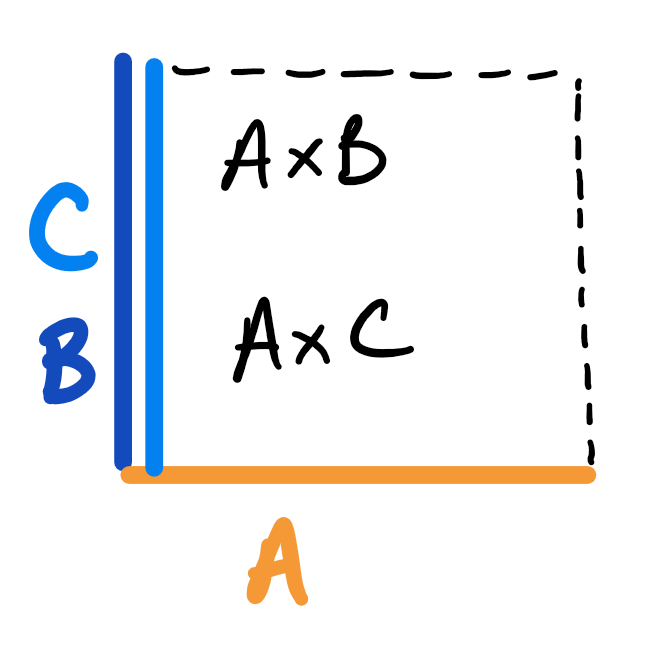
\includegraphics{Discrete/cart_product.PNG}}

we see that if the area of $A \times B$ equals the area of $A \times C$, then it must be the case that $B=C.$

\end{flaw}

\clearpage
\subsection{Error classification}

%Provide a brief classification and explanation of the errors in the Flawed Proof \ref{flaw:proof1}. %change the label

There are several errors
% is only one error ... etc.
 in the Flawed Proof \ref{flaw:cart_product}. %change the label

 
 \begin{description}
 	\item[F-Eg:] Proof by picture/example.
 	\item[C-FS:] The statement in question is false.
 	\item[F-EO-FS:] False statement caused omission of majority of the proof (i.e. a counterexample).
 \end{description}

 
\subsubsection{Error codes}
\begin{itemize}
	\item 	Fundamental Proof by Example (F-Eg)
	\item   Content False Statement (C-FS)
	\item   Fundamental Error-caused Omission resulting from False Statement (F-EO-FS)
\end{itemize}
See Section \ref{sec-error} for more information about error classifications.

\clearpage
\subsection{Corrected proof}

The following is a corrected version of Flawed Proof \ref{flaw:cart_product}. %change the label

\begin{prf}{prf:cart_product} %change the label
This statement is false. Consider the following counterexample. Let $A = \varnothing, B = \{1\}$ and $C=\{1,2\}.$ Then $A \times B = \varnothing$ and $A \times C = \varnothing,$ but $B \neq C$ since $2 \in C$  and $2 \notin B.$
\end{prf} % MATH 271
% Author: Christian Bagshaw
% Date: 
% Lauren DeDieu, Jerrod M.~Smith, Kimberly Golubeva and Christian Bagshaw
% A Resource Bank for Writing Intensive Mathematics Courses
% This work is licensed under a  Creative Commons Attribution-NonCommercial-ShareAlike 4.0 International License
% http://creativecommons.org/licenses/by-nc-sa/4.0/
\section{Cartesian Product Set Equality Again}

\begin{xca}{xca:cart_productagain}
Prove or disprove the following statement. For all sets $A,B$ and $C$, if $A \times B = A \times C,$ then $B=C.$ 
\end{xca}

\begin{flaw}{flaw:cart_productagain} %change the label
The statement is false. We will consider some cases. 

If $A$ is empty, then $A \times B = \emptyset \times B = \emptyset$ and $A \times C = \emptyset \times C = \emptyset$ so $A \times B = A \times C$. 

If $A$ is non-empty, then let $B, C$ both be empty. Then $A \times B = A \times \emptyset = \emptyset$ and $A \times C = A \times \emptyset = \emptyset$, so $A \times B = A\times C$, and of course $B = C$. 
\end{flaw}

\clearpage
\subsection{Error classification}

%Provide a brief classification and explanation of the errors in the Flawed Proof \ref{flaw:proof1}. %change the label

There are several errors
% is only one error ... etc.
 in the Flawed Proof \ref{flaw:cart_productagain}. %change the label

 
 \begin{description}
 	\item[F-WM:] There is no need to consider cases nor deal with arbitrary sets; only a counter-example is needed. 
 \end{description}

 
\subsubsection{Error codes}
\begin{itemize}
	\item 	Fundamental Wrong Method
\end{itemize}
See Section \ref{sec-error} for more information about error classifications.

\clearpage
\subsection{Corrected proof}

The following is a corrected version of Flawed Proof \ref{flaw:cart_productagain}. %change the label

\begin{prf}{prf:cart_productagain} %change the label
This statement is false. Consider the following counterexample. Let $A = \varnothing, B = \{1\}$ and $C=\{1,2\}.$ Then $A \times B = \varnothing$ and $A \times C = \varnothing,$ but $B \neq C$ since $2 \in C$  and $2 \notin B.$
\end{prf} % MATH 271
% Author: Christian Bagshaw
% Date: DD MMM 2020
% Lauren DeDieu, Jerrod M.~Smith, Kimberly Golubeva and Christian Bagshaw
% A Resource Bank for Writing Intensive Mathematics Courses
% This work is licensed under a  Creative Commons Attribution-NonCommercial-ShareAlike 4.0 International License
% http://creativecommons.org/licenses/by-nc-sa/4.0/
\section{Relations}

\begin{xca}[Almost Rational]{xca:almost_rational}
Let $\sim$ be a relation on $\mathbb{Z} \times \mathbb{Z}$ defined by $(a,b) \sim (a',b')$ iff $a'b = ab'$. Prove $\sim$ is not an equivalence relation on $\mathbb{Z} \times \mathbb{Z}$. 
\end{xca}

\begin{flaw}{flaw:almost_rational} %change the label
Need examples that contradict the definition of equivalence relation\\

Reflexive: $\checkmark$\\

Symmetric: $\checkmark$\\

Transitive: The error must be here. In class we did this but with $b \neq 0$ so it must have something to do with that. 


\end{flaw}

\clearpage
\subsection{Error classification}

%Provide a brief classification and explanation of the errors in the Flawed Proof \ref{flaw:proof1}. %change the label

There is one error
% is only one error ... etc.
 in the Flawed Proof \ref{flaw:almost_rational}. %change the label
 which we have classified using  the Coding Scheme Matrix in \cite[pp.~919]{Strickland_2016}. %% this reference may change if we modify the coding scheme matrix
 
 \begin{description}
    \item[SW] The flawed proof isnt a completed proof or even written as a proof - it is really just scratch work one might have been using in the process of discovering the proof. 

 	
 \end{description}

 
\subsubsection{Error codes}
\begin{itemize}
    \item Scratch Work (SW)
\end{itemize}
See Section \ref{sec-error} for more information about error classifications.

\clearpage
\subsection{Corrected proof}

The following is a corrected version of Flawed Proof \ref{flaw:almost_rational}. %change the label

\begin{prf}{prf:almost_rational} %change the label
We will disprove the statement by showing this relation is not transitive. Note that $(0,0)$, $(1,1)$, $(1,2) \in \mathbb{Z} \times \mathbb{Z}$. We can see that $(1,1) \sim (0,0)$ since $1 \cdot 0 = 0 \cdot 1$. Also we can see that $(0,0) \sim (1,2)$ since $0\cdot2 = 0\cdot1$. If this relation were transitive this would imply $(1,1) \sim (1,2)$ but $1\cdot 2 \neq 1 \cdot 1$ so this is not true. Thus this relation is not transitive. 
\end{prf} %
% Author: Kimberly Golubeva
% Date: 21 August 2020
% Lauren DeDieu, Jerrod M.~Smith, Kimberly Golubeva and Christian Bagshaw
% A Resource Bank for Writing Intensive Mathematics Courses
% This work is licensed under a  Creative Commons Attribution-NonCommercial-ShareAlike 4.0 International License
% http://creativecommons.org/licenses/by-nc-sa/4.0/
\section{Constructing Rationals from Integers}

\begin{xca}{xca:rat_from_int}
Let $\sim$ be the equivalence relation on $\Z \times \Z^\times$ given by,
$$(a,b) \sim (c,d) \text{ if } ad = bc\;.$$

Prove or disprove the statement,

$$(4,6) \sim (48,72)\;.$$
\end{xca}

\begin{flaw}{flaw:rat_from_int} %change the label
Yes, this statement is true since,

$$\frac46 = \frac23 = \frac{48}{72}\;.$$
\end{flaw}

\clearpage
\subsection{Error classification}

%Provide a brief classification and explanation of the errors in the Flawed Proof \ref{flaw:proof1}. %change the label

There are several errors
% is only one error ... etc.
 in the Flawed Proof \ref{flaw:rat_from_int}. %change the label

 
 \begin{description}
 	\item[F-A:] The entire result is asserted by stating that 
 	$$\frac46 = \frac23 = \frac{48}{72}\;.$$
 	That is, $ad = bc$ is asserted. 
 	\item[C-VG:] Misuse/misunderstanding of the required equivalence relation.
 \end{description}

 
\subsubsection{Error codes}
\begin{itemize}
	\item 	Fundamental Assertion (F-A)
	\item   Content Vocabulary and Grammar (C-VG)
\end{itemize}
See Section \ref{sec-error} for more information about error classifications.

\clearpage
\subsection{Corrected proof}

The following is a corrected version of Flawed Proof \ref{flaw:rat_from_int}. %change the label

\begin{prf}{prf:rat_from_int} %change the label
This statement is true. Recall that we can construct $\mathbb{Q}$ from $\mathbb{Z}$ using the equivalence relation on $\Z \times \Z^\times$ given by,
$$(a,b) \sim (c,d) \text{ if } ad = bc\;.$$
In our case, we have that $a = 4, \;b=6, \;c=48$ and $d=72.$ Then,
$$4(72) = 288 = 6(48)\;,$$
which implies that $(4,6) \sim (48,72).$
\end{prf}
 %MATH 273
% Author: Christian Bagshaw
% Date: August 2020
% Lauren DeDieu, Jerrod M.~Smith, Kimberly Golubeva and Christian Bagshaw
% A Resource Bank for Writing Intensive Mathematics Courses
% This work is licensed under a  Creative Commons Attribution-NonCommercial-ShareAlike 4.0 International License
% http://creativecommons.org/licenses/by-nc-sa/4.0/
\section{Counting Subsets}

\begin{xca}[Subsets containing even numbers]{xca:subset_counting}
Let $n \geq 3$ be an integer, let $N = \{1, 2, ..., n\}$. Express the number of subsets of $N$ containing at least one even number in terms of $n$. 
\end{xca}

\begin{flaw}{flaw:subset_counting} %change the label
If it has to contain an even number, then it is a subset of $\{2, 4, ..., n\}$ (the set of even numbers less than or equal to $n$). This set has $n/2$ elements. So the number of subsets of this set is $2^{n/2}$. 
\end{flaw}

\clearpage
\subsection{Error classification}

%Provide a brief classification and explanation of the errors in the Flawed Proof \ref{flaw:proof1}. %change the label

There are multiple errors
% is only one error ... etc.
 in the Flawed Proof \ref{flaw:subset_counting}
 
 \begin{description}
    \item[C-FI] ``it has to contain an even number'' does not imply  ``it is a subset of $\{2,4,...,n\}$''. 
    \item[C-FS] The set $\{2,3,...,n\}$ is not the set of even numbers less than or equal to $n$ if $n$ is odd. \item[C-FS] The set $\{2,4,...,n\}$ does not have $n/2$ elements if $n$ is odd. 

 	
 \end{description}

 
\subsubsection{Error codes}
\begin{itemize}
    \item Content False Implication (C-FI)
    \item Content False Statement (C-FS)
\end{itemize}
See Section \ref{sec-error} for more information about error classifications.

\clearpage
\subsection{Corrected proof}

The following is a corrected version of Flawed Proof \ref{flaw:subset_counting}. %change the label

\begin{prf}{prf:proof1} %change the label
Firstly, we know the total number of subsets of $N$ is $2^n$. A subset that contains no even numbers is a subset of $O = \{1,3,...,n\}$ if $n$ is odd or $O = \{1,3,...,n-1\}$ if $n$ is even. The size of $O$ is $n/2$ if $n$ is even, or $\ceil{n/2}$ if $n$ is odd. Either way, we can say the size of $O$ is $\ceil{n/2}$. Thus, the number of subsets of $O$ is $2^{\ceil{n/2}}$. Therefore, the number of subsets of $N$ containing at least one even number would be $2^n - 2^{\ceil{n/2}}$. 
\end{prf} %MATH 271
% Author: Kimberly Golubeva
% Date: 25 August 2020
% Lauren DeDieu, Jerrod M.~Smith, Kimberly Golubeva and Christian Bagshaw
% A Resource Bank for Writing Intensive Mathematics Courses
% This work is licensed under a  Creative Commons Attribution-NonCommercial-ShareAlike 4.0 International License
% http://creativecommons.org/licenses/by-nc-sa/4.0/
\section{Card Combinations}

\begin{xca}{xca:card_combo}
In a standard deck of $52$ cards, how many different $5$ card hands can be drawn?  
\end{xca}

\begin{flaw}{flaw:card_combo} %change the label
$52 \times 51 \times 50 \times 49 \times 48\;.$
\end{flaw}

\clearpage
\subsection{Error classification}

%Provide a brief classification and explanation of the errors in the Flawed Proof \ref{flaw:proof1}. %change the label

There are several errors
%is only one error
 in the Flawed Proof \ref{flaw:card_combo}. %change the label

 
 \begin{description}
 	\item[F-WM:] Used incorrect probability method. More specifically, the answer to the exercise requires the concept of combinations. 
 	\item[N-VG:] No explanation of chosen method provided. 
 \end{description}

 
\subsubsection{Error codes}
\begin{itemize}
	\item 	Fundamental Wrong Method (F-WM)
	\item   Novice Vocabulary and Grammar (N-VG)
\end{itemize}
See Section \ref{sec-error} for more information about error classifications.

\clearpage
\subsection{Corrected proof}

The following is a corrected version of Flawed Proof \ref{flaw:card_combo}. %change the label

\begin{prf}{prf:card_combo} %change the label
Since we need to choose $5$ objects from a total number of $52,$ we obtain the following combination,
$$\binom {52}{5}=\frac{52 \times 51 \times 50 \times 49 \times 48}{5 \times 4 \times 3 \times 2 \times 1}\;.$$
\end{prf} %MATH 271
% Author: Kimberly Golubeva
% Date: 7 September 2020
% Lauren DeDieu, Jerrod M.~Smith, Kimberly Golubeva and Christian Bagshaw
% A Resource Bank for Writing Intensive Mathematics Courses
% This work is licensed under a  Creative Commons Attribution-NonCommercial-ShareAlike 4.0 International License
% http://creativecommons.org/licenses/by-nc-sa/4.0/
\section{Conditional Probability}

\begin{xca}{xca:condish_coins}
Suppose that two coins are tossed. What is the probability of observing exactly two heads given that at least one head is observed?  
\end{xca}

\begin{flaw}{flaw:condish_coins} %change the label
Let $A$ denote the outcome of observing exactly two heads and $B$ denote the outcome of observing at least one head. We want to find $P(A|B).$ Then,
\begin{align*}
    P(A|B) &= \frac{P(A \cup B)}{P(B)} \\
    &= \frac{n(A \cup B)}{n(B)} \\
    &= \frac{3}{3} \\
    &= 1\;.
\end{align*}
\end{flaw}

\clearpage
\subsection{Error classification}

%Provide a brief classification and explanation of the errors in the Flawed Proof \ref{flaw:proof1}. %change the label

There %are several errors
 is only one error % ... etc.
 in the Flawed Proof \ref{flaw:condish_coins}. %change the label

 
 \begin{description}
 	\item[C-MT:] The formula for conditional probability is given by $$P(A|B) = \frac{P(A \cap B)}{P(B)}\;,$$ not $$P(A|B) = \frac{P(A \cup B)}{P(B)}\;.$$
 \end{description}

 
\subsubsection{Error codes}
\begin{itemize}
	\item 	Content Vocabulary and Grammar (C-VG)
\end{itemize}
See Section \ref{sec-error} for more information about error classifications.

\clearpage
\subsection{Corrected proof}

The following is a corrected version of Flawed Proof \ref{flaw:condish_coins}. %change the label

\begin{prf}{prf:condish_coins} %change the label
Let $A$ denote the outcome of observing exactly two heads and $B$ denote the outcome of observing at least one head. We want to find $P(A|B).$ Then,
\begin{align*}
    P(A|B) &= \frac{P(A \cap B)}{P(B)} \\
    &= \frac{n(A \cap B)}{n(B)} \\
    &= \frac{1}{3}\;.
\end{align*}
\end{prf}
 %MATH 271
% Author: Kimberly Golubeva
% Date: 14 September 2020
% Lauren DeDieu, Jerrod M.~Smith, Kimberly Golubeva and Christian Bagshaw
% A Resource Bank for Writing Intensive Mathematics Courses
% This work is licensed under a  Creative Commons Attribution-NonCommercial-ShareAlike 4.0 International License
% http://creativecommons.org/licenses/by-nc-sa/4.0/
\section{Properties of Functions: One-to-one and Onto}

\begin{xca}{xca:onetoone_notonto}
Consider the function $f: \Z \rightarrow \Z$ defined as
$$f(x) = 2x+1\;.$$
Is this function one-to-one? Is it onto? Prove or disprove. 
\end{xca}

\begin{flaw}{flaw:onetoone_notonto} %change the label
This function is one-to-one. Let $a,b \in \Z.$ Suppose that $f(a)=f(b).$ Then,
\begin{align*}
2a + 1 &= 2b + 1 \\
2a &= 2b \\
a &= b\;.
\end{align*}
Thus, $f$ is one-to-one. \\

This function is onto. Let $y \in \Z$. We want to prove that $f(x)=2x+1=y$. Isolating for $x$, we have that $x= \frac{y - 1}{2}$. So choose $x=\frac{y - 1}{2}$. Then $f(x)$ will always equal $y$. Thus, for all $x \in \Z, f(x)= y$ and so $f$ is onto.
\end{flaw}

\clearpage
\subsection{Error classification}

%Provide a brief classification and explanation of the errors in the Flawed Proof \ref{flaw:proof1}. %change the label

There are several errors
% is only one error ... etc.
 in the Flawed Proof \ref{flaw:onetoone_notonto}. %change the label

 
 \begin{description}
 	\item[F-WP:] This proof would be correct if the function was defined on a different domain and codomain. In particular, the function $f$ is both one-to-one and onto when $f: \R \rightarrow \R.$
 	\item[F-FS:] It is not true that $x=\frac{y - 1}{2}$ will always be an integer. 
 \end{description}

 
\subsubsection{Error codes}
\begin{itemize}
	\item 	Fundamental Wrong Problem (F-WP)
	\item   Fundamental False Statement (F-FS)
\end{itemize}
See Section \ref{sec-error} for more information about error classifications.

\clearpage
\subsection{Corrected proof}

The following is a corrected version of Flawed Proof \ref{flaw:onetoone_notonto}. %change the label

\begin{prf}{prf:onetoone_notonto} %change the label
This function is one-to-one. Let $a,b \in \Z.$ Suppose that $f(a)=f(b).$ Then,
\begin{align*}
2a + 1 &= 2b + 1 \\
2a &= 2b \\
a &= b\;.
\end{align*}
Thus, $f$ is one-to-one. \\

This function is not onto. Consider the following counterexample. Choose $y =0$, and assume that there exists $x \in \Z$ such that $f(x)=y.$ Then $f(x)=0 = 2x+1$, which means that $x = \frac{-1}{2}.$ But this is a contradiction since $x = -\frac{1}{2} \notin \Z.$ Thus, for all $x \in \Z, f(x) \neq y$ and so $f$ is not onto.
\end{prf}
 %MATH 271
% Author: Kimberly Golubeva
% Date: 21 September 2020
% Lauren DeDieu, Jerrod M.~Smith, Kimberly Golubeva and Christian Bagshaw
% A Resource Bank for Writing Intensive Mathematics Courses
% This work is licensed under a  Creative Commons Attribution-NonCommercial-ShareAlike 4.0 International License
% http://creativecommons.org/licenses/by-nc-sa/4.0/
\section{The Graph of a Matrix}

\begin{xca}{xca:matrix_graf}
Draw a graph, $G$, associated to the matrix

$$\begin{pmatrix}
0 & 1 & 1 & 1 & 1 \\
1 & 0 & 1 & 0 & 0 \\
1 & 1 & 0 & 1 & 0 \\
1 & 0 & 1 & 0 & 1 \\
1 & 0 & 0 & 1 & 0
\end{pmatrix}\;.$$
\end{xca}

\begin{flaw}{flaw:matrix_graf} %change the label
\center{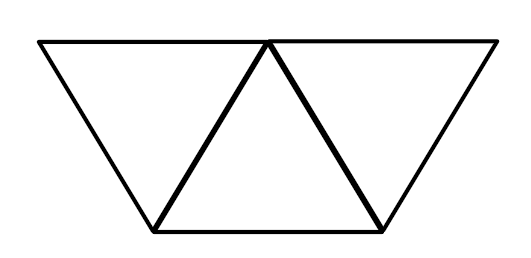
\includegraphics{Discrete/matrix_graf_incorrect.PNG}}
\end{flaw}

\clearpage
\subsection{Error classification}

%Provide a brief classification and explanation of the errors in the Flawed Proof \ref{flaw:proof1}. %change the label

There are several errors
% is only one error ... etc.
 in the Flawed Proof \ref{flaw:matrix_graf}. %change the label

 
 \begin{description}
 	\item[N-N:] The vertices $v_1, ..., v_5$ are not labeled, which makes it difficult to interpret the graph. 
 	\item[N-VG:] There are no explanations provided; more detail is required. 
 \end{description}

 
\subsubsection{Error codes}
\begin{itemize}
	\item 	Novice Notation (N-N)
	\item   Novice Vocabulary and Grammar (N-VG)
\end{itemize}
See Section \ref{sec-error} for more information about error classifications.

\clearpage
\subsection{Corrected proof}

The following is a corrected version of Flawed Proof \ref{flaw:matrix_graf}. %change the label

\begin{prf}{prf:matrix_graf} %change the label
\center{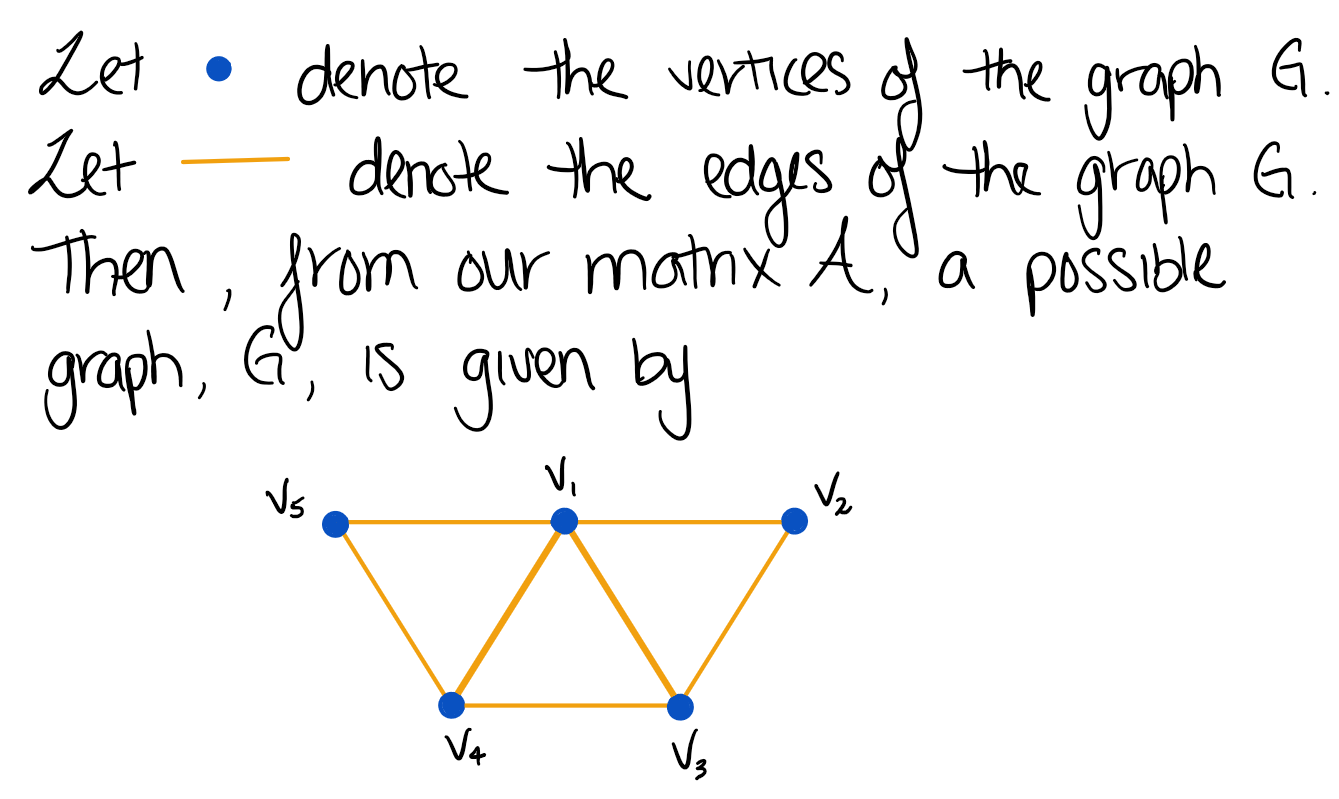
\includegraphics{Discrete/matrix_graf_correct.PNG}}
\end{prf} %MATH 271
% Author: Kimberly Golubeva
% Date: 28 September 2020
% Lauren DeDieu, Jerrod M.~Smith, Kimberly Golubeva and Christian Bagshaw
% A Resource Bank for Writing Intensive Mathematics Courses
% This work is licensed under a  Creative Commons Attribution-NonCommercial-ShareAlike 4.0 International License
% http://creativecommons.org/licenses/by-nc-sa/4.0/
\section{Addition and Multiplication of Congruence Relations}

\begin{xca}{xca:cong_add_mult}
Prove that if $a \equiv b\;(mod\;n)$ and $c \equiv d \;(mod\;n)$, then
\begin{enumerate}
    \item $(a+c) \equiv (b+d) \;(mod\;n)$\;,
    \item $ac \equiv bd \;(mod\;n)$\;.
\end{enumerate}
\end{xca}

\begin{flaw}{flaw:cong_add_mult} %change the label
Suppose that $a \equiv b\;(mod\;n)$ and $c \equiv d \;(mod\;n)$\;. By the definition of congruence, there exists integers $m$ and $k$ such that 
$$a-b = mn \quad \text{and} \quad c-d = kn\;.$$

We have
\begin{align*}
    (a+c) - (b+d) &= n(m+k) \\
    a-b+c-d &= n(m+k) \\
\end{align*}
which implies that $(a+c) \equiv (b+d)\; mod\;(n)\;.$ \\

We have
\begin{align*}
    ac - bd &=n(cm + bk), \\
    &= c(a-b) + b(c-d) \\
\end{align*}
which implies that $ac \equiv bd \;(mod\;n)$\;.

\end{flaw}

\clearpage
\subsection{Error classification}

%Provide a brief classification and explanation of the errors in the Flawed Proof \ref{flaw:proof1}. %change the label

There are several errors
% is only one error ... etc.
 in the Flawed Proof \ref{flaw:cong_add_mult}. %change the label

 
 \begin{description}
 	\item[C-Cir:] Both portions of the proof use the conclusion in the course of the proof. In particular, the conclusions $(a+c) - (b+d) = n(m+k)$ and $ac - bd =n(cm + bk)$ are assumed at the beginning of the proof. 
 	\item[C-EO-Cir:] Many of the important justification steps are omitted due to the arguments being circular. 
 	\item[F-A:] The results are asserted as there are no justifications for the conclusions reached. 
 \end{description}

 
\subsubsection{Error codes}
\begin{itemize}
	\item 	Content Circular Argument (C-Cir)
	\item   Content Error-Caused Omission due to Circular Argument (C-EO-Cir)
	\item   Fundamental Assertion (F-A)
\end{itemize}
See Section \ref{sec-error} for more information about error classifications.

\clearpage
\subsection{Corrected proof}

The following is a corrected version of Flawed Proof \ref{flaw:cong_add_mult}. %change the label

\begin{prf}{prf:cong_add_mult} %change the label
Suppose that $a \equiv b\;(mod\;n)$ and $c \equiv d \;(mod\;n)$\;. By the definition of congruence, there exists integers $m$ and $k$ such that 
$$a-b = mn \quad \text{and} \quad c-d = kn\;.$$

\noindent First we prove that  $(a+c) \equiv (b+d) \;(mod\;n)$\;.\\

We have
\begin{align*}
    a-b+c-d &= n(m+k) \\
    (a+c) - (b+d) &= n(m+k)\;,
\end{align*}
and so $n \vert (a+c) - (b+d)$ which implies that     $(a+c) \equiv (b+d)\; mod\;(n)\;.$ \\

\noindent Next, we prove that $ac \equiv bd \;(mod\;n)$\;. Here, we use that fact that $-bc + bc = 0.$\\

We have
\begin{align*}
    ac - bd &= ac + 0 -bd \\
    &= ac + (-bc + bc) - bd \\
    &= c(a-b) + b(c-d) \\
    &=c(mn) + b(kn) \\
    &=n(cm + bk)\;, 
\end{align*}
and so $n \vert (ac-bd)$ which implies that $ac \equiv bd \;(mod\;n)$\;.

\end{prf}
 %MATH 271
% Author: Christian Bagshaw
% Date: September 2020
% Lauren DeDieu, Jerrod M.~Smith, Kimberly Golubeva and Christian Bagshaw
% A Resource Bank for Writing Intensive Mathematics Courses
% This work is licensed under a  Creative Commons Attribution-NonCommercial-ShareAlike 4.0 International License
% http://creativecommons.org/licenses/by-nc-sa/4.0/
\section{Bayes Theorem}

\begin{xca}[Proof of Bayes Theorem]{xca:bayes}
Let $A$ and $B$ be two events. Recall that $P(A\cap B) = P(A)P(B|A)$. Prove that
$$P(A|B) = P(A)\frac{P(B|A)}{P(B)} $$
\end{xca}

\begin{flaw}{flaw:bayes} %change the label
The information given that $P(A\cap B) = P(A)P(B|A)$ is obviously a red herring because the thing we are trying to show doesn't use intersections. It is obvious that $P(B)P(A|B) = P(A)P(B|A)$ because one side is just rearranging the other side. Now manipulating that equation means that obviously $$P(A|B) = P(A)\frac{P(B|A)}{P(B)}$$ like we wanted. 
\end{flaw}

\clearpage
\subsection{Error classification}

%Provide a brief classification and explanation of the errors in the Flawed Proof \ref{flaw:proof1}. %change the label

There is only one error
% is only one error ... etc.
 in the Flawed Proof \ref{flaw:bayes}. 
 
 \begin{description}
    \item[F-A] The assertion that $P(B)P(A|B) = P(A)P(B|A)$ is at the heart of the proof and needs an explanation.



 	
 \end{description}

 
\subsubsection{Error codes}
\begin{itemize}
    \item Fundamental Assertion (F-A)
\end{itemize}
See Section \ref{sec-error} for more information about error classifications.

\clearpage
\subsection{Corrected proof}

The following is a corrected version of Flawed Proof \ref{flaw:bayes}. %change the label

\begin{prf}{prf:bayes} %change the label
We were given that $P(A\cap B) = P(A)P(B|A)$. But note that in an intersection, $A$ and $B$ are interchangable. So we can also write $P(A\cap B) = P(B\cap A) = P(B)P(A|B)$. This means $P(B)P(A|B) = P(A)P(B|A)$. Rearranging this means 
$$P(A|B) = P(A)\frac{P(B|A)}{P(B)}$$. 
\end{prf} %
% Author: Christian Bagshaw
% Date: Sept 2020
% Lauren DeDieu, Jerrod M.~Smith, Kimberly Golubeva and Christian Bagshaw
% A Resource Bank for Writing Intensive Mathematics Courses
% This work is licensed under a  Creative Commons Attribution-NonCommercial-ShareAlike 4.0 International License
% http://creativecommons.org/licenses/by-nc-sa/4.0/
\section{One-to-one Functions}

\begin{xca}[One-to-one from. $\mathbb{Z}$ to $\mathbb{N}$]{xca:z_to_n}
Find a function $f:\mathbb{Z} \to \mathbb{N}$ that is one-to-one, and prove that it is one-to-one. 
\end{xca}

\begin{flaw}{flaw:z_to_n} %change the label
Let $f(n) = n$. Then this is one-to-one ( because we did this in class) and it satisfies the things being asked. 
\end{flaw}

\clearpage
\subsection{Error classification}

%Provide a brief classification and explanation of the errors in the Flawed Proof \ref{flaw:proof1}. %change the label

There is only one error
% is only one error ... etc.
 in the Flawed Proof \ref{flaw:z_to_n}. 
 
 \begin{description}
    \item[F-FS] $f(n) = n$ does not work as this is not a well-defined function from $\mathbb{Z}$ to $\mathbb{N}$. 



 	
 \end{description}

 
\subsubsection{Error codes}
\begin{itemize}
    \item Fundamental False Statement (F-FS)
\end{itemize}
See Section \ref{sec-error} for more information about error classifications.

\clearpage
\subsection{Corrected proof}

The following is a corrected version of Flawed Proof \ref{flaw:z_to_n}. %change the label

\begin{prf}{prf:z_to_n} %change the label
Define $f: \mathbb{Z} \to \mathbb{N}$ as follows:
$$f(n) = \begin{cases}
2|n| + 1 & x < 0\\
2n & x \geq 0
\end{cases}
$$
Now to show that this is one-to-one, let $a,b \in \mathbb{Z}$ such that $f(a) = f(b)$. Now firstly note that under $f$, all negative integers get mapped to odd integers and all non-negative integers get mapped to even integers. So if $f(a) = f(b)$ then $a,b$ are either both negative or both non-negative. We will consider each case
\begin{itemize}
    \item If $a,b < 0$ then $f(a) = f(b)$ means $2|a| + 1 = 2|b| + 1$, which means $|a| = |b|$. Since both are negative, this means $a=b$. 
    \item If $a,b > 0$ then $f(a) = f(b)$ means $2a = 2b$ , which means $a=b$.
\end{itemize}
Therefore $f(a) = f(b)$ implies $a=b$, so $f$ is one-to-one. 
\end{prf} %
% Author: Christian Bagshaw
% Date: DD MMM 2020
% Lauren DeDieu, Jerrod M.~Smith, Kimberly Golubeva and Christian Bagshaw
% A Resource Bank for Writing Intensive Mathematics Courses
% This work is licensed under a  Creative Commons Attribution-NonCommercial-ShareAlike 4.0 International License
% http://creativecommons.org/licenses/by-nc-sa/4.0/
\section{Relations}

\begin{xca}[Transitive Relation]{xca:order_relation}
For this question, $0 \notin \mathbb{N}$. Let $<$ be the relation on $\mathbb{N}$ (the natural numbers) defined by 
$$\text{for all} \: m,n \in \mathbb{N}, \: n < m  \text{ iff there exists some } p \in \mathbb{N} \text{ such that } n+p = m $$
Prove that this is a transitive relation, but not a symmetric relation. 
\end{xca}

\begin{flaw}{flaw:order_relation} %change the label
Let $a<b$ and $b<c$. Then of course $a<c$ so this is transitive.\\

\noindent I can show this isnt symmetric because its not possible for $a<b$ and $b<a$. 
\end{flaw}

\clearpage
\subsection{Error classification}

%Provide a brief classification and explanation of the errors in the Flawed Proof \ref{flaw:proof1}. %change the label

There is only one error
% is only one error ... etc.
 in the Flawed Proof \ref{flaw:order_relation}. %change the label

 
 \begin{description}
    \item[F-A] Entire result was asserted. \item[N-VG] Use of the first person pronoun ``I'' is typically bad form in a mathematical proof.
 	\item[C-N] $a,b$ and $c$ are not defined. 
 \end{description}

 
\subsubsection{Error codes}
\begin{itemize}
	\item Fundamental Assertion (F-A)
	\item Novice Vocabulary and Grammar (N-VG)
	\item Content Notation (C-N)
\end{itemize}
See Section \ref{sec-error} for more information about error classifications.

\clearpage
\subsection{Corrected proof}

The following is a corrected version of Flawed Proof \ref{flaw:order_relation}. %change the label

\begin{prf}{prf:order_relation} %change the label
Let $a,b,c \in \mathbb{N}$ such that $a<b$ and $b < c$. We need to show this implies $a < c$. Since $a<b$, there exists some $p \in \mathbb{N}$ such that $a+p = b$. Also since $b<c$ there exists some $q \in \mathbb{N}$ such that $b + q = c$. Now substituting gives $a + p + q = c$. Now since $p,q \in \mathbb{N}$, $p+q \in \mathbb{N}$. So let $r = p+q$. Then $a+r = c$, so $a < c$. \\

To show this is not a symmetric relation, suppose there exists $a,b \in \mathbb{N}$ such that $a<b$ and $b<a$. Then there exists natural numbers $p,q$ such that $a+q = b$ and $b+p = a$. Substituting gives $b+p+q = b$, or that $p+q = 0$. This is not possible for natural numbers $p,q$. Therefore, this relation is not symmetric. 
\end{prf} %
% Author: Christian Bagshaw
% Date: DD MMM 2020
% Lauren DeDieu, Jerrod M.~Smith, Kimberly Golubeva and Christian Bagshaw
% A Resource Bank for Writing Intensive Mathematics Courses
% This work is licensed under a  Creative Commons Attribution-NonCommercial-ShareAlike 4.0 International License
% http://creativecommons.org/licenses/by-nc-sa/4.0/
\section{Equivalence Relations}

\begin{xca}[Modular Congruence is Transitive]{xca:equiv_modular}
Prove that modular congruence is transitive; that is, for integers $a,b,c,n$, prove that if $a \equiv b \mod n$ and $b \equiv c \mod n$, then $a \equiv c \mod n$. 

\end{xca}

\begin{flaw}{flaw:equiv_modular} %change the label

Since $a \equiv b \mod n$, then $a - b = nk$. Now if we let $n = c-b$ and $k=1$, then $a-b = c-b = nk$, or $a-c = nk$. So $a\equiv c \mod n$. 
\end{flaw}

\clearpage
\subsection{Error classification}

%Provide a brief classification and explanation of the errors in the Flawed Proof \ref{flaw:proof1}. %change the label

There are several errors
% is only one error ... etc.
 in the Flawed Proof \ref{flaw:equiv_modular}. 
 
 \begin{description}
    \item[N-N] $k$ is not defined. 
    \item[C-Eg] The statement needs to be proven for all $n$, but the proof attempts to prove the statement for a specific $n$
    \item[F-FI] That $a-b = c-b = nk$ implies $a-c = nk$ is false. 

 	
 \end{description}

 
\subsubsection{Error codes}
\begin{itemize}
    \item Novice Notation (N-N)
	\item Content Proof by Example (C-Eg)
	\item Fundamental False Implication (F-FI)
\end{itemize}
See Section \ref{sec-error} for more information about error classifications.

\clearpage
\subsection{Corrected proof}

The following is a corrected version of Flawed Proof \ref{flaw:equiv_modular}. %change the label

\begin{prf}{prf:equiv_modular} %change the label
For integers $a,b,c,n$ suppose that $a \equiv b \mod n$ and $b \equiv c \mod n$. This means there exists integer $k, l$ such that $a-b = nk$ and $b-c = nl$. Solving for $b$ in the second equation gives $b = nl + c$. Substituting into the second equation means $a - nl - c = nk$, so $a-c = nl + nk = n(l + k)$. Thus $n$ divides $a-c$, so by definition $a\equiv c \mod n$. 
\end{prf} %
% Author: Kimberly Golubeva
% Date: 20 April 2020
% Lauren DeDieu, Jerrod M.~Smith, Kimberly Golubeva and Christian Bagshaw
% A Resource Bank for Writing Intensive Mathematics Courses
% This work is licensed under a  Creative Commons Attribution-NonCommercial-ShareAlike 4.0 International License
% http://creativecommons.org/licenses/by-nc-sa/4.0/
\section{Set Containment Version Two}

\begin{xca}{xca:set_containment_subtle}
Prove or disprove the following statement. For all sets $A, B$ and $C$,
$$A \cap \left(B \cup C \right) \subseteq \left(A \cap B\right) \cup C\;.$$
\end{xca}

\begin{flaw}{flaw:set_containment_subtle} %change the label
Suppose $A, B$ and $C$ are sets. Suppose that $x \in A \cap \left(B \cup C \right).$ Then $x\in A$ and $x \in B \cup C.$ Since $x \in B \cup C,$ we can arbitrarily choose to consider $x \in B$. 
Suppose that $x \in B$. Then $x \in A$ and $x \in B$, so $x \in A \cap B$. Thus, $x \in \left(A \cap B\right) \cup C.$ Therefore, We can conclude that $$A \cap \left(B \cup C \right) \subseteq \left(A \cap B\right) \cup C\;.$$
\end{flaw}

\clearpage
\subsection{Error classification}

%Provide a brief classification and explanation of the errors in the Flawed Proof \ref{flaw:proof1}. %change the label

There are several errors
% is only one error ... etc.
 in the Flawed Proof \ref{flaw:set_containment_subtle}. %change the label

 
 \begin{description}
  	\item[C-VG: ] Misunderstanding of the definition of the union operation, evidenced by the statement: `Since $x \in B \cup C,$ we can arbitrarily choose to consider $x \in B$.' Both cases must be considered.   
 	\item[C-OS: ] The case where $x \in C$ is omitted. 
 \end{description}

 
\subsubsection{Error codes}
\begin{itemize}
	\item 	Content Vocabulary and Grammar (C-VG)
	\item   Content Omitted Section (C-OS)
\end{itemize}
See Section \ref{sec-error} for more information about error classifications.

\clearpage
\subsection{Corrected proof}

The following is a corrected version of Flawed Proof \ref{flaw:set_containment_subtle}. %change the label

\begin{prf}{prf:set_containment_subtle} %change the label
Suppose $A, B$ and $C$ are sets. Suppose that $x \in A \cap \left(B \cup C \right).$ Then $x\in A$ and $x \in B \cup C.$ Since $x \in B \cup C,$ we know that $x \in B$ or $x \in C.$ Thus, we have two cases to consider: \\

\noindent \textbf{Case 1:} Suppose that $x \in B$. Then $x \in A$ and $x \in B$, so $x \in A \cap B$. Thus, $x \in \left(A \cap B\right) \cup C.$ \\
\textbf{Case 2:}  Suppose that $x \in C$. Since $x \in C,$ then $x \in \left(A \cap B\right) \cup C.$ \\

\noindent Thus, in both cases $x \in \left(A \cap B\right) \cup C.$ Therefore, We can conclude that $$A \cap \left(B \cup C \right) \subseteq \left(A \cap B\right) \cup C\;.$$
\end{prf}
 %MATH 271 %Added April 20 2021 
% Author: Kimberly Golubeva
% Date: 20 April 2020
% Lauren DeDieu, Jerrod M.~Smith, Kimberly Golubeva and Christian Bagshaw
% A Resource Bank for Writing Intensive Mathematics Courses
% This work is licensed under a  Creative Commons Attribution-NonCommercial-ShareAlike 4.0 International License
% http://creativecommons.org/licenses/by-nc-sa/4.0/
\section{Surjection}

\begin{xca}{xca:surjection_backwards}
Consider the function $f: \mathbb{R}- \{0\} \rightarrow \mathbb{R}-\{1\}$ defined by 
$$f(x) = \frac{x + 15}{x}\;.$$
Is $f$ surjective? Prove or disprove.
\end{xca}

\begin{flaw}{flaw:surjection_backwards} %change the label
Yes, $f$ is surjective since for all $y \in \mathbb{R}-\{1\}$, there exists an $x \in \mathbb{R}-\{0\}$ such that $y=f(x).$ Namely, 
\begin{align*}
    y =& f(x) \\
    y =& \frac{x+15}{x} \\
    yx =& x+15 \\
    yx - x =& 15 \\
    x(y-1) =& 15 \\
    x =& \frac{15}{y-1}\;.
\end{align*}
Thus, we can see that $f$ is surjective.
\end{flaw}

\clearpage
\subsection{Error classification}

%Provide a brief classification and explanation of the errors in the Flawed Proof \ref{flaw:proof1}. %change the label

There are several errors
% is only one error ... etc.
 in the Flawed Proof \ref{flaw:surjection_backwards}. %change the label

 
 \begin{description}
    \item[EO-F-A: ] Although the method of finding $x$ is correct, the entirety of the proof is omitted (that is, verifying that $f(x)=y$ with the particular $x$ that was calculated) due to the assumption that $y=f(x)$. 
 	\item[C-VG: ] Misunderstanding the definition of surjective. 
 \end{description}

 
\subsubsection{Error codes}
\begin{itemize}
	\item 	Error-Caused Omission Fundamental Assertion (EO-F-A)
	\item   Content Vocabulary and Grammar
\end{itemize}
See Section \ref{sec-error} for more information about error classifications.

\clearpage
\subsection{Corrected proof}

The following is a corrected version of Flawed Proof \ref{flaw:surjection_backwards}. %change the label

\begin{prf}{prf:surjection_backwards} %change the label
Yes, $f$ is surjective. To prove this, we begin by finding a suitable $x \in \mathbb{R}-\{0\}$:
\begin{align*}
    y =& f(x) \\
    y =& \frac{x+15}{x} \\
    yx =& x+15 \\
    yx - x =& 15 \\
    x(y-1) =& 15 \\
    x =& \frac{15}{y-1}\;.
\end{align*}
So choose $x= \frac{15}{y-1}$ with $x \in \mathbb{R}-\{0\}$. Then,

$$f \left (\frac{15}{y-1} \right ) = \frac{\frac{15}{y-1} + 15}{\frac{15}{y-1}} = \frac{15 + 15(y-1)}{15} = \frac{15+15y-15}{15} = y\;. $$

Thus, we can see that $f$ is surjective since for all $y \in \mathbb{R}-\{1\}$, there exists an $x \in \mathbb{R}-\{0\}$ such that $f(x)=y.$  
\end{prf} %MATH 271 %Added April 20 2021 
% Author: Kimberly Golubeva
% Date: 20 April 2020
% Lauren DeDieu, Jerrod M.~Smith, Kimberly Golubeva and Christian Bagshaw
% A Resource Bank for Writing Intensive Mathematics Courses
% This work is licensed under a  Creative Commons Attribution-NonCommercial-ShareAlike 4.0 International License
% http://creativecommons.org/licenses/by-nc-sa/4.0/
\section{Injection}

\begin{xca}{xca:injection_subtle}
Consider $f: \mathbb{R} \rightarrow \mathbb{R}$ and $g: \mathbb{Z} \rightarrow \mathbb{Z}$ where $f(x) = 3x-4$ and $g(n) = n^4$ for all $n \in \mathbb{Z}.$ Is $f$ injective? Is $g$ injective? Prove or disprove.
\end{xca}

\begin{flaw}{flaw:injection_subtle} %change the label
Yes, $f$ is injective. Suppose that $a, b \in \mathbb{R}$ and that $f(a) = f(b)$. Then:
\begin{align*}
    f(a) &= f(b) \\
    3a-4 &= 3b-4 \\
    3a &= 3b \\
    a &= b\;.
\end{align*}
Thus, $f$ is injective. 

Yes, $g$ is injective. Suppose that $a, b \in \mathbb{Z}$ and that $g(a) = g(b)$. Then:
\begin{align*}
    g(a) &= g(b) \\
    \sqrt[4]{a^4} &= \sqrt[4]{b^4} \\
    a &= b \;.
\end{align*}
Thus, $g$ is injective. 
\end{flaw}

\clearpage
\subsection{Error classification}

%Provide a brief classification and explanation of the errors in the Flawed Proof \ref{flaw:proof1}. %change the label

There is only one error
 in the Flawed Proof \ref{flaw:injection_subtle}. %change the label

 
 \begin{description}
 	\item[EO-C-FS] The entirely of the proof was omitted due to the false statement that $\sqrt[4]{a^4} = \sqrt[4]{b^4} \implies
    a = b.$ Namely, it was assumed that $a$ and $b$	are positive.
 \end{description}

 
\subsubsection{Error codes}
\begin{itemize}
	\item 	Error-cased Omission Content False Statement
\end{itemize}
See Section \ref{sec-error} for more information about error classifications.

\clearpage
\subsection{Corrected proof}

The following is a corrected version of Flawed Proof \ref{flaw:injection_subtle}. %change the label

\begin{prf}{prf:injection_subtle} %change the label
Yes, $f$ is injective. Suppose that $a, b \in \mathbb{R}$ and that $f(a) = f(b)$. Then:
\begin{align*}
    f(a) &= f(b) \\
    3a-4 &= 3b-4 \\
    3a &= 3b \\
    a &= b\;.
\end{align*}
Thus, $f$ is injective. 

No, $g$ is not injective. To prove this, we will consider the following counterexample. Let $a = 2$ and $b=-2$. Then:
\begin{align*}
    g(a) &= g(b) \\
    16 &= 16 \\
    2^4 &= (-2)^4\;,
\end{align*}
and so $g(a)=g(b)=16,$ but $a=2 \neq -2 = b$. Thus, $g$ is not injective. 
\end{prf}
 %MATH 271 %Added April 20 2021 


%----------------------CHAPTER SIX LINEAR ALGEBRA
\chapter{Linear Algebra}\label{ch-lin}
The material in this chapter is designed to fit within a typical second course in abstract linear algebra and is based on the material covered in MATH 311: Linear Methods {\rm{II}} at the University of Calgary.

Topics include: subspaces, span, linear independence, bases and dimension in finite dimensional real vector spaces; eigenvalues, eigenvectors and orthogonality  in $\R^n$, row and column spaces, the Rank-Nullity theorem, the Gram-Schmidt Algorithm,  similar matrices,  orthogonal diagonalization; linear transformations, kernel, image, injections and surjections, isomorphisms, inverses, the matrix of a linear transformation and change of basis.

The following topics, which may appear in your course, are omitted: complex vector spaces, inner products, positive definite matrices, canonical matrix forms (i.e., Jordan Canonical Form, etc.), infinite dimensional vector spaces, and many others.

%-----------------%-----------------
% Author: Christian Bagshaw
% Date: 21 August 2020
% Lauren DeDieu, Jerrod M.~Smith, Kimberly Golubeva and Christian Bagshaw
% A Resource Bank for Writing Intensive Mathematics Courses
% This work is licensed under a  Creative Commons Attribution-NonCommercial-ShareAlike 4.0 International License
% http://creativecommons.org/licenses/by-nc-sa/4.0/
\section{Skew-Symmetric Matrices}

\begin{xca}{xca:skewsymmat}
Decide whether the following statement is TRUE or FALSE. If it's true, then prove it. If it's false, then  find an explicit counterexample. \\

Every $2\times 2$ skew-symmetric matrix has a determinant of zero.
\end{xca}

\begin{flaw}{flaw:skewsymmat} %change the label
The statement is false. To see this, suppose we had a $2\times 2$ skew-symmetric matrix $A$. Then we can write $A = \begin{pmatrix}0 & a \\ -a & 0 \end{pmatrix}$ for some $a \in \mathbb{R}$. A simple computation gives $\det(A) = a^2$, and squares are always positive.
\end{flaw}

\clearpage
\subsection{Error classification}

%Provide a brief classification and explanation of the errors in the Flawed Proof \ref{flaw:proof1}. %change the label

There are several errors
% is only one error ... etc.
 in the Flawed Proof \ref{flaw:skewsymmat}. %change the label


 \begin{description}
 \item[WM] The student is trying to prove that the statement is always false, but the prompt says to find an explicit counterexample if the statement is false.
 \item[EO-(F-FS):] An explicit counterexample is omitted due to the false statement that $a^2$ is always positive.

 	\item[C-A:] The claim that every $2\times 2$ skew-symmetric matrix $A$ can be written in that specific form requires more justification.
 \end{description}


\subsubsection{Error codes}
\begin{itemize}
\item Wrong Method (WM)	
\item Error-caused Omission due to Fundamental False Statement (EO-(F-FS))
	\item Content Assertion (C-A)
\end{itemize}
See Section \ref{sec-error} for more information about error classifications.

\clearpage
\subsection{Corrected proof}

The following is a corrected version of Flawed Proof \ref{flaw:skewsymmat}. %change the label

\begin{prf}{prf:skewsymmat} %change the label
This statement is false. Indeed, consider $A = \begin{pmatrix}0 & 1 \\ -1 & 0 \end{pmatrix}$. This matrix $A$ is skew-symmetric since $A = -A^T$, but $\det(A) = 1 \neq 0$.
\end{prf}  %MATH 311
% Author: Christian Bagshaw
% Date: August 2020
% Lauren DeDieu, Jerrod M.~Smith, Kimberly Golubeva and Christian Bagshaw
% A Resource Bank for Writing Intensive Mathematics Courses
% This work is licensed under a  Creative Commons Attribution-NonCommercial-ShareAlike 4.0 International License
% http://creativecommons.org/licenses/by-nc-sa/4.0/
\section{Intersection of Subspaces}

\begin{xca}[Intersection of Subspaces]{xca:sub-intersect}
Let $V$ and $W$ be subspaces of $\mathbb{R}^n$. Prove that $V \cap W$ is a subspace of $\mathbb{R}^n$.
\end{xca}

\begin{flaw}{flaw:sub-intersect} %change the label
To show that $V\cap W$ is a subspace, we will show that it contains the zero vector, is closed under addition and is closed under scalar multiplication. \\

Firstly, since $V$ and $W$ are subspaces of $\mathbb{R}^n$, we know that $\bm{0} \in V$ and $\bm{0} \in W$. This means $\bm{0} \in V \cap W$. \\

Secondly, let $\bm{v}_1, \bm{v}_2 \in V \cap W$. Since $V$ and $W$ are subspaces this means $\bm{v}_1 + \bm{v}_2 \in V \cap W$. \\

Thirdly, let $\bm{v} \in V \cap W$ and $k \in \mathbb{R}$. Since $V$ and $W$ are subspaces this means $k\bm{v} \in V \cap W$. \\

\end{flaw}

\clearpage
\subsection{Error classification}

%Provide a brief classification and explanation of the errors in the Flawed Proof \ref{flaw:proof1}. %change the label

There are several errors
% is only one error ... etc.
 in the Flawed Proof \ref{flaw:sub-intersect}.

 \begin{description}
    \item[C-A]  The assertion ``let $\bm{v}_1, \bm{v}_2 \in V \cap W$. Since $V$ and $W$ are subspaces this means $\bm{v}_1 + \bm{v}_2 \in V \cap W$" is true, but has not been sufficiently proven.
    \item[C-A] The assertion ``let $\bm{v} \in V \cap W$ and $k \in \mathbb{R}$. Since $V$ and $W$ are subspaces this means $k\bm{v} \in V \cap W$" is true, but has not been sufficiently proven.
 	
 \end{description}


\subsubsection{Error codes}
\begin{itemize}
	\item 	Content Assertion (C-A)
\end{itemize}
See Section \ref{sec-error} for more information about error classifications.

\clearpage
\subsection{Corrected proof}

The following is a corrected version of Flawed Proof \ref{flaw:sub-intersect}. %change the label

\begin{prf}{prf:sub-intersect} %change the label
To show that $V\cap W$ is a subspace, we will show that it contains the zero vector, is closed under addition and is closed under scalar multiplication. \\

Firstly, since $V$ and $W$ are subspaces of $\mathbb{R}^n$, we know that $\bm{0} \in V$ and $\bm{0} \in W$. This means $\bm{0} \in V \cap W$. \\

Secondly, let $\bm{v}_1, \bm{v}_2 \in V \cap W$. This means $\bm{v}_1, \bm{v}_2 \in V$ and $\bm{v}_1, \bm{v}_2 \in W$. Since $V$ and $W$ are subspaces they are both closed under addition, so $\bm{v}_1 + \bm{v}_2 \in V$ and $\bm{v}_1 + \bm{v}_2 \in W$. This means $\bm{v}_1 + \bm{v}_2 \in V \cap W$. \\

Thirdly, suppose $\bm{v} \in V \cap W$. So $\bm{v} \in V$ and $\bm{v} \in W$. Let $k \in \mathbb{R}$. Since $V$ and $W$ are subspaces they are both closed under scalar multiplication, so $k\bm{v} \in V$ and $k\bm{v} \in W$. This means $k\bm{v} \in V \cap W$.
\end{prf}  %MATH 311
%Author: Kimberly Golubeva
%Date: July 14 2020
% Lauren DeDieu, Jerrod M.~Smith, Kimberly Golubeva and Christian Bagshaw
% A Resource Bank for Writing Intensive Mathematics Courses
% This work is licensed under a  Creative Commons Attribution-NonCommercial-ShareAlike 4.0 International License
% http://creativecommons.org/licenses/by-nc-sa/4.0/
\section{Sum of Subspaces}

\begin{xca}[]{xca:sumsubspaces}
Prove or disprove the following statement. If $V$ and $W$ are both subspaces of $\mathbb{R}^n$, then $V+W$ is also a subspace of $\mathbb{R}^n$.
\end{xca}

\begin{flaw}{flaw:sumsubspaces}
This statement is true. We will use the definition of a subspace to prove that $V+W$ is a subspace.

\begin{enumerate}
\item Contains $\vec{0}$: Take $\vec{0} \in V$ and $\vec{0} \in W$. Then $\vec{0} + \vec{0} = \vec{0} \in V + W.$
\item Closed Under Addition: Let $\vec{v} \in V$ and $\vec{w} \in W$. Then $\vec{v} + \vec{w} \in V+W$, which means that $V+W \in \mathbb{R}^n.$
\item Closed Under Scalar Multiplication: Let  $\vec{v} \in V+W$ and $w \in \mathbb{R}.$ Then $\vec{v}(w)= \vec{v}w \in V+W.$
\end{enumerate}
\end{flaw}

\clearpage
\subsection{Error classification}

%Provide a brief classification and explanation of the errors in the Flawed Proof \ref{flaw:proof1}. %change the label

There are several errors
% is only one error ... etc.
 in the Flawed Proof \ref{flaw:sumsubspaces}.

\begin{description}
 	\item[EO-(C-VG):] Misunderstanding what it means to be `closed' under addition and scalar multiplication leading to omission of major parts of the proof. Start with elements that are in $V+W$ and show that they are still in $V+W$ after these operations are performed.
 %	\item [F-A:] The `Closed Under Addition' and `Closed Under Scalar Multiplication' portions of the proof are asserted due to misunderstanding the notion of being `closed'. 	
 	\item[N-N:] To avoid confusing notation, choose a different letter for the scalar.

 \end{description}


\subsubsection{Error codes}
\begin{itemize}
	\item 	Error-Caused Omission due to Content Vocabulary $\&$ Grammar (EO-(C-VG))
	%\item   Fundamental Assertion (F-A)
	\item   Novice Notation (N-N)
\end{itemize}
See Section \ref{sec-error} for more information about error classifications.

\clearpage
\subsection{Corrected proof}

The following is a corrected version of Flawed Proof \ref{flaw:sumsubspaces}. %change the label

\begin{prf}{prf:sumsubspaces} %change the label
This statement is true. We will use the definition of a subspace to prove that $V+W$ is a subspace.

\begin{enumerate}
\item Contains $\vec{0}$: Since both $V$ and $W$ are subspaces, take $\vec{0} \in V$ and $\vec{0} \in W$. Then $\vec{0} + \vec{0} = \vec{0} \in V + W.$
\item Closed Under Addition: Let $\vec{x}, \vec{y} \in V+W$. By definition, there exists $\vec{v_1}, \vec{v_2} \in V$ and $\vec{w_1}, \vec{w_2} \in W$ such that $\vec{x} = \vec{v_1} +\vec{w_1}$ and $\vec{y} = \vec{v_2} +\vec{w_2}$. Then
$$\vec{x} + \vec{y} = (\vec{v_1} +\vec{w_1}) + (\vec{v_2} +\vec{w_2}) = (\vec{v_1} +\vec{v_2}) + (\vec{w_1} +\vec{w_2}).$$
Since $V$ is a subspace, it is closed under addition and so $(\vec{v_1} +\vec{v_2}) \in V$. Similarly, $(\vec{w_1} +\vec{w_2}) \in W$. This means that $(\vec{v_1} +\vec{v_2}) + (\vec{w_1} +\vec{w_2}) \in V + W$. Thus, $\vec{x} + \vec{y} \in V+W$ and so $V+W$ is closed under addition.
\item Closed Under Scalar Multiplication: Let  $\vec{x} \in V+W$ and $k \in \mathbb{R}.$ By definition, there exists $\vec{v} \in V$ and $\vec{w} \in W$ such that $\vec{x} = \vec{v} +\vec{w}$. Then
$$k\vec{x} = k(\vec{v} +\vec{w})= k\vec{v} + k\vec{w}.$$
Since $V$ is a subspace, it is closed under scalar multiplication and so $k\vec{v} \in V$. Similarly, $k\vec{w} \in W$. This means that $k\vec{v} + k\vec{w} \in V+W$. Thus, $k\vec{x} \in V+W$ and so $V+W$ is closed under scalar multiplication.
\end{enumerate}
\end{prf}
 %MATH 311
% Author: Lauren DeDieu
% Date: 10 July 2020
% Lauren DeDieu, Jerrod M.~Smith, Kimberly Golubeva and Christian Bagshaw
% A Resource Bank for Writing Intensive Mathematics Courses
% This work is licensed under a  Creative Commons Attribution-NonCommercial-ShareAlike 4.0 International License
% http://creativecommons.org/licenses/by-nc-sa/4.0/
\section{Subspaces and Nullspace}

\textbf{Subspace Test:} A set $U\subseteq\mathbb{R}^n$ is called a \textbf{subspace} of $\mathbb{R}^n$ if it satisfies the following:
\begin{itemize}
\item Zero Vector: $\vec{0}\in U$.
\item Closed Under Addition: $\vec{x},\vec{y}\in U \Rightarrow\vec{x}+\vec{y}\in U$.
\item Closed Under Scalar Multiplication: $\vec{x}\in U \Rightarrow k\vec{x}\in U \, \forall \, k\in\mathbb{R}$.
\end{itemize}

\begin{xca}{xca:lin-ind-col-sp}
Let $A$ be an $m\times n$ matrix. Prove that $\mathrm{null}(A)$ is a subspace of $\mathbb{R}^n$ by using the definition of a subspace (i.e. the Subspace Test).
\end{xca}

\begin{flaw}{flaw:lin_sub_v1}
\[\mathrm{null}(A)=\{\vec{x}\,|\,A\vec{x}=\vec{0}\}.\]

For a set to be a subspace 3 conditions must hold:

\begin{enumerate}
\item closed under addition
\item closed under multiplication
\item must contain $\vec{0}$
\end{enumerate}

Members of $\mathrm{nul}(A)$ will have $\mathrm{dim}(\mathrm{null}(A))=n$ since $A$ is an $m\times n$ matrix. \\

Thus ($\vec{x}+\vec{y})\in\mathbb{R}^n$ for any arbitrary $\vec{y}\in\mathbb{R}^n$ holds. \\

And $(k\vec{x})\in\mathbb{R}$ for any arbitrary scalar $\in\mathbb{R}$ holds. \\

And $\vec{x}=\vec{0}$ is implied by the line above where $k=0$.

\end{flaw}

\clearpage
\subsection{Error classification}

There are several errors in the Flawed Proof \ref{flaw:lin_sub_v1}.

\begin{description}
	\item[C-FI:] The matrix $A$ having size $m\times n$ does not imply $\mathrm{dim}(\mathrm{null}(A))=n$.
\item[EO-(C-VG):] Misunderstanding of what it means for a set to be closed under addition and closed under scalar multiplication leads to omission of major parts of the proof.
\item[C-A] Claiming closed under scalar multiplication implies contains the zero vector, but hasn't shown $\mathrm{null}(A)$ is nonempty.
\item[N-O] The variable $\vec{x}$ is not defined. 
\item[N-N] Using $\in$ in the middle of a sentence: ``for any arbitrary scalar $\in\mathbb{R}$''.
\item[N-FI] The claim $(k\vec{x})\in\mathbb{R}$ is false.
\item[WM] Not showing that the zero vector is contained in $\mathrm{null}(A)$ using the definition of a subspace as the prompt requires.
\end{description}

\subsubsection{Error codes}
\begin{itemize}
	\item 	Content False Implication (C-FI)
	\item 	Error-Caused Omission due to Content Vocabulary $\&$ Grammar (EO-(C-VG)) (EO-(C-VG))
    \item   Content Assertion (C-A)
    \item Novice Local Omission (N-O)
    \item Novice Notation (N-N)
    \item Novice False Implication
    \item   Wrong Method (WM)
\end{itemize}
See Section \ref{sec-error} for more information about error classifications.


\clearpage
\subsection{Corrected proof}

The following is a corrected version of Flawed Proof \ref{flaw:lin_sub_v1}.
\begin{prf}{prf:lin_sub_v1}
By definition, \[\mathrm{null}(A)=\{\vec{x}\in\mathbb{R}^n\,|\, A\vec{x}=\vec{0}\}.\] \\

\noindent The zero vector $\vec{0}\in\mathrm{null}(A)$, since $A\vec{0}=\vec{0}$. \\

\noindent Suppose $\vec{x},\vec{y}\in\mathrm{null}(A)$. By definition, this means $A\vec{x}=\vec{0}$ and $A\vec{y}=\vec{0}$. Hence,
\begin{align*}
A(\vec{x}+\vec{y}) &= A\vec{x}+A\vec{y} \\
&= \vec{0} + \vec{0} \\
&= \vec{0},
\end{align*}
and hence $\vec{x}+\vec{y}\in\mathrm{null}(A)$. \\

\noindent Let $k\in\mathbb{R}$ and $\vec{x}\in\mathrm{null}(A)$. Then
\begin{align*}
A(k\vec{x}) &= k(A\vec{x}) \\ &= k\vec{0} \\ &= \vec{0},
\end{align*}
and hence $k\vec{x}\in\mathrm{null}(A)$. \\

\noindent Therefore $\mathrm{null}(A)$ is a subspace of $\mathbb{R}^n$.
\end{prf}  %MATH 311
% Author: Jerrod Smith
% Date: 23 June 2020
% Lauren DeDieu, Jerrod M.~Smith, Kimberly Golubeva and Christian Bagshaw
% A Resource Bank for Writing Intensive Mathematics Courses
% This work is licensed under a  Creative Commons Attribution-NonCommercial-ShareAlike 4.0 International License
% http://creativecommons.org/licenses/by-nc-sa/4.0/
\section{Linear Independence}

Let $\underline{\bm{0}}$ denote the $m\times n$ zero matrix.

\begin{xca}{xca:lin-ind-col-sp}
Let $C$ be a nonzero $m\times n$ matrix and let $\bm{v}_1, \bm{v}_2,\ldots \bm{v}_\ell$ be nonzero vectors in $\R^n$.  Prove that if $\{C\bm{v}_1,C\bm{v}_2,\ldots, C\bm{v}_\ell\}$ is linearly independent, then $\{\bm{v}_1, \bm{v}_2,\ldots \bm{v}_\ell\}$ is linearly independent.
\end{xca}

\begin{flaw}{flaw:lin-ind-col-sp}
Suppose $\{C\bm{v}_1,C\bm{v}_2,\ldots, C\bm{v}_\ell\}$ is linearly independent. Then
	\[a_1(C\bm{v}_1) + a_2(C\bm{v}_2) + \ldots + a_\ell (C\bm{v}_\ell) = \vec{0}_m\]
	implies that $
	a_1 = a_2 = \ldots = a_\ell = 0$.
	Now, we have that \[	\vec{0}_m = a_1(C\bm{v}_1) + a_2(C\bm{v}_2) + \ldots + a_\ell (C\bm{v}_\ell)
		 = C(a_1\bm{v}_1 + a_2\bm{v}_2 + \ldots + a_\ell\bm{v}_\ell) \]
and, since $C\neq \underline{\bm{0}}$, it follows that $\vec{0}_n = a_1\bm{v}_1 + a_2\bm{v}_2 + \ldots + a_\ell\bm{v}_\ell$.
We know that $a_1 = a_2 = \ldots = a_\ell = 0$.  This implies that $\{\bm{v}_1, \bm{v}_2,\ldots \bm{v}_\ell\}$ is linearly independent.
\end{flaw}

\clearpage
\subsection{Error classification}

There are several errors in the Flawed Proof \ref{flaw:lin-ind-col-sp}.

\begin{description}
	\item[F-Log:] The Flawed Proof \ref{flaw:lin-ind-col-sp} incorrectly begins by considering a linear combination of the vectors  $C\bm{v}_1,C\bm{v}_2,\ldots, C\bm{v}_\ell$.  In order to prove that the set $\{\bm{v}_1, \bm{v}_2,\ldots \bm{v}_\ell\}$ is linearly independent, we must prove that: if $\vec{0}_n = a_1\bm{v}_1 + a_2\bm{v}_2 + \ldots + a_\ell\bm{v}_\ell$ for some scalars $a_i \in \R$, $1\leq i \leq \ell$, then $a_i = 0$ for all $1\leq i \leq \ell$.  In order to prove this statement, we must begin with the assumption that ``$\vec{0}_n = a_1\bm{v}_1 + a_2\bm{v}_2 + \ldots + a_\ell\bm{v}_\ell$ for some scalars $a_i \in \R$, $1 \leq i \leq \ell$".
		\item[N-O:] The coefficients $a_1, a_2, \ldots, a_\ell$ are undefined.

	\item[C-FI:] The implication ``since $C\neq \underline{\bm{0}}$, it follows that $\vec{0}_n = a_1\bm{v}_1 + a_2\bm{v}_2 + \ldots + a_\ell\bm{v}_\ell$" is false.  In this setting, the claim that $\vec{0}_n = a_1\bm{v}_1 + a_2\bm{v}_2 + \ldots + a_\ell\bm{v}_\ell$ is equivalent to stating that $\nullsp(C) = \{\vec{0}_n\}$. But the fact that $C$ is a nonzero matrix does not imply that the nullspace of $C$ is equal to $\{\vec{0}_n\}$. For example, the nonzero matrix $C = \begin{bmatrix} 1 & 0 \\ 0 & 0 \end{bmatrix}$ has nullspace $\nullsp(C) = \spn \left \{ \begin{bmatrix} 0 \\ 1 \end{bmatrix} \right \}$.
	\item[C-FI:] The implication ``We know that $a_1 = a_2 = \ldots = a_\ell = 0$.  This implies that $\{\bm{v}_1, \bm{v}_2,\ldots \bm{v}_\ell\}$ is linearly independent." is false.  The fact that $\vec{0}_n = 0\bm{v}_1 + 0\bm{v}_2 + \ldots + 0\bm{v}_\ell$ does not imply that $\{\bm{v}_1, \bm{v}_2,\ldots \bm{v}_\ell\}$ is linearly independent. To prove that $\{\bm{v}_1, \bm{v}_2,\ldots \bm{v}_\ell\}$ is linearly independent, one must show that $a_1 = a_2 = \ldots = a_\ell = 0$ is the \textbf{only solution} to the equation $\vec{0}_n = a_1\bm{v}_1 + a_2\bm{v}_2 + \ldots + a_\ell\bm{v}_\ell$, where $a_i \in \R$, $1\leq i \leq \ell$.
\end{description}

\subsubsection{Error codes}
\begin{itemize}
	\item 	Fundamental Logical Order (F-Log)
	\item 	Novice Local Omission (N-O)
	\item   Content False Implication (C-FI)
\end{itemize}
See Section \ref{sec-error} for more information about error classifications.


\clearpage
\subsection{Corrected proof}

The following is a corrected version of Flawed Proof \ref{flaw:lin-ind-col-sp}.
\begin{prf}{prf:lin-ind-col-sp}
Let $C$ be a nonzero $m\times n$ matrix and let $\bm{v}_1, \bm{v}_2,\ldots \bm{v}_\ell$ be nonzero vectors in $\R^n$.
Suppose that $\{C\bm{v}_1,C\bm{v}_2,\ldots, C\bm{v}_\ell\}$ is linearly independent.
Suppose that
\[
\vec{0}_n = a_1\bm{v}_1 + a_2\bm{v}_2 + \ldots + a_\ell\bm{v}_\ell
\]
for some scalars $a_i \in \R$, $1 \leq i \leq \ell$.  Multiplying this equation by the $m\times n$ matrix $C$ we obtain
\begin{align*}
	\vec{0}_m  & = C\, \vec{0}_n\\
	& = C(a_1\bm{v}_1 + a_2\bm{v}_2 + \ldots + a_\ell\bm{v}_\ell) \\
& = a_1(C\bm{v}_1) + a_2(C\bm{v}_2) + \ldots + a_\ell (C\bm{v}_\ell).
\end{align*}
Since $\{C\bm{v}_1,C\bm{v}_2,\ldots, C\bm{v}_\ell\}$ is linearly independent, it must be the case that $a_i = 0$ for all $1\leq i \leq \ell$.  Thus, the set $\{\bm{v}_1, \bm{v}_2,\ldots \bm{v}_\ell\}$ is linearly independent.
\end{prf} 
% Author: Kimberly Golubeva
% Date: 20 April 2020
% Lauren DeDieu, Jerrod M.~Smith, Kimberly Golubeva and Christian Bagshaw
% A Resource Bank for Writing Intensive Mathematics Courses
% This work is licensed under a  Creative Commons Attribution-NonCommercial-ShareAlike 4.0 International License
% http://creativecommons.org/licenses/by-nc-sa/4.0/
\section{Linear Independence of Subsets}

\begin{xca}{xca:lin_ind_subset}
Let $ S=\{\vec{v}_1, \vec{v}_2, ..., \vec{v}_n\}$ be a subset of $\mathbb{R}^m$. Let $T=\{\vec{v}_1,...,\vec{v}_k\}$ where $k < n$. Prove that if $S$ is linearly independent, then $T$ is linearly independent.
\end{xca}

\begin{flaw}{flaw:lin_ind_subset} %change the label
Suppose that $ \{v_1, v_2, ..., v_n\}$ is a linearly independent set and that

\noindent $\{v_1,...,v_k\}$ is a subset where $k < n$. Suppose
$$a_1v_1 + a_2v_2 + ... + a_nv_n = 0\;,$$
for scalars $a_1,..., a_n$. Since $\{v_1,...,v_k\}$ is linearly independent, this implies that $a_1=\cdots=a_n = 0$. Consider \[a_1v_1+a_2v_2+\cdots a_kv_k=0.\] Since $a_1=\cdots=a_n = 0$, we know that $a_1=\cdots=a_k = 0$. Hence $\{v_1,...,v_k\}$ is linearly independent.
\end{flaw}

\clearpage
\subsection{Error classification}

%Provide a brief classification and explanation of the errors in the Flawed Proof \ref{flaw:proof1}. %change the label

There are several errors
% is only one error ... etc.
 in the Flawed Proof \ref{flaw:lin_ind_subset}. %change the label


 \begin{description}
 	\item[EO-(F-Log): ] No progress is made towards the proof due to a logical error: the proof begins incorrectly by supposing that $a_1v_1 + a_2v_2 + ... + a_nv_n = 0$.
 	\item[N-N:] The zero vector in the equation $a_1v_1 + a_2v_2 + ... + a_nv_n = 0$ should have a vector hat to distinguish it from the scalar 0. It would also be good to give the $v_i$'s vector hats.
 \end{description}


\subsubsection{Error codes}
\begin{itemize}
	\item 	Error-Caused Omission due to Fundamental Logical Order (EO-(F-Log))
	\item   Novice Notation (N-N)
\end{itemize}
See Section \ref{sec-error} for more information about error classifications.

\clearpage
\subsection{Corrected proof}

The following is a corrected version of Flawed Proof \ref{flaw:lin_ind_subset}. %change the label

\begin{prf}{prf:lin_ind_subset} %change the label
Suppose that $ S=\{\vec{v}_1, \vec{v}_2, ..., \vec{v}_n\}$ is a linearly independent subset of $\mathbb{R}^m$. Let $T=\{\vec{v}_1,...,\vec{v}_k\}$, where $k < n$. If
$$a_1\vec{v}_1 + a_2\vec{v}_2 + ... + a_k\vec{v}_k = \vec{0}\;,$$
for scalars $a_1,..., a_k\in\mathbb{R}$, then we have
$$a_1\vec{v}_1 + a_2\vec{v}_2 + ... + a_k\vec{v}_k + (0\vec{v}_{k+1} + 0\vec{v}_{k+2} + ... + 0\vec{v}_{n}) = \vec{0}\;.$$
Since $S= \{\vec{v}_1, \vec{v}_2, ..., \vec{v}_n\}$ is linearly independent, we must have that $a_1=\cdots=a_k=0$. Thus, $T=\{\vec{v}_1,...,\vec{v}_k\}$ is linearly independent.
\end{prf}  %MATH 311
% Author: Christian Bagshaw
% Date: August 2020
% Lauren DeDieu, Jerrod M.~Smith, Kimberly Golubeva and Christian Bagshaw
% A Resource Bank for Writing Intensive Mathematics Courses
% This work is licensed under a  Creative Commons Attribution-NonCommercial-ShareAlike 4.0 International License
% http://creativecommons.org/licenses/by-nc-sa/4.0/
\section{Uniqueness of Basis Representation}

\begin{xca}[Uniqueness of Basis Representation]{xca:basis-unique}
Let $S = \{\bm{v}_1, ..., \bm{v}_n\}$ be a basis of $\mathbb{R}^n$. Prove that every vector $\bm{x}\in \mathbb{R}^n$ can be expressed in the form $\bm{x} = c_1\bm{v}_1+ ...+ c_n\bm{v}_n$ in exactly one way, where $c_1, ..., c_n \in \mathbb{R}$.
\end{xca}

\begin{flaw}{flaw:basis-unique} %change the label
By definition of a basis, we can write every vector $\bm{x} \in \mathbb{R}^n$ in the form $\bm{x} = c_1\bm{v}_1+ ...+ c_n\bm{v}_n$ for $c_1, ..., c_n \in \mathbb{R}^n$. Suppose we had another basis $T = \{\bm{w}_1, ..., \bm{w}_n\}$  such that $\bm{x} = c_1\bm{w}_1+ ...+ c_n\bm{w}_n$. This means that $c_1\bm{v}_1+ ...+ c_n\bm{v}_n = c_1\bm{w}_1+ ...+ c_n\bm{w}_n $. Rearranging means \[c_1(\bm{v}_1-\bm{w}_1)+...+c_n(\bm{v}_n-\bm{w}_n) = \vec{0}.\] Because these are bases they are linearly independent, so $c_1 = ... = c_n = 0$. This means that $\bm{x} = 0$. So the only vector that can be written in multiple ways is the zero vector.
\end{flaw}

\clearpage
\subsection{Error classification}

There are several errors in the Flawed Proof \ref{flaw:basis-unique}.


 \begin{description}
    \item[WM] Introducing a second basis $T$ is irrelevant to the problem.
    \item[F-N ] The double use of $c_1, ..., c_n$ as coefficients, which should be in $\R$ and not $\R^n$, in linear combinations is incorrect; different coefficients should be used for each basis.
    \item[C-FI] The assertion that $c_1(\bm{v}_1-\bm{w}_1)+...+c_n(\bm{v}_n-\bm{w}_n) = \vec{0}$ implies $c_1=...=c_n=0$ is incorrect. Although $S$ and $T$ are bases, we cannot say anything about $\bm{v}_1-\bm{w}_1, ..., \bm{v}_n-\bm{w}_n$.
 	
 \end{description}


\subsubsection{Error codes}
\begin{itemize}
	\item Wrong Method (WM)
	\item Fundamental Notation (F-N)
	\item Content False Implication (C-FI)
\end{itemize}
See Section \ref{sec-error} for more information about error classifications.

\clearpage
\subsection{Corrected proof}

The following is a corrected version of Flawed Proof \ref{flaw:basis-unique}.

\begin{prf}{prf:basis-unique}
By definition of a basis, we can write every vector $\bm{x} \in \mathbb{R}^n$ in the form $\bm{x} = c_1\bm{v}_1+ ...+ c_n\bm{v}_n$ for $c_1, ..., c_n \in \mathbb{R}$. Suppose we could also write it as $\bm{x} = d_1\bm{v}_1+ ...+ d_n\bm{v}_n$ for $d_1, ..., d_n \in \mathbb{R}$. Equating the two equations gives \[c_1\bm{v}_1+ ...+ c_n\bm{v}_n = d_1\bm{v}_1+ ...+ d_n\bm{v}_n\] and rearranging gives \[(c_1-d_1)\bm{v}_1+ ...+ (c_n-d_n)\bm{v}_n=\vec{0}.\] Because $S$ is linearly independent, this implies $c_1-d_1=0, ..., c_n-d_n=0$, which further implies $c_1 = d_1, ..., c_n=d_n$. So the two ways of writing $\bm{x}$ are the same.

\end{prf}  %MATH 311
% Author: Kimberly Golubeva
% Date: August 2020
% Lauren DeDieu, Jerrod M.~Smith, Kimberly Golubeva and Christian Bagshaw
% A Resource Bank for Writing Intensive Mathematics Courses
% This work is licensed under a  Creative Commons Attribution-NonCommercial-ShareAlike 4.0 International License
% http://creativecommons.org/licenses/by-nc-sa/4.0/
\section{Orthogonality and Linear Independence}

\begin{xca}{xca:orthogindependence}
Suppose that $\{\vec{v}_1, \vec{v}_2, \vec{v}_3\}$ is an orthogonal set in $\mathbb{R}^3$. Prove that the set $\{\vec{v}_1, \vec{v}_2, \vec{v}_3\}$ is linearly independent.
\end{xca}

\begin{flaw}{flaw:orthogindependence} %change the label
Suppose that $\{\vec{v}_1, \vec{v}_2, \vec{v}_3\}$ is an orthogonal set. Since this set is orthogonal, then for any vectors in the set, their dot product is equal to zero. Now suppose that $t_1\vec{v}_1 + t_2\vec{v}_2 + t_3\vec{v}_3 = \vec{0}$. We want to prove that $t_1=t_2=t_3=0.$ We will do this by taking dot products. So we have
\begin{align*}
    \left(t_1\vec{v}_1 + t_2\vec{v}_2 + t_3\vec{v}_3\right) \cdot \vec{v}_1 &= t_1\vec{v}_1 \cdot \vec{v}_1 \implies t_1 = 0\;, \\
    \left(t_1\vec{v}_1 + t_2\vec{v}_2 + t_3\vec{v}_3\right) \cdot \vec{v}_2 &= t_2\vec{v}_2 \cdot \vec{v}_2 \implies t_2 = 0\;, \\
    \left(t_1\vec{v}_1 + t_2\vec{v}_2 + t_3\vec{v}_3\right) \cdot \vec{v}_3 &= t_3\vec{v}_3 \cdot \vec{v}_3  \implies t_3 = 0\;.
\end{align*}
Thus, it must be the case that $t_1=t_2=t_3=0$ and so we can conclude that $\{\vec{v}_1, \vec{v}_2,\vec{v}_3 \}$ is linearly independent.

\end{flaw}

\clearpage
\subsection{Error classification}

%Provide a brief classification and explanation of the errors in the Flawed Proof \ref{flaw:proof1}. %change the label

There are several errors
% is only one error ... etc.
 in the Flawed Proof \ref{flaw:orthogindependence}. %change the label


 \begin{description}
 	\item[C-VG:] The definition of orthogonal set is not correctly stated. The flawed proof states ``for any vectors in the set, their dot product is equal to zero'', but they should have stated ``$\vec{v}_i \cdot \vec{v}_j = 0$ for all $i \neq j$''.
 	\item[N-O:] Did not define $t_1, t_2, t_3.$ Moreover, both sides of the equation $t_1\vec{v}_1 + t_2\vec{v}_2 + t_3\vec{v}_3 = \vec{0}$ should have been dotted with $\vec{v}_i$ for $1\leq i\leq 3$, however only the right-hand side was written.
 	\item[C-A:] The assertion $t_i\vec{v}_i \cdot \vec{v}_i=0$ implies $t_i=0$ requires justification. This holds because we know that the vectors in our set are nonzero, by definition of an orthogonal set.
 	%\item[C-OS:] Failure to assert the fact that $\vec{v} \cdot \vec{0} = 0$ for all $\vec{v} \in \mathbb{R}^3$ resulted in sections of the proof to be omitted.
 \end{description}


\subsubsection{Error codes}
\begin{itemize}
	\item 	Content Vocabulary and Grammar (C-VG)
	\item   Novice Local Omission (N-O)
	\item   Content False Implication (C-FI)
	%\item   Content Omitted Sections (C-OS)
\end{itemize}
See Section \ref{sec-error} for more information about error classifications.

\clearpage
\subsection{Corrected proof}

The following is a corrected version of Flawed Proof \ref{flaw:orthogindependence}. %change the label

\begin{prf}{prf:orthogindependence} %change the label

Suppose $\{\vec{v}_1, \vec{v}_2, \vec{v}_3\}$ is an orthogonal set. Suppose that $t_1\vec{v}_1 + t_2\vec{v}_2 + t_3\vec{v}_3 = \vec{0}$ for some $t_1, t_2, t_3 \in \mathbb{R}.$  By the definition of orthogonality, we know 
$$\vec{v}_1 \cdot \vec{v}_2 = \vec{v}_1 \cdot \vec{v}_3 = \vec{v}_2 \cdot \vec{v}_3 = \vec{0}$$ and \[\vec{v}_1, \vec{v}_2, \vec{v}_3 \neq \vec{0}.\] Since these vectors are nonzero, we know $\lVert \vec{v}_i \rVert^2 \neq 0$ for all $1\leq i \leq 3$.  Hence, it follows that
\begin{align*}
    0 &= \vec{0} \cdot \vec{v}_1 = \left(t_1\vec{v}_1 + t_2\vec{v}_2 + t_3\vec{v}_3\right) \cdot \vec{v}_1 = t_1\vec{v}_1 \cdot \vec{v}_1  = t_1 \lVert \vec{v}_1 \rVert^2 \implies t_1 = 0\;, \\
    0 &= \vec{0} \cdot \vec{v}_2 = \left(t_1\vec{v}_1 + t_2\vec{v}_2 + t_3\vec{v}_3\right) \cdot \vec{v}_2 = t_2\vec{v}_2 \cdot \vec{v}_2  = t_2 \lVert \vec{v}_2 \rVert^2 \implies t_2 = 0\;, \\
    0 &= \vec{0} \cdot \vec{v}_3 = \left(t_1\vec{v}_1 + t_2\vec{v}_2 + t_3\vec{v}_3\right) \cdot \vec{v}_3 = t_3\vec{v}_3 \cdot \vec{v}_3  = t_3 \lVert \vec{v}_3 \rVert^2 \implies t_3 = 0\;.
\end{align*}

Therefore, we have $t_1=t_2=t_3=0$, and so we can conclude that $\{\vec{v}_1, \vec{v}_2,\vec{v}_3\}$ is linearly independent.
\end{prf}  %MATH 311
% Author: Christian Bagshaw
% Date: August 2020
% Lauren DeDieu, Jerrod M.~Smith, Kimberly Golubeva and Christian Bagshaw
% A Resource Bank for Writing Intensive Mathematics Courses
% This work is licensed under a  Creative Commons Attribution-NonCommercial-ShareAlike 4.0 International License
% http://creativecommons.org/licenses/by-nc-sa/4.0/
\section{Similar Matrices}

\begin{xca}[Similar Matrices and Eigenvalues ]{xca:similar_eigen}
Prove similar matrices have the same set of eigenvalues.
\end{xca}

\begin{flaw}{flaw:similar_eigen} %change the label
Since they are similar this means there exists some invertible matrix $P$ such that $A = P^{-1}BP$. The characteristic polynomial for $B$ is given by $\det(B - I\lambda)$. Now making substitutions we can get
\begin{align*}
    \det(B - I\lambda) &= \det(P^{-1}AP - II\lambda)\\
    &= \det(P^{-1}AP) - \det(P^{-1}PI\lambda)\\
    &= \det(P^{-1})\det(A)\det(P) - \det(P^{-1})\det(P)\det(I\lambda)\\
    &= \det(P^{-1})\big{(}\det(A) - \det(I\lambda)\big{)}\det(P)\\
    &= \det(P^{-1})\det(A - I\lambda)\det(P)\\
    &= \det(P)^{-1}\det(P)\det(A - I\lambda)\\
    &= \det(A - I\lambda).
\end{align*}
Thus $\det(A - I\lambda) = \det(B - I\lambda)$, so $A$ and $B$ have the same characteristic polynomial and hence the same eigenvalues.
\end{flaw}

\clearpage
\subsection{Error classification}

%Provide a brief classification and explanation of the errors in the Flawed Proof \ref{flaw:proof1}. %change the label

There are several errors
% is only one error ... etc.
 in the Flawed Proof \ref{flaw:similar_eigen}.

 \begin{description}
    \item[N-O] $A$ and $B$ are not defined.
    \item[N-N] Initially the proof writes $A = P^{-1}BP$, but later the proof makes the substitution $B = P^{-1}AP$.
    \item[C - MT] The flawed proof assumes that determinants distribute over addition/subtraction, which is not the case.
 \end{description}


\subsubsection{Error codes}
\begin{itemize}
	\item Novice Local Omission (N-O)
\item Novice Notation (N-N)
\item Content Misusing Theorem (C-MT)
\end{itemize}
See Section \ref{sec-error} for more information about error classifications.

\clearpage
\subsection{Corrected proof}

The following is a corrected version of Flawed Proof \ref{flaw:similar_eigen}. %change the label

\begin{prf}{prf:similar_eigen} %change the label
Let $A$ and $B$ be similar matrices. We will show that they have the same characteristic polynomial, and hence the same eigenvalues. Since $A$ and $B$ are similar this means there exists some invertible matrix $P$ such that $A = P^{-1}BP$. The characteristic polynomial for $A$ is given by $\det(A - I\lambda)$. Now making substitutions we have
\begin{align*}
    \det(A - I\lambda) &= \det(P^{-1}BP - II\lambda)\\
    &= \det(P^{-1}BP - P^{-1}PI\lambda)\\
    &= \det(P^{-1}BP - P^{-1}I\lambda P)\\
    &= \det(P^{-1}(B - I\lambda)P) \\
    &= \det(P^{-1})\det(B - I\lambda)\det(P) \\
    &= \frac{1}{\det(P)}\det(B - I\lambda)\det(P) \\
    &= \det(B - I\lambda).
\end{align*}
Thus $\det(A - I\lambda) = \det(B - I\lambda)$, so $A$ and $B$ have the same characteristic polynomial and hence the same eigenvalues.
\end{prf} 
% Author: Christian Bagshaw
% Date: August 2020
% Lauren DeDieu, Jerrod M.~Smith, Kimberly Golubeva and Christian Bagshaw
% A Resource Bank for Writing Intensive Mathematics Courses
% This work is licensed under a  Creative Commons Attribution-NonCommercial-ShareAlike 4.0 International License
% http://creativecommons.org/licenses/by-nc-sa/4.0/
\section{Column Space}

\begin{xca}[Column Space Containment]{xca:col_contain}
Let $A$ and $B$ be $n\times n$ matrices. Prove that $Col(AB) \subseteq Col(A)$.
\end{xca}

\begin{flaw}{flaw:col_contain} %change the label

The column space of $AB$ is the set of linear combinations of the columns of $AB$. The column space of $A$ is the set of linear combinations of $A$. One will notice that the columns of $AB$ are linear combinations of the columns of $A$. So linear combinations of the columns of $AB$ are really linear combinations of columns of $A$. This means that $Col(AB) \subseteq Col(A)$.
\end{flaw}

\clearpage
\subsection{Error classification}

%Provide a brief classification and explanation of the errors in the Flawed Proof \ref{flaw:proof1}. %change the label

There are several errors
% is only one error ... etc.
 in the Flawed Proof \ref{flaw:col_contain}.
 \begin{description}
    \item[N-A] Although the proof has the right idea, more explicit details are needed. It is just a ``sketch" of a proof.
 	\item[N-FS] The statement ``The column space of $A$ is the set of linear combinations of $A$'' is an apparent typo. It should be the set of linear combinations of the \textbf{columns} of $A$.
 \end{description}


\subsubsection{Error codes}
\begin{itemize}
	\item Novice Assertion (N-A)
\item Novice False Statement (N-FS)
\end{itemize}
See Section \ref{sec-error} for more information about error classifications.

\clearpage
\subsection{Corrected proof}

The following is a corrected version of Flawed Proof \ref{flaw:col_contain}. %change the label

\begin{prf}{prf:col_contain} %change the label
Let $\bm{v} \in Col(AB)$. Recall that this means there exists some vector $\bm{x} \in \mathbb{R}^n$ such that $AB\bm{x} = \bm{v}$. We know $\bm{v}$ would be in the column space of $A$ if there exists some $\bm{y}$ such that $A\bm{y} = \bm{v}$. Take $\bm{y} = B\bm{x} \in \mathbb{R}^n$. We get $\bm{v} = AB\bm{x} = A\bm{y}$, so this means $\bm{v} \in Col(A)$.


This means any element of $Col(AB)$ is in $Col(A)$, so $Col(AB) \subseteq Col(A)$.

\end{prf} 
% Author: Kimberly Golubeva
% Date: 27 July 2020
% Lauren DeDieu, Jerrod M.~Smith, Kimberly Golubeva and Christian Bagshaw
% A Resource Bank for Writing Intensive Mathematics Courses
% This work is licensed under a  Creative Commons Attribution-NonCommercial-ShareAlike 4.0 International License
% http://creativecommons.org/licenses/by-nc-sa/4.0/
\section{Properties of Column Space}

\begin{xca}{xca:columnsspace_invert}
Let $Col(A)$ denote the column space of an $m \times n$ matrix $A.$ Let $U$ be an $n\times n$ invertible matrix. Prove that $Col(AU) = Col(A)$.
\end{xca}

\begin{flaw}{flaw:columnsspace_invert} %change the label
\begin{align*}
    b &= AUx \\
    &= A(Ux)
\end{align*}
So $b \in Col(A)$ and $b \in Col(AU)$.
\end{flaw}

\clearpage
\subsection{Error classification}

%Provide a brief classification and explanation of the errors in the Flawed Proof \ref{flaw:proof1}. %change the label

There are several errors
% is only one error ... etc.
 in the Flawed Proof \ref{flaw:columnsspace_invert}. %change the label


 \begin{description}
 	\item[C-WR:] Proved a weaker result. Namely, proved that $Col(AU) \subseteq Col(A)$ instead of proving that $Col(AU)=Col(A)$.
 	\item[C-OS:] Omitted the section $Col(A) \subseteq Col(AU)$.
 	\item[N-O:] Did not define a single element of the proof (e.g. what are $x$ and $b$?).
 	\item[N-VG:] Full sentences should be used to help guide the reader through the proof. (e.g. At the beginning it would be helpful to say, ``First we will show that $Col(AU) \subseteq Col(A)$.'')
 %In the absence of any indication of alternative notation, vectors must be over-lined to distinguish them from scalars. As such, failed to adhere to the mathematical convention of over-lining vectors.
 \end{description}


\subsubsection{Error codes}
\begin{itemize}
	\item 	Content Weakened Result (C-WR)
	\item   Content Omitted Sections (C-OS)
	\item Novice Local Omission (N-O)
	\item   Novice Vocabulary and Grammar (N-VG)
\end{itemize}
See Section \ref{sec-error} for more information about error classifications.

\clearpage
\subsection{Corrected proof}

The following is a corrected version of Flawed Proof \ref{flaw:columnsspace_invert}. %change the label

\begin{prf}{prf:columnsspace_invert} %change the label
First we'll show that $Col(AU) \subseteq Col(A).$ Suppose that $\vec{b} \in Col(AU).$ Then, there exists an $\vec{x} \in \mathbb{R}^n$ such that
\begin{align*}
    \vec{b} &= (AU)\vec{x} \\
    &= A(U\vec{x})\;,
\end{align*}
and so $\vec{b} \in Col(A).$ Thus, $Col(AU) \subseteq Col(A).$ \\

Next we show that $Col(A) \subseteq Col(AU).$ Suppose that $\vec{b} \in Col(A).$ Then, there exists an $\vec{x} \in \mathbb{R}^n$ such that
\begin{align*}
    \vec{b} &= A\vec{x} \\
    &= AUU^{-1}\vec{x} \\
    &= (AU)(U^{-1}\vec{x})\;,
\end{align*}
and so $\vec{b} \in Col(AU).$ Thus, $Col(A) \subseteq Col(AU).$ \\

Since  $Col(AU) \subseteq Col(A)$ and  $Col(A) \subseteq Col(AU),$ we can conclude that $Col(AU)=Col(A).$
\end{prf}  %MATH 311
% Author: Kimberly Golubeva
% Date: 5 August 2020
% Lauren DeDieu, Jerrod M.~Smith, Kimberly Golubeva and Christian Bagshaw
% A Resource Bank for Writing Intensive Mathematics Courses
% This work is licensed under a  Creative Commons Attribution-NonCommercial-ShareAlike 4.0 International License
% http://creativecommons.org/licenses/by-nc-sa/4.0/
\section{Definition of a Vector space}

\begin{xca}{xca:mult_add_vectorspace}
Let $V = \mathbb{R}^2$ equipped with the usual scalar multiplication of $\mathbb{R}^2$ and addition defined as:

$$\begin{pmatrix}
a \\
b
\end{pmatrix} + \begin{pmatrix}
c \\
d
\end{pmatrix} = \begin{pmatrix}
ac \\
bd
\end{pmatrix}\;.$$
Is $V$ is a vectorspace? If so, prove it. If not, specify which axioms hold and which fail.
\end{xca}

\begin{flaw}{flaw:mult_add_vectorspace} %change the label

V is a vectorspace.
\begin{enumerate}
\item Closure Under Addition: Let $\vec{u}, \vec{v} \in V$ where $$ \vec{u} = \begin{pmatrix}
a \\
b
\end{pmatrix} \text{ and } \vec{v} = \begin{pmatrix}
c \\
d
\end{pmatrix}\;,$$
for some $a,b,c,d \in \mathbb{R}.$
Then:
$$\begin{pmatrix}
a \\
b
\end{pmatrix} + \begin{pmatrix}
c \\
d
\end{pmatrix} = \begin{pmatrix}
ac \\
bd
\end{pmatrix} \in V.$$

\item Commutative Under Addition: Let $\vec{u}, \vec{v} \in V$ where $$ \vec{u} = \begin{pmatrix}
a \\
b
\end{pmatrix} \text{ and } \vec{v} = \begin{pmatrix}
c \\
d
\end{pmatrix}\;,$$
for some $a,b,c,d \in \mathbb{R}.$
Then:
$$\vec{u} + \vec{v} = \begin{pmatrix}
a \\
b
\end{pmatrix} + \begin{pmatrix}
c \\
d
\end{pmatrix} = \begin{pmatrix}
ac \\
bd
\end{pmatrix} = \begin{pmatrix}
ca \\
db
\end{pmatrix} = \begin{pmatrix}
c \\
d
\end{pmatrix} + \begin{pmatrix}
a \\
b
\end{pmatrix} = \vec{v} + \vec{u}\;.$$

\item Associative Under Addition: Let $\vec{u}, \vec{v}, \vec{w} \in V$ where $$ \vec{u} = \begin{pmatrix}
a \\
b
\end{pmatrix} \text{ , } \vec{v} = \begin{pmatrix}
c \\
d
\end{pmatrix} \text{ and } \vec{w} = \begin{pmatrix}
e \\
f
\end{pmatrix}\;,$$
for some $a,b,c,d,e,f \in \mathbb{R}.$ Then:
$$\vec{u} + \left(\vec{v}+\vec{w}\right) = \begin{pmatrix}
a \\
b
\end{pmatrix} + \begin{pmatrix}
ce \\
df
\end{pmatrix} = \begin{pmatrix}
ace \\
bdf
\end{pmatrix}\;,$$
$$\left(\vec{u} + \vec{v}\right)+\vec{w} = \begin{pmatrix}
ac \\
bd
\end{pmatrix} + \begin{pmatrix}
e \\
f
\end{pmatrix} = \begin{pmatrix}
ace \\
bdf
\end{pmatrix}\;.$$

\item Contains Additive Identity: \\
Suppose $\vec{0} = \begin{pmatrix}
w_1 \\
w_2
\end{pmatrix}.$ Then for $\vec{u} = \begin{pmatrix}
a \\
b
\end{pmatrix},$ we need:
$$\begin{pmatrix}
w_1 \\
w_2
\end{pmatrix} + \begin{pmatrix}
a \\
b
\end{pmatrix} = \begin{pmatrix}
a \\
b
\end{pmatrix}\;.$$
In particular, this implies
$$\begin{pmatrix}
w_1a \\
w_2b
\end{pmatrix} = \begin{pmatrix}
a \\
b
\end{pmatrix}\;.$$
If $a \neq 0,$ then $w_1 = \frac{a}{a} = 1.$ \\
If $a = 0,$ then $w_1a=a$ holds for any $w_1$. \\
Similarly, $w_2b=b \implies w_2=1$. \\
Thus, $$\vec{0} = \begin{pmatrix}
1 \\
1
\end{pmatrix}\;.$$

\item Additive Inverses: Let $\vec{u}, \vec{v} \in V$ where $$ \vec{u} = \begin{pmatrix}
a \\
b
\end{pmatrix} \text{ and } \vec{v} = \begin{pmatrix}
c \\
d
\end{pmatrix}\;,$$
for some $a,b,c,d \in \mathbb{R}.$ Set $c= \frac1a$ and $d=\frac1b$. Then:
$$\begin{pmatrix}
a \\
b
\end{pmatrix} + \begin{pmatrix}
\frac1a \\
\frac1b
\end{pmatrix} = \begin{pmatrix}
a\left(\frac1a\right) \\
b\left(\frac1b\right) \end{pmatrix} = \begin{pmatrix}
1 \\
1
\end{pmatrix} = \vec{0}\;.$$

\item Closure Under Scalar Multiplication: Let $\vec{u} \in V$ where $$ \vec{u} = \begin{pmatrix}
a \\
b
\end{pmatrix}\;,$$
for some $a,b \in \mathbb{R}.$ Then for $k \in \mathbb{R}:$
$$k\vec{u} = k \begin{pmatrix}
a \\
b
\end{pmatrix} = \begin{pmatrix}
ka \\
kb
\end{pmatrix} \in V.$$

\item Distributive Under Multiplication: Let $\vec{u}, \vec{v} \in V$ where $$ \vec{u} = \begin{pmatrix}
a \\
b
\end{pmatrix} \text{ and } \vec{v} = \begin{pmatrix}
c \\
d
\end{pmatrix}\;,$$
for some $a,b,c,d \in \mathbb{R}.$ Then for $k \in \mathbb{R}:$
$$k(\vec{u}+\vec{v}) = k \left(\begin{pmatrix}
a \\
b
\end{pmatrix} + \begin{pmatrix}
c \\
d
\end{pmatrix}\right) = \begin{pmatrix}
kac \\
kbd
\end{pmatrix} \in V.$$

\item Vector Distributivity: Let $\vec{u} \in V$ where $$ \vec{u} = \begin{pmatrix}
a \\
b
\end{pmatrix}\;,$$
for some $a,b \in \mathbb{R}.$ Then for $k,m \in \mathbb{R}:$
$$\left(k+m\right)\vec{u} = \left(k+m\right) \begin{pmatrix}
a \\
b
\end{pmatrix} = \begin{pmatrix}
ka \\
kb
\end{pmatrix} + \begin{pmatrix}
ma \\
mb
\end{pmatrix} = k\vec{u} + m\vec{u}\;.$$

\item Associative Under Multiplication:: Let $\vec{u} \in V$ where $$ \vec{u} = \begin{pmatrix}
a \\
b
\end{pmatrix}\;,$$
for some $a,b \in \mathbb{R}.$ Then for $k,m \in \mathbb{R}:$
$$k\left(m\vec{u}\right) = k \begin{pmatrix}
ma \\
mb
\end{pmatrix} = \begin{pmatrix}
kma \\
kmb
\end{pmatrix}\;, $$
$$\left(km\right)\vec{u} = km \begin{pmatrix}
a \\
b
\end{pmatrix} = \begin{pmatrix}
kma \\
kmb
\end{pmatrix}\;.$$

\item Multiplicative Identity: Let $\vec{u} \in V$ where $$ \vec{u} = \begin{pmatrix}
a \\
b
\end{pmatrix}\;,$$
for some $a,b \in \mathbb{R}.$ Then
$$1 * \vec{u} = 1 * \begin{pmatrix}
a \\
b
\end{pmatrix} = \begin{pmatrix}
a \\
b
\end{pmatrix} = \begin{pmatrix}
a \\
b
\end{pmatrix} * 1 = \vec{u} * 1\;.$$
\end{enumerate}
\end{flaw}

\clearpage
\subsection{Error classification}

%Provide a brief classification and explanation of the errors in the Flawed Proof \ref{flaw:proof1}. %change the label

There are several errors
% is only one error ... etc.
 in the Flawed Proof \ref{flaw:mult_add_vectorspace}. %change the label


 \begin{description}
 	\item[F-O:] In axiom $5$ forgot to consider the case when $a$ and $b$ are zero, which led to an erroneous conclusion.
 	\item[C-OS:] In axiom $7,$ omitted the section $k \vec{u} + k \vec{v}$, which led to an erroneous conclusion.
 	\item[C-FS:] In axiom $8,$ incorrectly concluded that
$$\left(k+m\right) \begin{pmatrix}
a \\
b
\end{pmatrix} = \begin{pmatrix}
ka \\
kb
\end{pmatrix} + \begin{pmatrix}
ma \\
mb
\end{pmatrix}.$$
 \end{description}


\subsubsection{Error codes}
\begin{itemize}
	\item 	Fundamental Local Omission (F-O)
	\item   Content Omitted Section (C-OS)
	\item   Content False Statement (C-FS)
\end{itemize}
See Section \ref{sec-error} for more information about error classifications.

\clearpage
\subsection{Corrected proof}

The following is a corrected version of Flawed Proof \ref{flaw:mult_add_vectorspace}. %change the label

\begin{prf}{prf:mult_add_vectorspace} %change the label
$V$ is not a vectorspace because it violates three of the vectorspace axioms. Namely, it violates axioms $5,7$ and $8.$
\begin{enumerate}
    \item Closure Under Addition: Let $\vec{u}, \vec{v} \in V$ where $$ \vec{u} = \begin{pmatrix}
a \\
b
\end{pmatrix} \text{ and } \vec{v} = \begin{pmatrix}
c \\
d
\end{pmatrix}\;,$$
for some $a,b,c,d \in \mathbb{R}.$
Then:
$$\begin{pmatrix}
a \\
b
\end{pmatrix} + \begin{pmatrix}
c \\
d
\end{pmatrix} = \begin{pmatrix}
ac \\
bd
\end{pmatrix} \in V.$$
\item Commutative Under Addition: Let $\vec{u}, \vec{v} \in V$ where $$ \vec{u} = \begin{pmatrix}
a \\
b
\end{pmatrix} \text{ and } \vec{v} = \begin{pmatrix}
c \\
d
\end{pmatrix}\;,$$
for some $a,b,c,d \in \mathbb{R}.$
Then:
$$\vec{u} + \vec{v} = \begin{pmatrix}
a \\
b
\end{pmatrix} + \begin{pmatrix}
c \\
d
\end{pmatrix} = \begin{pmatrix}
ac \\
bd
\end{pmatrix} = \begin{pmatrix}
ca \\
db
\end{pmatrix} = \begin{pmatrix}
c \\
d
\end{pmatrix} + \begin{pmatrix}
a \\
b
\end{pmatrix} = \vec{v} + \vec{u}\;.$$

\item Associative Under Addition: Let $\vec{u}, \vec{v}, \vec{w} \in V$ where $$ \vec{u} = \begin{pmatrix}
a \\
b
\end{pmatrix} \text{ , } \vec{v} = \begin{pmatrix}
c \\
d
\end{pmatrix} \text{ and } \vec{w} = \begin{pmatrix}
e \\
f
\end{pmatrix}\;,$$
for some $a,b,c,d,e,f \in \mathbb{R}.$ Then:
$$\vec{u} + \left(\vec{v}+\vec{w}\right) = \begin{pmatrix}
a \\
b
\end{pmatrix} + \begin{pmatrix}
ce \\
df
\end{pmatrix} = \begin{pmatrix}
ace \\
bdf
\end{pmatrix}\;,$$
$$\left(\vec{u} + \vec{v}\right)+\vec{w} = \begin{pmatrix}
ac \\
bd
\end{pmatrix} + \begin{pmatrix}
e \\
f
\end{pmatrix} = \begin{pmatrix}
ace \\
bdf
\end{pmatrix}\;.$$

\item Contains Additive Identity: \\
Suppose $\vec{0} = \begin{pmatrix}
w_1 \\
w_2
\end{pmatrix}.$ Then for $\vec{u} = \begin{pmatrix}
a \\
b
\end{pmatrix},$ we need:
$$\begin{pmatrix}
w_1 \\
w_2
\end{pmatrix} + \begin{pmatrix}
a \\
b
\end{pmatrix} = \begin{pmatrix}
a \\
b
\end{pmatrix}\;.$$
In particular, this implies
$$\begin{pmatrix}
w_1a \\
w_2b
\end{pmatrix} = \begin{pmatrix}
a \\
b
\end{pmatrix}\;.$$
If $a \neq 0,$ then $w_1 = \frac{a}{a} = 1.$ \\
If $a = 0,$ then $w_1a=a$ holds for any $w_1.$ \\
Similarly, $w_2b=b \implies w_2=1$. \\
Thus, $$\vec{0} = \begin{pmatrix}
1 \\
1
\end{pmatrix}\;.$$

\item Additive Inverses: Consider $\vec{u} = \begin{pmatrix}
0 \\
0
\end{pmatrix}$. We will show that $\vec{u}$ does not have an additive inverse. Suppose $(-\vec{u}) = \begin{pmatrix}
v_1 \\
v_2
\end{pmatrix}.$ Then
$$\vec{u} + (-\vec{u}) = \vec{0} \iff \begin{pmatrix}
0 \cdot v_1 \\
0 \cdot v_2
\end{pmatrix} = \begin{pmatrix}
1 \\
1
\end{pmatrix} \iff  \begin{pmatrix}
0 \\
0
\end{pmatrix} = \begin{pmatrix}
1 \\
1
\end{pmatrix}\;,$$
which is impossible. Thus, this axiom fails.

\item Closure Under Scalar Multiplication: Let $\vec{u} \in V$ where $$ \vec{u} = \begin{pmatrix}
a \\
b
\end{pmatrix}\;,$$
for some $a,b \in \mathbb{R}.$ Then for $k \in \mathbb{R}:$
$$k\vec{u} = k \begin{pmatrix}
a \\
b
\end{pmatrix} = \begin{pmatrix}
ka \\
kb
\end{pmatrix} \in V.$$

\item Distributive Under Multiplication: Consider
$$\vec{u} = \begin{pmatrix}
1 \\
0
\end{pmatrix} \text{ and } \vec{v} = \begin{pmatrix}
1 \\
1
\end{pmatrix}\;.$$
Then for $k =2,$
$$k(\vec{u}+\vec{v}) = 2 \begin{pmatrix}
1 \cdot 1 \\
0 \cdot 1
\end{pmatrix} = 2 \begin{pmatrix}
1 \\
0
\end{pmatrix} = \begin{pmatrix}
2 \\
0
\end{pmatrix}\;. $$
On the other hand,

$$k\vec{u}+ k\vec{v} = \begin{pmatrix}
2 \\
0
\end{pmatrix} + \begin{pmatrix}
2 \\
2
\end{pmatrix} = \begin{pmatrix}
2\cdot 2 \\
0 \cdot 2
\end{pmatrix} = \begin{pmatrix}
4 \\
0
\end{pmatrix}\;. $$

Thus, this axiom fails.

\item Vector Distributivity: Consider
$$\vec{u} = \begin{pmatrix}
3 \\
0
\end{pmatrix}\;.$$
Then for $k = m =1,$
$$(k+m) \vec{u} = (1+1) \begin{pmatrix}
3 \\
0
\end{pmatrix} = 2 \begin{pmatrix}
3 \\
0
\end{pmatrix} = \begin{pmatrix}
6 \\
0
\end{pmatrix}\;. $$
On the other hand,

$$k\vec{u}+ k\vec{u} = \begin{pmatrix}
3 \\
0
\end{pmatrix} + \begin{pmatrix}
3 \\
0
\end{pmatrix} = \begin{pmatrix}
3\cdot 3 \\
0 \cdot 0
\end{pmatrix} = \begin{pmatrix}
9 \\
0
\end{pmatrix}\;. $$

Thus, this axiom fails, and so $V$ is not a vectorspace.

\item Associative Under Multiplication:: Let $\vec{u} \in V$ where $$ \vec{u} = \begin{pmatrix}
a \\
b
\end{pmatrix}\;,$$
for some $a,b \in \mathbb{R}.$ Then for $k,m \in \mathbb{R}:$
$$k\left(m\vec{u}\right) = k \begin{pmatrix}
ma \\
mb
\end{pmatrix} = \begin{pmatrix}
kma \\
kmb
\end{pmatrix}\;, $$
$$\left(km\right)\vec{u} = km \begin{pmatrix}
a \\
b
\end{pmatrix} = \begin{pmatrix}
kma \\
kmb
\end{pmatrix}\;.$$

\item Multiplicative Identity: Let $\vec{u} \in V$ where $$ \vec{u} = \begin{pmatrix}
a \\
b
\end{pmatrix}\;,$$
for some $a,b \in \mathbb{R}.$ Then
$$1 * \vec{u} = 1 * \begin{pmatrix}
a \\
b
\end{pmatrix} = \begin{pmatrix}
a \\
b
\end{pmatrix} = \begin{pmatrix}
a \\
b
\end{pmatrix} * 1 = \vec{u} * 1\;.$$
\end{enumerate}
\end{prf}
 %MATH 311
% Author: Kimberly Golubeva
% Date: 10 August 2020
% Lauren DeDieu, Jerrod M.~Smith, Kimberly Golubeva and Christian Bagshaw
% A Resource Bank for Writing Intensive Mathematics Courses
% This work is licensed under a  Creative Commons Attribution-NonCommercial-ShareAlike 4.0 International License
% http://creativecommons.org/licenses/by-nc-sa/4.0/
\section{Definition of a Subspace}

\begin{xca}{xca:polynomial_subspace}
Consider the vectorspace $P_3$, where $P_3$ is the space of polynomials with degree less than or equal to $3.$ Let $$S_1 = \{p(x) : p(1) = 0\} \subseteq P_3 \;.$$ Is $S_1$ a subspace of $P_3$?


\end{xca}

\begin{flaw}{flaw:polynomial_subspace} %change the label
Yes, $S_1$ is a subspace of $P_3.$ We will prove this using the Subspace Test.

\begin{enumerate}
    \item \textbf{$\vec{0} \in P_3$ is in $S_1:$} In $P_3$, $\vec{0}$ is given by the constant polynomial $\vec{0} = q(x) = 0.$ By definition of $S_1$, we have $q(1) = 0$, which implies that $\vec{0} \in S_1.$
    \item \textbf{$S_1$ is closed under addition:} Let $p(x), q(x) \in S_1.$ Then, by definition of $S_1, p(1) = q(1) = 0.$ Thus,
    $$(p+q)(1) = p(1) + q(1) = 0 + 0 = 0\;,$$
    which implies $(p+q)(x) \in S_1$ and so $S_1$ is closed under addition.
    \item \textbf{$S_1$ is closed under multiplication:} Let $p(x), q(x) \in S_1.$ Then, by definition of $S_1, p(1) = q(1) = 0.$ Thus,
    $$p(1)q(1)=0\times 0 =0 \;,$$
    which implies $(pq)(x) \in S_1$ and so $S_1$ is closed under multiplication.
\end{enumerate}
Since $S_1 \subseteq P_3$ and satisfies the conditions of the Subspace Test, we can conclude that it is a subspace.
\end{flaw}

\clearpage
\subsection{Error classification}

%Provide a brief classification and explanation of the errors in the Flawed Proof \ref{flaw:proof1}. %change the label

There is one error
 in the Flawed Proof \ref{flaw:polynomial_subspace}. %change the label


 \begin{description}
 	\item[EO-(F-MT):] The third condition of the Subspace Test is closure under scalar multiplication (not closure under multiplication). This led to the verification of closure under scalar multiplication to be omitted from the proof.
 \end{description}


\subsubsection{Error codes}
\begin{itemize}
	\item 	Error-caused Omission due to Fundamental Misusing Theorem (EO-(F-MT))
\end{itemize}
See Section \ref{sec-error} for more information about error classifications.

\clearpage
\subsection{Corrected proof}

The following is a corrected version of Flawed Proof \ref{flaw:polynomial_subspace}. %change the label

\begin{prf}{prf:polynomial_subspace} %change the label
Yes, $S_1$ is a subspace of $P_3.$ We will prove this using the Subspace Test.

\begin{enumerate}
    \item \textbf{$\vec{0} \in P_3$ is in $S_1:$} In $P_3$, $\vec{0}$ is given by the constant polynomial $\vec{0} = q(x) = 0.$ Since $\vec{0} = q(x) = 0$ sends everything to 0, we have $q(1) = 0$, which implies that $\vec{0} \in S_1.$
    \item \textbf{$S_1$ is closed under addition:} Let $p(x), q(x) \in S_1.$ Then,  we know $p(1) = q(1) = 0.$ Thus,
    $$(p+q)(1) = p(1) + q(1) = 0 + 0 = 0\;,$$
    which implies $(p+q)(x) \in S_1$ and so $S_1$ is closed under addition.
    \item \textbf{$S_1$ is closed under scalar multiplication:} Let $p(x) \in S_1.$ Then, we know $p(1) = 0.$ Further, consider $k \in \mathbb{R}.$ Then,
    $$(kp)(1)=kp(1)=k(0)=0 \;,$$
    which implies $(kp)(x) \in S_1$ and so $S_1$ is closed under scalar multiplication.
\end{enumerate}
Since $S_1 \subseteq P_3$ and satisfies the conditions of the Subspace Test, we can conclude that $S_1$ is a subspace of $P_3$.
\end{prf}
 %MATH 311
% Author: Christian Bagshaw
% Date: August 2020
% Lauren DeDieu, Jerrod M.~Smith, Kimberly Golubeva and Christian Bagshaw
% A Resource Bank for Writing Intensive Mathematics Courses
% This work is licensed under a  Creative Commons Attribution-NonCommercial-ShareAlike 4.0 International License
% http://creativecommons.org/licenses/by-nc-sa/4.0/
\section{Span}

\begin{xca}[Span is Smallest Subspace]{xca:smallest_subspace}
Let $V$ be a real vector space and let $S$ be a subset of $V$. Prove that if $W$ is a subspace of $V$ with $S \subseteq W$, then $\text{span}(S) \subseteq W$.
\end{xca}

\begin{flaw}{flaw:smallest_subspace} %change the label
Let $\bm{v} \in \text{span}(S)$. We can write $\bm{v}$ as a linear combination. So we will write $\bm{v} = a_1\bm{v}_1 + a_2\bm{v}_2$. Since $W$ is a subspace it contains linear combinations, so $\bm{v} \in W$.

\end{flaw}

\clearpage
\subsection{Error classification}

%Provide a brief classification and explanation of the errors in the Flawed Proof \ref{flaw:proof1}. %change the label

There are several errors
% is only one error ... etc.
 in the Flawed Proof \ref{flaw:smallest_subspace}.

 \begin{description}
    \item[C-N] It is incorrect to assume we can write ``$\bm{v} = a_1\bm{v}_1 + a_2\bm{v}_2$". In general we should write a general linear combination with a variable number of vectors, not just 2.
    \item[N-O] $a_1, a_2, \bm{v}_1$ and $\bm{v}_2$ are undefined.
    \item[C-A] The assertion ``since $W$ is a subspace is contains linear combinations" is incorrect. A subspace does not contain ALL linear combinations within a larger vector space.

 	
 \end{description}


\subsubsection{Error codes}
\begin{itemize}
    \item Content Notation (C-N)
	\item Novice Local Omission (N-O)
	\item Content Assertion (C-A)
\end{itemize}
See Section \ref{sec-error} for more information about error classifications.

\clearpage
\subsection{Corrected proof}

The following is a corrected version of Flawed Proof \ref{flaw:smallest_subspace}. %change the label

\begin{prf}{prf:smallest_subspace} %change the label
Let $\bm{v} \in \text{span}(S)$. We need to show $\bm{v} \in W$. Since $\bm{v} \in \text{span}(S)$ we can write $\bm{v}$ as a linear combination of elements in $S$. So we will write $\bm{v} = a_1\bm{v}_1 + ... + a_n\bm{v}_n$ for $\bm{v}_1, ..., \bm{v}_n \in S$ and $a_1, ..., a_n \in \mathbb{R}$. Now since $S \subseteq W$, we have $\bm{v}_1, ..., \bm{v}_n \in W$. Since $W$ is a subspace, $W$ is closed under addition and scalar multiplication. Hence $\bm{v} = a_1\bm{v}_1 + ... + a_n\bm{v}_n \in W$. \\

Therefore $\text{span}(S) \subseteq W$.
\end{prf} 
% Author: Christian Bagshaw
% Date: August 2020
% Lauren DeDieu, Jerrod M.~Smith, Kimberly Golubeva and Christian Bagshaw
% A Resource Bank for Writing Intensive Mathematics Courses
% This work is licensed under a  Creative Commons Attribution-NonCommercial-ShareAlike 4.0 International License
% http://creativecommons.org/licenses/by-nc-sa/4.0/
\section{Zero is in the Span}

\begin{xca}[Zero is in the Span]{xca:0inspan}
Decide whether the following statement is TRUE or FALSE. If it's true, then prove it. If it's false, then  find an explicit counterexample. \\

Let $V$ be a vector space. If $S \subseteq V$ is non-empty, then ${\bf{0}} \in \text{span}(S)$.
\end{xca}

\begin{flaw}{flaw:0inspan} %change the label
The statement is false and we will give a counterexample. Let
$$S = \left\{ \begin{bmatrix} 1 \\ 0 \end{bmatrix}\right\}.$$
Then clearly ${\bf{0}} \notin \text{span}(S)$ since
$$\begin{bmatrix} 1 \\ 0 \end{bmatrix} \neq \begin{bmatrix} 0 \\ 0 \end{bmatrix}. $$
\end{flaw}

\clearpage
\subsection{Error classification}

%Provide a brief classification and explanation of the errors in the Flawed Proof \ref{flaw:proof1}. %change the label

There is one error
% is only one error ... etc.
 in the Flawed Proof \ref{flaw:0inspan}.

 \begin{description}
    \item[EO-(C-VG)] No progress is made towards the proof, due to misunderstanding what the span of a set is.

 	
 \end{description}


\subsubsection{Error codes}
\begin{itemize}
    \item Error-Caused Omission due to Content Vocabulary and Grammar (EO-(C-VG))
\end{itemize}
See Section \ref{sec-error} for more information about error classifications.

\clearpage
\subsection{Corrected proof}

The following is a corrected version of Flawed Proof \ref{flaw:0inspan}. %change the label

\begin{prf}{prf:0inspan} %change the label
The statement is true. Indeed, let $V$ be a vector space and $S$ a non-empty subset of $V$. Since $S$ is non-empty, there exists a $v \in S$. Hence, ${\bf{0}} = 0v \in \text{span}(S)$, since $\text{span}(S)$ is the set of all linear combinations of elements in $S$.
\end{prf}  %MATH 311
% Author: Kimberly Golubeva
% Date: 21 August 2020
% Lauren DeDieu, Jerrod M.~Smith, Kimberly Golubeva and Christian Bagshaw
% A Resource Bank for Writing Intensive Mathematics Courses
% This work is licensed under a  Creative Commons Attribution-NonCommercial-ShareAlike 4.0 International License
% http://creativecommons.org/licenses/by-nc-sa/4.0/
\section{Basis of a Polynomial Space }

\begin{xca}{xca:basis_span_poly}
Is $S = \{ x^3 + 2, \; x^2-3x+1, \; 5 \}$ a basis of $U =\text{span}(S)?$
\end{xca}

\begin{flaw}{flaw:basis_span_poly} %change the label
Since $U$ is the span of $S$, then by definition of a basis, $S$ is trivially a basis of $U.$
\end{flaw}

\clearpage
\subsection{Error classification}

%Provide a brief classification and explanation of the errors in the Flawed Proof \ref{flaw:proof1}. %change the label

There is one error
% is only one error ... etc.
 in the Flawed Proof \ref{flaw:basis_span_poly}. %change the label


 \begin{description}
 	\item[EO-(C-VG):] Misunderstanding the definition of basis caused omission of the linear independence section of the proof. A basis $S$ of a vector space $U$ must span $U$ and be linearly independent.
 \end{description}


\subsubsection{Error codes}
\begin{itemize}
	\item 	Error-caused Omission due to Content Vocabulary and Grammar (EO-(C-VG))
	%\item   Content Omitted Sections (C-OS)
\end{itemize}
See Section \ref{sec-error} for more information about error classifications.

\clearpage
\subsection{Corrected proof}

The following is a corrected version of Flawed Proof \ref{flaw:basis_span_poly}. %change the label

\begin{prf}{prf:basis_span_poly} %change the label
In order for $S$ to be a basis of $U$, it must satisfy two conditions: \\

First, $S$ must span $U$. In this case, since we have that $U =\text{span}(S),$ we know that $S$ spans $U.$ \\

Secondly, the set $S$ must be linearly independent. Since the three polynomials in $S$ have different degrees, this implies that they are linearly independent. \\

Thus, since $S$ spans $U$ and is linearly independent, we can conclude that $S$ is a basis of $U.$
\end{prf}
 %MATH 311
% Author: Christian Bagshaw
% Date: August 2020
% Lauren DeDieu, Jerrod M.~Smith, Kimberly Golubeva and Christian Bagshaw
% A Resource Bank for Writing Intensive Mathematics Courses
% This work is licensed under a  Creative Commons Attribution-NonCommercial-ShareAlike 4.0 International License
% http://creativecommons.org/licenses/by-nc-sa/4.0/
\section{Basis}

\begin{xca}[Basis of Polynomial Subspace]{xca:basis_poly}
Let $P_n$ denote the vector space of polynomials of degree at most $n$ with real coefficients, for some integer $n \geq 1$. \\

Suppose $S$ is a subset of $P_n$ with $n+1$ distinct polynomials. Suppose $p(0) = 0$ for all $p(x) \in S$. Is it possible for $S$ to be a basis for $P_n$? Explain.
\end{xca}

\begin{flaw}{flaw:basis_poly} %change the label
From class I know a basis has two things. It has the same number of vectors as the dimension and it is linearly independent. The dimension of $P_n$ is $n$, but $S$ has $n+1$ vectors. So it can't be a basis.
\end{flaw}

\clearpage
\subsection{Error classification}

%Provide a brief classification and explanation of the errors in the Flawed Proof \ref{flaw:proof1}. %change the label

There are multiple errors
% is only one error ... etc.
 in the Flawed Proof \ref{flaw:basis_poly}

 \begin{description}
    \item[N-VG] Writing in the first person (the use of the word ``I'') in a proof is typically not conventional in mathematics.
    \item[EO-(F-FS)] The vector space $P_n$ has dimension $n+1$ (not $n$). This error led to no substantial progress being made towards the proof.

 	
 \end{description}


\subsubsection{Error codes}
\begin{itemize}
    \item Novice Vocabulary and Grammar (N-VG)
    \item Error-caused Omission due to Fundamental False Statement (EO-(F-FS))
\end{itemize}
See Section \ref{sec-error} for more information about error classifications.

\clearpage
\subsection{Corrected proof}

The following is a corrected version of Flawed Proof \ref{flaw:basis_poly}. %change the label

\begin{prf}{prf:basis_poly} %change the label
It is not possible for $S$ to be a basis for $P_n$. \\

Suppose $S = \{p_0(x), ..., p_{n}(x)\}$ for $p_0(x), ..., p_{n}(x) \in P_n$. Since $p_i(x)\in S$, we know that $p_i(0)=0$ for all $1\leq i \leq n$.  \\

If $S$ were a basis for $P_n$, then $S$ spans $P_n$. Since $x-1\in P_n$, this would mean that we could write $x-1$ as a linear combination of elements in $S$. Namely we could write \[x-1 = a_0p_0(x) + ... + a_{n}p_n(x)\] for some $a_0, ..., a_n \in \mathbb{R}$. Evaluating both sides of this equation at $x = 0$ we have:
\[0-1 = a_0(0) + ... + a_n(0) = 0,\] which implies $-1=0$. This is a contradiction. \\

Therefore, $S$ cannot be a basis for $P_n$.
\end{prf} 
% Author: Christian Bagshaw
% Date: Sept 2020
% Lauren DeDieu, Jerrod M.~Smith, Kimberly Golubeva and Christian Bagshaw
% A Resource Bank for Writing Intensive Mathematics Courses
% This work is licensed under a  Creative Commons Attribution-NonCommercial-ShareAlike 4.0 International License
% http://creativecommons.org/licenses/by-nc-sa/4.0/
\section{Linear Transformations and Matrices}

\begin{xca}[Matrices are Linear Transformations]{xca:matrix_linear}
Let $A$ be an $m\times n$ matrix. Prove the map
\begin{align*}
    T: \mathbb{R}^n &\to \mathbb{R}^m \\
    T(\vec{v})& = A\vec{v}, \:\:\text{for all} \:\: \vec{v} \in V
\end{align*}
is a linear transformation.
\end{xca}

\begin{flaw}{flaw:matrix_linear} %change the label
We have to show $T$ is a linear transformation\\
$T(x+y) = T(x) + T(y) $\\
\noindent$T(rx) = rT(x) $
\end{flaw}

\clearpage
\subsection{Error classification}

%Provide a brief classification and explanation of the errors in the Flawed Proof \ref{flaw:proof1}. %change the label

There are multiple errors
% is only one error ... etc.
 in the Flawed Proof \ref{flaw:ortho_intersect}

 \begin{description}
    \item[F-A] Definition of a linear transformation was recalled, but the fact that $T$ satisfies this was asserted without proof.
    \item[N-O] $x,y$ and $r$ were not defined.

 	
 \end{description}


\subsubsection{Error codes}
\begin{itemize}
    \item Fundamental Assertion (F-A)
    \item Novice Omission (N-O)
\end{itemize}
See Section \ref{sec-error} for more information about error classifications.

\clearpage
\subsection{Corrected proof}

The following is a corrected version of Flawed Proof \ref{flaw:matrix_linear}. %change the label

\begin{prf}{prf:matrix_linear} %change the label
To show $T$ is linear we must show that $T$ preserves addition and scalar multiplication.  Let $\vec{v}_1, \vec{v}_2 \in V$ and let $k \in \mathbb{R}$. Using the rules of matrix multiplication we have:

$$T(\vec{v}_1 + \vec{v}_2) = A(\vec{v}_1 + \vec{v}_2) = A\vec{v}_1 + A\vec{v}_2 = T(\vec{v}_1) + T(\vec{v}_2), $$ and
$$T(k\vec{v}_1) = A(k\vec{v}_1) = kA\vec{v}_1= kT(\vec{v}_1). $$

Therefore, $T$ is a linear transformation.
\end{prf} 
% Author: Kimberly Golubeva
% Date: 28 September 2020
% Lauren DeDieu, Jerrod M.~Smith, Kimberly Golubeva and Christian Bagshaw
% A Resource Bank for Writing Intensive Mathematics Courses
% This work is licensed under a  Creative Commons Attribution-NonCommercial-ShareAlike 4.0 International License
% http://creativecommons.org/licenses/by-nc-sa/4.0/
\section{Linear Transformations}

\begin{xca}{xca:lin_op_trace}
Let $A$ be an $n \times n$ matrix. Consider $T: \mathbb{R}^{n\times n} \rightarrow \mathbb{R}$ defined by $T(A) = \text{Tr}(A).$ Is $T$ a linear transformation? Explain.
\end{xca}

\begin{flaw}{flaw:lin_op_trace} %change the label
Yes, $T$ is a linear transformation. Consider the following arbitrary $n \times n$ matrices $A$ and $B$ defined as,
$$
  A =
  \begin{bmatrix}
    a & & \\
    & \ddots & \\
    & & y
  \end{bmatrix} \quad , \quad B =
  \begin{bmatrix}
    b & & \\
    & \ddots & \\
    & & z
  \end{bmatrix}
$$

First, we show that Tr$(A+B)=\;$Tr$(A)$ + Tr$(B)$.
\begin{align*}
\text{Tr}(A+B) &= \text{Tr}\left(  \begin{bmatrix}
    a & & \\
    & \ddots & \\
    & & y
  \end{bmatrix} +
  \begin{bmatrix}
    b & & \\
    & \ddots & \\
    & & z
  \end{bmatrix} \right) \\
   &= \text{Tr} \begin{bmatrix}
    a+b & & \\
    & \ddots & \\
    & & y+z
  \end{bmatrix} \\
  &= \text{Tr}(A) + \text{Tr}(B)\;.
  \end{align*}

Next,  we show that Tr$(kA)=\;$ $k$Tr$(A)$.
\begin{align*}
\text{Tr}(kA) &= k\text{Tr}\begin{bmatrix}
    a & & \\
    & \ddots & \\
    & & y
  \end{bmatrix} \\
  &= k\text{Tr}(A)\;.
  \end{align*}
\end{flaw}

\clearpage
\subsection{Error classification}

%Provide a brief classification and explanation of the errors in the Flawed Proof \ref{flaw:proof1}. %change the label

There are several errors
% is only one error ... etc.
 in the Flawed Proof \ref{flaw:lin_op_trace}. %change the label


 \begin{description}
 	\item[N-N:] Denoting the matrix diagonal entries by $a,\ldots,y$ and $b,\ldots, z$ is imprecise. It would be better to denote them by $a_{11}, \ldots, a_{nn}$ and $b_{11},\ldots,b_{nn}$ since these are $n\times n$ matrices.
 
  \item[F-A:] The closed under addition and closed under scalar multiplication portions of the proof are asserted. Indeed, no explanation is given to justify why \[\text{Tr} \begin{bmatrix}
    a+b & & \\
    & \ddots & \\
    & & y+z
  \end{bmatrix} \\
  = \text{Tr}(A) + \text{Tr}(B).\] And similarly, the scalar $k$ is pulled outside of $\mathrm{Tr}(A)$ without justification.
 \end{description}


\subsubsection{Error codes}
\begin{itemize}
	\item Novice Notation (N-N)
	\item   Fundamental Assertions (F-A)
\end{itemize}
See Section \ref{sec-error} for more information about error classifications.

\clearpage
\subsection{Corrected proof}

The following is a corrected version of Flawed Proof \ref{flaw:lin_op_trace}. %change the label

\begin{prf}{prf:lin_op_trace} %change the label
Yes, $T$ is a linear transformation. Let $A=[a_{ij}]$ and $B=[b_{ij}]$ be $n \times n$ matrices and $k \in \mathbb{R}$. \\

First, we will show that $T$ is closed under addition. We have
$$\text{Tr}(A+B) = \sum_{i=1}^n (a_{ii} + b_{ii}) = \sum_{i=1}^n a_{ii} + \sum_{i=1}^n b_{ii} = \text{Tr}(A) + \text{Tr}(B)\;.$$

Next, we will show that $T$ is closed under scalar multiplication. We have
$$\text{Tr}(kA) = \sum_{i=1}^n (ka_{ii}) = k \sum_{i=1}^n a_{ii} = k\text{Tr}(A)\;.$$

\noindent Thus, $T$ is a linear transformation.

\end{prf}
 %MATH 311
% Author: Christian Bagshaw
% Date: Sept 2020
% Lauren DeDieu, Jerrod M.~Smith, Kimberly Golubeva and Christian Bagshaw
% A Resource Bank for Writing Intensive Mathematics Courses
% This work is licensed under a  Creative Commons Attribution-NonCommercial-ShareAlike 4.0 International License
% http://creativecommons.org/licenses/by-nc-sa/4.0/
\section{Linear Maps on Complex Vector Spaces}

\begin{xca}[Operator on $\mathbb{C}$ is scalar]{xca: scalar_operator}
Consider $\mathbb{C}$ as a vector space over itself. Let $T: \mathbb{C} \to \mathbb{C}$ be a linear transformation. Prove that there exists some $c \in \mathbb{C}$ such that $T(x) = cx$ for all $x \in \mathbb{C}$.
\end{xca}

\begin{flaw}{flaw:scalar_operator} %change the label
If $c \in \mathbb{C}$, then for $x \in \mathbb{C}$
$$T(x) = \frac{cT}{c}x $$
so let $c = \frac{cT}{c}$, so
$$T(x) = cx $$

\end{flaw}

\clearpage
\subsection{Error classification}

%Provide a brief classification and explanation of the errors in the Flawed Proof \ref{flaw:proof1}. %change the label

There are multiple errors
% is only one error ... etc.
 in the Flawed Proof \ref{flaw:scalar_operator}

 \begin{description}
    \item[F-FS] Writing $T(x) = \frac{cT}{c}x$ and treating this as a constant demonstrates a misunderstanding of what $T$ is.
    \item[C-N] Reusing the variable $c$ as $c = \frac{cT}{c}$ is confusing.

 	
 \end{description}


\subsubsection{Error codes}
\begin{itemize}
    \item Fundamental False Statement (F-FS)
    \item Content Notation (C-N)
\end{itemize}
See Section \ref{sec-error} for more information about error classifications.

\clearpage
\subsection{Corrected proof}

The following is a corrected version of Flawed Proof \ref{flaw:scalar_operator}. %change the label

\begin{prf}{prf:scalar_operator} %change the label
Let $T: \mathbb{C} \to \mathbb{C}$ be a linear operator over $\mathbb{C}$ as a vector space over itself. Suppose $T(1) = c$. Then for any $x \in \mathbb{C}$
$$T(x) = T(1x) = xT(1) = xc = cx. $$

\end{prf} 
% Author: Christian Bagshaw
% Date: August 2020
% Lauren DeDieu, Jerrod M.~Smith, Kimberly Golubeva and Christian Bagshaw
% A Resource Bank for Writing Intensive Mathematics Courses
% This work is licensed under a  Creative Commons Attribution-NonCommercial-ShareAlike 4.0 International License
% http://creativecommons.org/licenses/by-nc-sa/4.0/
\section{One-to-One and Onto}

\begin{xca}[Differentiation Map]{xca:derivative_map}
Let $P$ be the infinite vector space consisting of all polynomials with real coefficients. Let $T: P \to P$ be the linear transformation defined by \[T(a_0 + a_1x + a_2x^2 +... + a_nx^n) = a_1 + 2a_2x + 3a_3x^2 ... + na_nx^{n-1}\] for $a_0, ..., a_n \in \mathbb{R}$. Is $T$ is one-to-one? Is $T$ is onto? Explain. \\

\end{xca}

\begin{flaw}{flaw:derivative_map} %change the
$T(a) = T(b) = a = b = T(a_0 + a_1x + a_2x^2 +... + a_nx^n) = T(b_0 + a_1x + b_2x^2 +... + b_nx^n) = a_0 + a_1x + a_2x^2 +... + a_nx^n  = b_0 + b_1x + b_2x^2 +... + b_nx^n$. \\

$b = T(a) = b_0 + b_1x + b_2x^2 +... + b_nx^n = T(a_0 + a_1x + a_2x^2 +... + a_nx^n)$.
\end{flaw}

\clearpage
\subsection{Error classification}

%Provide a brief classification and explanation of the errors in the Flawed Proof \ref{flaw:proof1}. %change the label

There is one error
% is only one error ... etc.
 in the Flawed Proof \ref{flaw:derivative_map}.

 \begin{description}
    \item[F-LU] The proof in general isn't readable. Nothing is defined and no explanations are given.

 	
 \end{description}


\subsubsection{Error codes}
\begin{itemize}
    \item Fundamental Locally Unintelligible (F-LU)
\end{itemize}
See Section \ref{sec-error} for more information about error classifications.

\clearpage
\subsection{Corrected proof}

The following is a corrected version of Flawed Proof \ref{flaw:derivative_map}. %change the label

\begin{prf}{prf:derivative_map} %change the label
The linear transformation $T$ is not one-to-one since $T(1) = 0$ and $T(0) = 0$, but $1 \neq 0$. \\

To show $T$ is onto, we will show $P\subseteq \mathrm{im}(T)$. Let $p(x)=a_0 + a_1x + ... + a_nx^n \in P$. Now consider $q(x) = a_0x + \frac{a_1}{2}x^2 + ... + \frac{a_n}{n+1}x^{n+1}\in P$. We have \[T(q(x)) = T(a_0x + \frac{a_1}{2}x^2 + ... + \frac{a_n}{n+1}x^{n+1}) = a_0 + a_1x + ... + a_nx^n = p(x).\] Hence, $p(x)\in\mathrm{im}(T)$. Therefore, $T$ is onto.
\end{prf} 
% Author: Kimberly Golubeva
% Date: 25 August 2020
% Lauren DeDieu, Jerrod M.~Smith, Kimberly Golubeva and Christian Bagshaw
% A Resource Bank for Writing Intensive Mathematics Courses
% This work is licensed under a  Creative Commons Attribution-NonCommercial-ShareAlike 4.0 International License
% http://creativecommons.org/licenses/by-nc-sa/4.0/
\section{Composition of Linear Transformations}

\begin{xca}{xca:comp_lin_trans}
Let $V$, $W$ and $U$ be vector spaces. Prove that the composition of two linear transformations $T:V \rightarrow W$ and $S: W \rightarrow U$ is a linear transformation.
\end{xca}

\begin{flaw}{flaw:comp_lin_trans} %change the label
Since
\begin{align*}
    S \circ T(\vec{u} + \vec{v}) &= S(T(\vec{u} + \vec{v})) \\
    &= S(T(\vec{u}) + T(\vec{v})) \\
    &= S(T(\vec{u})) + S(T(\vec{v}))\\
    &= S \circ T(\vec{u}) + S \circ T(\vec{v})
\end{align*}
and
\begin{align*}
    S \circ T(k\vec{u}) &= S(T(k\vec{u})) \\
    &= S(kT(\vec{u})) \\
    &= kS(T(\vec{u})) \\
    &= kS \circ T(\vec{u})
\end{align*}
then $S \circ T$ is linear.
\end{flaw}

\clearpage
\subsection{Error classification}

%Provide a brief classification and explanation of the errors in the Flawed Proof \ref{flaw:proof1}. %change the label

There are several errors
% is only one error ... etc.
 in the Flawed Proof \ref{flaw:comp_lin_trans}. %change the label


 \begin{description}
 	\item[N-O:] Did not define $\vec{u}$, $\vec{v}$, and $k$.	
 	\item[C-A:] Results should be justified by explaining that they follow because $T$ and $S$ are linear.
 \end{description}


\subsubsection{Error codes}
\begin{itemize}
	\item 	Novice Local Omission (N-O)
	\item   Content Assertion (C-A)
\end{itemize}
See Section \ref{sec-error} for more information about error classifications.

\clearpage
\subsection{Corrected proof}

The following is a corrected version of Flawed Proof \ref{flaw:comp_lin_trans}. %change the label

\begin{prf}{prf:comp_lin_trans} %change the label
We want to prove that the composition $S \circ T: V \rightarrow U$ is linear. Since $T$ is linear, we know that
$$T(\vec{u} + \vec{v}) = T(\vec{u}) + T(\vec{v}) \;,\text{ and}$$
$$T(k\vec{u}) = kT(\vec{u})\;,$$
for all $\vec{u}, \vec{v} \in V$ and $k\in \mathbb{R}.$
Similarly, since $S$ is linear, we know that
$$S(\vec{u} + \vec{v}) = S(\vec{u}) + S(\vec{v}) \;,\text{ and}$$
$$S(k\vec{u}) = kS(\vec{u})\;,$$
for all $\vec{u}, \vec{v} \in W$ and $k\in \mathbb{R}.$
Let $\vec{u}, \vec{v} \in V$ and $k \in \mathbb{R}.$ Then
\begin{align*}
    S \circ T(\vec{u} + \vec{v}) &= S(T(\vec{u} + \vec{v})) \\
    &= S(T(\vec{u}) + T(\vec{v})) \\
    &= S(T(\vec{u})) + S(T(\vec{v}))\\
    &= S \circ T(\vec{u}) + S \circ T(\vec{v}),
\end{align*}
and
\begin{align*}
    S \circ T(k\vec{u}) &= S(T(k\vec{u})) \\
    &= S(kT(\vec{u})) \\
    &= kS(T(\vec{u})) \\
    &= kS \circ T(\vec{u}).
\end{align*}

\noindent Thus, by the definition of linearity, $S \circ T: V \rightarrow U$ is linear.
\end{prf}
 %MATH 311
% Author: Kimberly Golubeva
% Date: 1 September 2020
% Lauren DeDieu, Jerrod M.~Smith, Kimberly Golubeva and Christian Bagshaw
% A Resource Bank for Writing Intensive Mathematics Courses
% This work is licensed under a  Creative Commons Attribution-NonCommercial-ShareAlike 4.0 International License
% http://creativecommons.org/licenses/by-nc-sa/4.0/
\section{Isomorphism of a Linear Transformation}

\begin{xca}{xca:iso_trans}
Prove that the linear map $T: P_1 \rightarrow \mathbb{R}^2$ defined by
$$T(a + bx) = \begin{pmatrix} a \\ a + b \end{pmatrix}\;,
$$
is an isomorphism and find $T^{-1}.$ (You do not need to confirm that $T$ is linear.)
\end{xca}

\begin{flaw}{flaw:iso_trans} %change the label
We prove that ker$(T) = \{ \vec{0} \}$. Suppose that $a + bx \in$ ker$(T)$. Then
$$\begin{pmatrix} a \\ a + b \end{pmatrix} = \begin{pmatrix} 0 \\ 0 \end{pmatrix}\;, $$
which implies that $a = b = 0$, and so ker$(T) = \{ \vec{0} \}.$ This means that $T$ is injective. Thus, $T$ is an isomorphism. \\

Finally, we must find $T^{-1}.$ We need $T(T^{-1})=I.$ We have
$$T(a + bx) = \begin{pmatrix} a \\ a + b \end{pmatrix}\;.$$
So then
$$T(T^{-1}) = \begin{pmatrix} a \\ a + b \end{pmatrix} = \begin{pmatrix} 1 \\ 1 \end{pmatrix}\;, $$
which means that $a=1$ and $a + b = 1.$ In particular, $a = 1$ and $b = 1-a.$
Thus,
$$T^{-1} = \begin{pmatrix} 1 \\ 1-a \end{pmatrix}\;.$$
\end{flaw}

\clearpage
\subsection{Error classification}

%Provide a brief classification and explanation of the errors in the Flawed Proof \ref{flaw:proof1}. %change the label

There are several errors
% is only one error ... etc.
 in the Flawed Proof \ref{flaw:iso_trans}. %change the label


 \begin{description}
 	\item[C-OS:] Omitted surjectivity in proving that $T$ is an isomorphism.
 	\item[EO-(C-VG):] No progress is made towards finding the inverse due to misunderstanding the definition of an inverse.
 	\item[C-FS:] The claim that $$T(T^{-1}) = \begin{pmatrix} a \\ a + b \end{pmatrix}\;,$$
 	is incorrect.
 \end{description}


\subsubsection{Error codes}
\begin{itemize}
	\item 	Content Omitted Sections (C-OS)
	\item   Error-caused Omission due to Content Vocabulary and Grammar (EO-(C-VG))
	\item   Content False Statement (C-FS)
\end{itemize}
See Section \ref{sec-error} for more information about error classifications.

\clearpage
\subsection{Corrected proof}

The following is a corrected version of Flawed Proof \ref{flaw:iso_trans}. %change the label

\begin{prf}{prf:iso_trans} %change the label
Since dim$(P_1) =$ dim$(\mathbb{R}^2) = 2$, to show $T$ is an isomorphism it suffices to show that $T$ is injective. \\

Since $T$ is linear, we know that $T$ is injective exactly when ker$(T) = \{ \vec{0} \}$. Suppose that $a + bx \in$ ker$(T)$. Then
$$T(a+bx)=\begin{pmatrix} a \\ a + b \end{pmatrix} = \begin{pmatrix} 0 \\ 0 \end{pmatrix}\;, $$
which implies that $a = b = 0$, and so ker$(T) = \{ \vec{0} \}.$ This means that $T$ is injective. Therefore, $T$ is an isomorphism. \\

\noindent Now, we must find $T^{-1}.$
Suppose that
$$T(a + bx) = \begin{pmatrix} c \\ d \end{pmatrix}\;.$$
This implies
$$\begin{pmatrix} a \\ a + b \end{pmatrix} = \begin{pmatrix} c \\ d \end{pmatrix}\;, $$
and so $a=c$ and $a + b = d.$ In particular, $a = c$ and $b = d-c.$ Then
$$T^{-1} \begin{pmatrix} c \\ d \end{pmatrix} = T^{-1}(T(a+bx))=a+bx=c+(d-c)x\;.$$
Thus,
$$T^{-1} \begin{pmatrix} c \\ d \end{pmatrix} = c+(d-c)x\;.$$
\end{prf}
 %MATH 311
% Author: Christian Bagshaw
% Date: September 2020
% Lauren DeDieu, Jerrod M.~Smith, Kimberly Golubeva and Christian Bagshaw
% A Resource Bank for Writing Intensive Mathematics Courses
% This work is licensed under a  Creative Commons Attribution-NonCommercial-ShareAlike 4.0 International License
% http://creativecommons.org/licenses/by-nc-sa/4.0/
\section{Inverse Linear Transformation}

\begin{xca}[Inverse of Composition]{xca:compose_inverse}
Let $V$ be a vector space, and let $T: V \to V$ and $S: V \to V$ be isomorphisms. Prove $(T \circ S)^{-1} = S^{-1} \circ T^{-1}$.

%You may suppose $T \circ S$ is an invertible linear transformation.
\end{xca}

\begin{flaw}{flaw:compose_inverse} %change the label
This is simple algebra.
$$(T\circ S)^{-1} = \frac{1}{T \circ S} = \frac{1}{S} \circ \frac{1}{T} =  S^{-1} \circ T^{-1}$$
\end{flaw}

\clearpage
\subsection{Error classification}

%Provide a brief classification and explanation of the errors in the Flawed Proof \ref{flaw:proof1}. %change the label

There is one error
% is only one error ... etc.
 in the Flawed Proof \ref{flaw:compose_inverse}.

 \begin{description}
    \item[EO-(C-VG):] No progress is made towards the proof due to misunderstanding the definitions of inverse and composition.



 	
 \end{description}


\subsubsection{Error codes}
\begin{itemize}
    \item Error-caused Omission due to Content Vocabulary and Grammar (EO-(C-VG))
\end{itemize}
See Section \ref{sec-error} for more information about error classifications.

\clearpage
\subsection{Corrected proof}

The following is a corrected version of Flawed Proof \ref{flaw:compose_inverse}. %change the label

\begin{prf}{prf:compose_inverse} %change the label
Let $\vec{v}\in V$. Then we have

\begin{align*}
    (T \circ S) \circ (S^{-1} \circ T^{-1})(\vec{v})
    &= T \circ S(S^{-1}(T^{-1}(\vec{v}))) \\
    &= T (T^{-1}(\vec{v}))\\
    &= \vec{v},
\end{align*}

and
\begin{align*}
    (S^{-1} \circ T^{-1}) \circ (T \circ S)(\vec{v})
    &= S^{-1} \circ T^{-1}(T( S(\vec{v}))) \\
    &= S^{-1}( S(\vec{v}))\\
    &= \vec{v}.
\end{align*}
Therefore, $(T \circ S)^{-1} = S^{-1} \circ T^{-1}$.
\end{prf} 
% Author: Christian Bagshaw
% Date: Sept 2020
% Lauren DeDieu, Jerrod M.~Smith, Kimberly Golubeva and Christian Bagshaw
% A Resource Bank for Writing Intensive Mathematics Courses
% This work is licensed under a  Creative Commons Attribution-NonCommercial-ShareAlike 4.0 International License
% http://creativecommons.org/licenses/by-nc-sa/4.0/
\section{Orthogonal Sets}

\begin{xca}[Intersection of Orthogonal Sets]{xca:ortho_intersect}
 Let $S$ and $T$ be subsets of $\mathbb{R}^n$. Suppose $S$ and $T$ are orthogonal; that is, suppose $\bm{s}\cdot \bm{t} = 0$ for all $\bm{s}\in S$ and all $\bm{t} \in T$. Prove that either $S \cap T = \{\bm{0}\}$ or $S \cap T = \emptyset$
\end{xca}

\begin{flaw}{flaw:ortho_intersect} %change the label
If $S \cap T = \{\bm{0}\}$, then $\bm{s} \cdot \bm{t} = 0$ since $\bm{0} \cdot \bm{0} = 0$.\\

\noindent If $S \cap T = \emptyset$, then there is nothing to take the dot product of so it is vacuously true.
\end{flaw}

\clearpage
\subsection{Error classification}

%Provide a brief classification and explanation of the errors in the Flawed Proof \ref{flaw:proof1}. %change the label

There are multiple errors
% is only one error ... etc.
 in the Flawed Proof \ref{flaw:ortho_intersect}

 \begin{description}
    \item[WP:] Misunderstanding of what needed to be proven.
    \item[NO:] Variables $\bm{s}$ and $\bm{t}$ are not defined.
 \end{description}


\subsubsection{Error codes}
\begin{itemize}
    \item Wrong Problem (WP)
    \item Novice Omission (NO)
\end{itemize}
See Section \ref{sec-error} for more information about error classifications.

\clearpage
\subsection{Corrected proof}

The following is a corrected version of Flawed Proof \ref{flaw:ortho_intersect}. %change the label

\begin{prf}{prf:ortho_intersect} %change the label
We will show that if there exists some $\bm{v} \in S \cap T$, then $\bm{v} = \bm{0}$. This will show that either the intersection is empty, or it only contains the zero vector. \\

\noindent Let $\bm{v} \in S \cap T$. Then $\bm{v} \in S$ and $\bm{v} \in T$.  Since all elements of $S$ are orthogonal to all elements of $T$,  this means that $\bm{v} \cdot \bm{v} = 0$, which implies that $||\bm{v}||=0$. This is only possible if $\bm{v} = \bm{0}$. Therefore, $S \cap T = \{\bm{0}\}$ or $S \cap T = \emptyset$.
\end{prf} 
% Author: Kimberly Golubeva
% Date: 7 September 2020
% Lauren DeDieu, Jerrod M.~Smith, Kimberly Golubeva and Christian Bagshaw
% A Resource Bank for Writing Intensive Mathematics Courses
% This work is licensed under a  Creative Commons Attribution-NonCommercial-ShareAlike 4.0 International License
% http://creativecommons.org/licenses/by-nc-sa/4.0/
\section{Gram-Schmidt Procedure in a Polynomial Space}

\begin{xca}{xca:gram_sch_poly}
A basis for $P_2$ is given by $\{f,g,h\}$ where $f(x)=1,\; g(x)=x$ and $h(x)=x^2$, and the inner product is defined as $$\langle f, g \rangle = f(0)g(0) + f(1)g(1) + f(2)g(2)\;.$$ Use the Gram-Schmidt Orthogonalization Algorithm to find an orthonormal basis of $P_2.$
\end{xca}

\clearpage
\begin{flaw}{flaw:gram_sch_poly} %change the label
We start by finding $v_1, v_2$ and $v_3$ using the Gram-Schmidt process.

\begin{align*}
    v_1 &= f = 1 \\
    v_2 &= g - \frac{\langle g,v_1 \rangle}{\langle v_1, v_1 \rangle}v_1 \\
    &= x - \frac{\langle x,1 \rangle}{\langle 1, 1 \rangle} \\
    &= x - \frac{0(1) + 1(1) + 2(1)}{1+1+1}\\
    &= x - \frac{3}{3} \\
    &= x - 1 \\
    v_3 &= h - \frac{\langle h,v_1 \rangle}{\langle v_1, v_1 \rangle}v_1 - \frac{\langle h,v_2 \rangle}{\langle v_2, v_2 \rangle}v_2 \\
    &= x^2 - \frac{\langle x^2,1 \rangle}{\langle 1, 1 \rangle} - \frac{\langle x^2,x-1 \rangle}{\langle x-1, x-1 \rangle}(x-1) \\
    &= x^2 - \frac{0(1) + 1(1) + 4(1)}{3} - \frac{0(-1) + 1(0) + 4(1)}{2}(x-1)\\
    &= x^2 - \frac{5}{3} - \frac{4}{2}(x-1) \\
    &= x^2 - 2x + \frac{1}{3} \\
\end{align*}
Next, we normalize $v_1, \; v_2$ and $v_3.$
\begin{align*}
    \lVert v_1 \rVert &= \sqrt{0 + 0 + 1^2} = 1 \\
    \lVert v_2 \rVert &= \sqrt{0^2 + 1^2 + (-1)^2} = \sqrt{2} \\
    \lVert v_3 \rVert &= \sqrt{\langle v_3, v_3 \rangle} = \sqrt{1^2 + (-2)^2 + \left(\frac{1}{3}\right)^2} = \sqrt{\frac{46}{9}}\;.
\end{align*}
Then our orthonormal basis vectors are,
\begin{align*}
    u_1 &= v_1 \\
    u_2 &= \frac{1}{\sqrt{2}}v_2 \\
    u_3 &= \sqrt{\frac{9}{46}}v_3\;.
\end{align*}

\noindent Thus, $\{u_1, u_2, u_3\}$ is an orthonormal basis of $P_2.$
\end{flaw}

\clearpage
\subsection{Error classification}

%Provide a brief classification and explanation of the errors in the Flawed Proof \ref{flaw:proof1}. %change the label

There are several errors
% is only one error ... etc.
 in the Flawed Proof \ref{flaw:gram_sch_poly}. %change the label


 \begin{description}
 	\item[C-VG:] Used incorrect inner product during the normalization calculations (i.e. did not use the correct inner product definition given in the question)
 	\item[C-FS:] Incorrect computations in the normalization procedure.
 \end{description}


\subsubsection{Error codes}
\begin{itemize}
	\item 	Content Vocabulary and Grammar (C-VG)
	\item   Content False Statements (C-FS)
\end{itemize}
See Section \ref{sec-error} for more information about error classifications.

\clearpage
\subsection{Corrected proof}

The following is a corrected version of Flawed Proof \ref{flaw:gram_sch_poly}. %change the label

\begin{prf}{prf:gram_sch_poly} %change the label
We start by finding $v_1, v_2$ and $v_3$ using the Gram-Schmidt process.

\begin{align*}
    v_1 &= f = 1 \\
    v_2 &= g - \frac{\langle g,v_1 \rangle}{\langle v_1, v_1 \rangle}v_1 \\
    &= x - \frac{\langle x,1 \rangle}{\langle 1, 1 \rangle} \\
    &= x - \frac{0(1) + 1(1) + 2(1)}{1+1+1}\\
    &= x - \frac{3}{3} \\
    &= x - 1 \\
    v_3 &= h - \frac{\langle h,v_1 \rangle}{\langle v_1, v_1 \rangle}v_1 - \frac{\langle h,v_2 \rangle}{\langle v_2, v_2 \rangle}v_2 \\
    &= x^2 - \frac{\langle x^2,1 \rangle}{\langle 1, 1 \rangle} - \frac{\langle x^2,x-1 \rangle}{\langle x-1, x-1 \rangle}(x-1) \\
    &= x^2 - \frac{0(1) + 1(1) + 4(1)}{3} - \frac{0(-1) + 1(0) + 4(1)}{2}(x-1)\\
    &= x^2 - \frac{5}{3} - \frac{4}{2}(x-1) \\
    &= x^2 - 2x + \frac{1}{3} \\
\end{align*}
Next, we normalize $v_1, \; v_2$ and $v_3.$
\begin{align*}
    \lVert v_1 \rVert &= \sqrt{\langle v_1, v_1 \rangle} = \sqrt{1^2+1^2+1^2} = \sqrt{3} \\
    \lVert v_2 \rVert &= \sqrt{\langle v_2, v_2 \rangle} = \sqrt{-1^2+0^2+1^2} = \sqrt{2} \\
    \lVert v_3 \rVert &= \sqrt{\langle v_3, v_3 \rangle} = \sqrt{\left(\frac{1}{3}\right)^2 + \left(\frac{-2}{3}\right)^2 + \left(\frac{1}{3}\right)^2} = \sqrt{\frac{2}{3}}\;.
\end{align*}
Then our orthonormal basis vectors are,
\begin{align*}
    u_1 &= \frac{1}{\sqrt{3}}v_1 \\
    u_2 &= \frac{1}{\sqrt{2}}v_2 \\
    u_3 &= \sqrt{\frac{3}{2}}v_3\;.
\end{align*}

\noindent Thus, $\{u_1, u_2, u_3\}$ is an orthonormal basis of $P_2.$

\end{prf}
 %MATH 311
% Author: Christian Bagshaw
% Date: Sept 2020
% Lauren DeDieu, Jerrod M.~Smith, Kimberly Golubeva and Christian Bagshaw
% A Resource Bank for Writing Intensive Mathematics Courses
% This work is licensed under a  Creative Commons Attribution-NonCommercial-ShareAlike 4.0 International License
% http://creativecommons.org/licenses/by-nc-sa/4.0/
\section{Orthogonal Matrices}

\begin{xca}[Orthogonal Matrix Inverses]{xca:ortho_inverse}
Let $M$ be an $n\times n$ matrix that is orthogonal (i.e. $MM^T = M^TM = I$). Prove $M$ is invertible and $M^{-1}$ is orthogonal.
\end{xca}

\begin{flaw}{flaw:ortho_inverse} %change the label
Transposes work across inverses so
$$M{-1}(M{-1})^T = I $$
and
$$(M{-1})^TM{-1} = I $$
which shows it satisfies the definition of being orthogonal.
\end{flaw}

\clearpage
\subsection{Error classification}

%Provide a brief classification and explanation of the errors in the Flawed Proof \ref{flaw:proof1}. %change the label

There are several errors
% is only one error ... etc.
 in the Flawed Proof \ref{flaw:ortho_inverse}.

 \begin{description}
    \item[F-A] The entire result is asserted without proof.
    \item[C-N] The ``-1'' should be superscripted when indicating an inverse.



 	
 \end{description}


\subsubsection{Error codes}
\begin{itemize}
    \item Fundamental Assertion (F-A)
    \item Content Notation (C-N)
\end{itemize}
See Section \ref{sec-error} for more information about error classifications.

\clearpage
\subsection{Corrected proof}

The following is a corrected version of Flawed Proof \ref{flaw:ortho_inverse}. %change the label

\begin{prf}{prf:ortho_inverse} %change the label

Since $M$ is orthogonal, we know $MM^T = I$ and $M^TM = I$. This implies that $M^{-1} = M^T$ since $M^T$ satisfies the definition of the inverse of $M$. \\

Moreover, $M^{-1}$ is orthogonal, since
$$M^{-1}(M^{-1})^T = M^T(M^T)^T = M^TM = I $$
and
$$(M^{-1})^TM^{-1} = (M^T)^TM^T = MM^T = I. $$

\end{prf} 
% Author: Kimberly Golubeva
% Date: 14 September 2020
% Lauren DeDieu, Jerrod M.~Smith, Kimberly Golubeva and Christian Bagshaw
% A Resource Bank for Writing Intensive Mathematics Courses
% This work is licensed under a  Creative Commons Attribution-NonCommercial-ShareAlike 4.0 International License
% http://creativecommons.org/licenses/by-nc-sa/4.0/
\section{Orthogonal Diagonalization}

\begin{xca}{xca:ortho_diag}
Find an orthogonal matrix $P$ that orthogonally diagonalizes
$$A = \begin{pmatrix} 3 &-2 \\ -2 &0 \end{pmatrix}\;,$$
and indicate what the corresponding diagonal matrix is.
\end{xca}

\begin{flaw}{flaw:ortho_diag} %change the label
First, we find the eigenvalues of the matrix $A$:
$$C_A(\lambda) = \text{det}\begin{pmatrix} \lambda -1 & 2 \\
2 & \lambda \end{pmatrix} = \lambda^2 - 3\lambda -4 = (\lambda - 4)(\lambda +1)\;,$$
and so the eigenvalues of $A$ are given by $\lambda_1 = 4$ and $\lambda_2 = -1.$ \\

Next, we find the eigenvectors corresponding to $\lambda_1$ and $\lambda_2.$\\

To find the eigenvector associated with $\lambda_1 = 4$, we solve the equation $A - 4I = 0.$
$$\left(\begin{array}{cc|c}
-1 &-2 &0 \\
-2 &-4 &0
\end{array}\right) \rightarrow \left(\begin{array}{cc|c}
1 &2 &0 \\
0 &0 &0
\end{array}\right) \implies v_1 = \begin{pmatrix} -2\\
1 \end{pmatrix}.$$

To find the eigenvector associated with $\lambda_2 = -1$, we solve the equation $A - (-1)I = 0$.
$$\left(\begin{array}{cc|c}
4 &-2 &0 \\
-2 &1 &0
\end{array}\right) \rightarrow \left(\begin{array}{cc|c}
2 &-1 &0 \\
0 &0 &0
\end{array}\right) \implies v_2 = \begin{pmatrix} 1\\
2 \end{pmatrix}.$$

Finally, the matrix $P$ which diagonalizes $A$ is given by

$$P = \begin{pmatrix} -2 &1 \\ 1 &2 \end{pmatrix}\;,$$
where $P$ diagonalizes $A$ to
$$P^{-1}AP = D = \begin{pmatrix} 4 &0 \\ 0 &-1 \end{pmatrix}\;.$$
\end{flaw}

\clearpage
\subsection{Error classification}

%Provide a brief classification and explanation of the errors in the Flawed Proof \ref{flaw:proof1}. %change the label

There are several errors
% is only one error ... etc.
 in the Flawed Proof \ref{flaw:ortho_diag}. %change the label


 \begin{description}
 \item[N-FS:] Apparent typo when solving for the eigenvalues: the first entry should be $\lambda-3$ (not $\lambda - 1$).
     
 	\item[EO-(C-VG):] An orthogonal matrix which diagonalizes $A$ is not found due to misunderstanding the definition of orthogonal diagonalization  (i.e. the solution diagonalizes $A$, but does not orthogonally diagonalize $A$).
 
 \item[N-N:] Minor notational mistakes. In particular, to say that we are solving the equations $A - 4I = 0$ and $A - (-1)I = 0$ is imprecise. We are solving the equations $(A - 4I)\vec{x} = \vec{0}$ and $(A - (-1)I)\vec{x} = \vec{0}$. Moreover, it is customary to give vectors, $v_1$ and $v_2$, vector hats.
 \end{description}


\subsubsection{Error codes}
\begin{itemize}

\item Novice False Statement (N-FS)

	\item 	Error-caused Omission due to Content Vocabulary and Grammar (EO-(C-VG))

\item Novice Notation (N-N)
\end{itemize}
See Section \ref{sec-error} for more information about error classifications.

\clearpage
\subsection{Corrected proof}

The following is a corrected version of Flawed Proof \ref{flaw:ortho_diag}. %change the label

\begin{prf}{prf:ortho_diag} %change the label
First, we find the eigenvalues of the matrix $A$:
$$C_A(\lambda) = \text{det}\begin{pmatrix} \lambda -3 & 2 \\
2 & \lambda \end{pmatrix} = \lambda^2 - 3\lambda -4 = (\lambda - 4)(\lambda +1)\;,$$
and so the eigenvalues of $A$ are given by $\lambda_1 = 4$ and $\lambda_2 = -1.$ \\

Next, we find the eigenvectors corresponding to $\lambda_1$ and $\lambda_2.$\\

To find the eigenvector associated with $\lambda_1 = 4$, we solve the homogeneous equation $(A - 4I)\vec{x} = \vec{0}$:
$$\left(\begin{array}{cc|c}
-1 &-2 &0 \\
-2 &-4 &0
\end{array}\right) \rightarrow \left(\begin{array}{cc|c}
1 &2 &0 \\
0 &0 &0
\end{array}\right) \implies \vec{v}_1 = \begin{pmatrix} -2\\
1 \end{pmatrix} \in E_4(A).$$

To find the eigenvector associated with $\lambda_2 = -1$, we solve the homogeneous equation $(A - (-1)I)\vec{x} = \vec{0}$:
$$\left(\begin{array}{cc|c}
4 &-2 &0 \\
-2 &1 &0
\end{array}\right) \rightarrow \left(\begin{array}{cc|c}
2 &-1 &0 \\
0 &0 &0
\end{array}\right) \implies \vec{v}_2 = \begin{pmatrix} 1\\
2 \end{pmatrix} \in E_{-1}(A).$$

We know that $\vec{v}_1$ and $\vec{v}_2$ are orthogonal since
$$\vec{v}_1 \cdot \vec{v}_2 = -2(1) + 1(2) = 0\;.$$

Next, we normalize $\vec{v}_1$ and $\vec{v}_2$:
$$\lVert \vec{v}_1 \rVert = \sqrt{5} = \lVert \vec{v}_2 \rVert\;.$$

Hence, the orthogonal matrix $P$ which diagonalizes $A$ is given by

$$P = \frac{1}{\sqrt{5}} \begin{pmatrix} -2 &1 \\ 1 &2 \end{pmatrix}\;,$$
and
$$P^{-1}AP = D = \begin{pmatrix} 4 &0 \\ 0 &-1 \end{pmatrix}\;.$$
\end{prf}
 %MATH 311
% Author: Kimberly Golubeva
% Date: 21 September 2020
% Lauren DeDieu, Jerrod M.~Smith, Kimberly Golubeva and Christian Bagshaw
% A Resource Bank for Writing Intensive Mathematics Courses
% This work is licensed under a  Creative Commons Attribution-NonCommercial-ShareAlike 4.0 International License
% http://creativecommons.org/licenses/by-nc-sa/4.0/
\section{Change of Basis Computation}

\begin{xca}{xca:change_of_basis}
Consider the linear map $T: P_2 \rightarrow \R^2$ defined by
$$T(a+bx+cx^2) = \begin{pmatrix} a+b \\ c\end{pmatrix}\;.$$
Let $\alpha = \{1,x,x^2\}$ be a basis for $P_2$ and $\beta = \left\{\begin{pmatrix} 1 \\ -1\end{pmatrix}, \begin{pmatrix} 1 \\ 1\end{pmatrix} \right\}$ be a basis for $\R^2.$ Find $M_{\beta\alpha}(T).$
\end{xca}

\begin{flaw}{flaw:change_of_basis} %change the label

First, we find $C_{\alpha}\left(T(1)\right)$. We have
$$T(1) = \begin{pmatrix}1 \\ 0\end{pmatrix} = \frac{1}{2}\begin{pmatrix}1 \\ -1\end{pmatrix} + \frac{1}{2}\begin{pmatrix}1 \\ 1\end{pmatrix}\;,$$
which implies that
$$C_{\alpha}\left(T(1)\right) = \frac{1}{2}\begin{pmatrix} 1 \\ 1\end{pmatrix}\;.$$

Next, we find $C_{\alpha}\left(T(x)\right)$. We have
$$T(x) = \begin{pmatrix}1 \\ 0\end{pmatrix} = \frac{1}{2}\begin{pmatrix}1 \\ -1\end{pmatrix} + \frac{1}{2}\begin{pmatrix}1 \\ 1\end{pmatrix}\;,$$
which implies that
$$C_{\alpha}\left(T(x)\right)= \frac{1}{2}\begin{pmatrix} 1 \\ 1\end{pmatrix}\;.$$

Finally, we find $C_{\alpha}\left(T(x^2)\right)$. We have
$$T(x^2) = \begin{pmatrix}0 \\ 1\end{pmatrix} = -\frac{1}{2}\begin{pmatrix}1 \\ -1\end{pmatrix} + \frac{1}{2}\begin{pmatrix}1 \\ 1\end{pmatrix}\;,$$
which implies that
$$C_{\alpha}\left(T(x^2)\right) = \frac{1}{2}\begin{pmatrix} -1 \\ 1\end{pmatrix}\;.$$

Thus, $M_{\beta\alpha}(T) = \frac{1}{2}\begin{pmatrix}1 & 1 & -1 \\ 1 & 1 & 1\end{pmatrix}\;.$
\end{flaw}

\clearpage
\subsection{Error classification}

%Provide a brief classification and explanation of the errors in the Flawed Proof \ref{flaw:proof1}. %change the label

There %are several errors
is only one error %... etc.
 in the Flawed Proof \ref{flaw:change_of_basis}. %change the label


 \begin{description}
 	\item[C-VG:] All steps of the solution are correct, but the coordinate vector $C_\alpha$ should be written as $C_\beta$.
 \end{description}


\subsubsection{Error codes}
\begin{itemize}
	\item 	Content Vocabulary and Grammar (C-VG)
\end{itemize}
See Section \ref{sec-error} for more information about error classifications.

\clearpage
\subsection{Corrected proof}

The following is a corrected version of Flawed Proof \ref{flaw:change_of_basis}. %change the label

\begin{prf}{prf:change_of_basis} %change the label

First, we find $C_{\beta}\left(T(1)\right)$. We have
$$T(1) = \begin{pmatrix}1 \\ 0\end{pmatrix} = \frac{1}{2}\begin{pmatrix}1 \\ -1\end{pmatrix} + \frac{1}{2}\begin{pmatrix}1 \\ 1\end{pmatrix}\;,$$
which implies that
$$C_{\beta}\left(T(1)\right) = \frac{1}{2}\begin{pmatrix} 1 \\ 1\end{pmatrix}\;.$$

Next, we find $C_{\beta}\left(T(x)\right).$ We have
$$T(x) = \begin{pmatrix}1 \\ 0\end{pmatrix} = \frac{1}{2}\begin{pmatrix}1 \\ -1\end{pmatrix} + \frac{1}{2}\begin{pmatrix}1 \\ 1\end{pmatrix}\;,$$
which implies that
$$C_{\beta}\left(T(x)\right) = \frac{1}{2}\begin{pmatrix} 1 \\ 1\end{pmatrix}\;.$$

Finally, we find $C_{\beta}\left(T(x^2)\right).$ We have
$$T(x^2) = \begin{pmatrix}0 \\ 1\end{pmatrix} = -\frac{1}{2}\begin{pmatrix}1 \\ -1\end{pmatrix} + \frac{1}{2}\begin{pmatrix}1 \\ 1\end{pmatrix}\;,$$
which implies that
$$C_{\beta}\left(T(x^2)\right) = \frac{1}{2}\begin{pmatrix} -1 \\ 1\end{pmatrix}\;.$$

Thus, $M_{\beta\alpha}(T) = \frac{1}{2}\begin{pmatrix}1 & 1 & -1 \\ 1 & 1 & 1\end{pmatrix}\;.$


\end{prf}
 %MATH 311


%----------------------CHAPTER SEVEN ADVANCED TOPICS
\chapter{Advanced Topics}\label{ch-adv}
This chapter contains more advanced topics, some of which are covered in MATH 273 Numbers and Proofs at the University of Calgary, and many topics that might be covered in a first course in real analysis.
Topics include the Well-Ordering Principle, the definition of convergence for sequences, the notion of a Cauchy sequence, elementary topology of $\R$, basic properties of complex numbers and polynomials.
%-----------------%-----------------
% Author: Christian Bagshaw
% Date: August 2020
%Revised LD April 2021
% Lauren DeDieu, Jerrod M.~Smith, Kimberly Golubeva and Christian Bagshaw
% A Resource Bank for Writing Intensive Mathematics Courses
% This work is licensed under a  Creative Commons Attribution-NonCommercial-ShareAlike 4.0 International License
% http://creativecommons.org/licenses/by-nc-sa/4.0/
\section{Well-Ordering Principle}

\begin{xca}[Product of Primes]{xca:wop}
Without the use of induction, prove every integer greater than 1 can be factored as a product of primes.
\end{xca}

\begin{flaw}{flaw:wop} %change the label
We will use the well-ordering principle. Let $M$ be the set of all integers greater than one that cannot be factored as a product of primes. Assume that $M$ is not empty. Then by the well-ordering principle, there exists some least element $n \in M$. We know that $n$ is not prime, since if it was $n$ would be a product of one prime and hence would not be in $M$. So $n$ is composite. \\

This means we can write $n = xy$ for some positive integers $x$ and $y$ with $1 < x,y < n$. But, since $x < n$ this means $x$ is minimal, not $n$. We assumed that $n$ was the least element, so this is a contradiction. \\

Thus $M$ does not have a least element, so it must be empty. Therefore all integers can be factored as a product of primes.

\end{flaw}

\clearpage
\subsection{Error classification}

%Provide a brief classification and explanation of the errors in the Flawed Proof \ref{flaw:proof1}. %change the label

There is only one error
 in the Flawed Proof \ref{flaw:wop}. %change the label

 \begin{description}
    \item[F-FI]  The implication ``since $x < n$ this means $x$ is minimal, not $n$'' is false. Minimality in this case refers to the set $M$, but $x \notin M$.
 	
 \end{description}


\subsubsection{Error codes}
\begin{itemize}
	\item 	Fundamental False Implication (F-FI).
\end{itemize}
See Section \ref{sec-error} for more information about error classifications.

\clearpage
\subsection{Corrected proof}

The following is a corrected version of Flawed Proof \ref{flaw:wop}. %change the label

\begin{prf}{prf:wop} %change the label
We will use the well-ordering principle. Let $M$ be the set of all integers greater than one that cannot be factored as a product of primes. In order to derive a contradiction, assume that $M$ is not empty. Then by the well-ordering principle, there exists some least element $n \in M$. We know that $n$ is not prime, since if it was $n$ would be a product of one prime and hence would not be in $M$. So $n$ is composite. \\

This means we can write $n = xy$ for some positive integers $x$ and $y$ with $1 < x,y < n$. Since $n$ is minimal in $M$, this means $x,y \notin M$. So we can write $x$ and $y$ as a product of primes, namely we can say $x = p_1...p_k$ and $y = q_1...q_l$ for primes $p_1,...,p_k,q_1,...,q_l$, where $k,l \in \mathbb{N}$. But now this means $n = xy = p_1...p_kq_1...q_l$ so $n$ can be written as a product of primes. Thus $n $ cannot be in $M$, which is a contradiction. \\

Thus $M$ does not have a least element, so it must be empty. Therefore all integers can be factored as a product of primes.

\end{prf}  %MATH 273

% Author: Kimberly Golubeva
% Date: 14 September 2020
%Revised LD April 2021
% Lauren DeDieu, Jerrod M.~Smith, Kimberly Golubeva and Christian Bagshaw
% A Resource Bank for Writing Intensive Mathematics Courses
% This work is licensed under a  Creative Commons Attribution-NonCommercial-ShareAlike 4.0 International License
% http://creativecommons.org/licenses/by-nc-sa/4.0/
\section{Conjugation Identities}

\begin{xca}{xca:conj_identities}
Let $z$ and $w$ be complex numbers. Prove the following identities:
\begin{enumerate}
    \item $\overline{z} + \overline{w} = \overline{z+w}$
    \item $\overline{z}\; \overline{w} = \overline{zw}$
\end{enumerate}

\end{xca}

\begin{flaw}{flaw:conj_identities} %change the label
Let $z=a+bi$ and $w=c+di$. \\

First we verify $\overline{z} + \overline{w} = \overline{z+w}$:
\begin{align*}
    \overline{z} + \overline{w} &= \overline{(a+bi)} + \overline{(c+di)} \\
    &= (a-bi) + (c-di) \\
    &= \overline{z+w}\;.
\end{align*}

Next, we verify $\overline{z}\; \overline{w} = \overline{zw}$:
\begin{align*}
    \overline{z}\;\overline{w} &= \overline{(a+bi)} \,\overline{(c+di)} \\
    &= (a-bi)(c-di) \\
    &= ac - adi - bci - bd\\
    &= \overline{ac - adi - bci - bd}\\
    &= \overline{(a+bi)(c+di)} \\
    &= \overline{zw}\;.
\end{align*}
\end{flaw}

\clearpage
\subsection{Error classification}

%Provide a brief classification and explanation of the errors in the Flawed Proof \ref{flaw:proof1}. %change the label

There are several errors
% is only one error ... etc.
 in the Flawed Proof \ref{flaw:conj_identities}. %change the label


 \begin{description}
 	\item[N-A:] The statement $(a-bi) + (c-di) =\overline{z+w}$ requires additional justification.
    \item[N-FS:] There is an apparent typo in the statement $$ac - adi - bci - bd = \overline{ac - adi - bci - bd} = \overline{(a+bi)(c+di)}\;.$$ Instead, it should read $$ac - adi - bci - bd = \overline{ac + adi + bci - bd} = \overline{(a+bi)(c+di)}\;.$$
 \end{description}


\subsubsection{Error codes}
\begin{itemize}
	\item 	Novice Assertion (N-A)
	\item   Novice False Statement (N-FS)
\end{itemize}
See Section \ref{sec-error} for more information about error classifications.

\clearpage
\subsection{Corrected proof}

The following is a corrected version of Flawed Proof \ref{flaw:conj_identities}. %change the label

\begin{prf}{prf:conj_identities} %change the label
Let $z=a+bi$ and $w=c+di$ be complex numbers. \\

First we verify $\overline{z} + \overline{w} = \overline{z+w}$:
\begin{align*}
    \overline{z} + \overline{w} &= \overline{(a+bi)} + \overline{(c+di)} \\
    &= (a-bi) + (c-di) \\
    &= (a+c) - i(b+d) \\
    &= \overline{z+w}\;.
\end{align*}

Next, we verify $\overline{z}\; \overline{w} = \overline{zw}$:
\begin{align*}
    \overline{z}\;\overline{w} &= \overline{(a+bi)}\, \overline{(c+di)} \\
    &= (a-bi)(c-di) \\
    &= ac - adi - bci - bd\\
    &= \overline{ac + adi + bci - bd}\\
    &= \overline{(a+bi)(c+di)} \\
    &= \overline{zw}\;.
\end{align*}
\end{prf}
 %MATH 273
% Author: Kimberly Golubeva
% Date: 21 September 2020
%Revised LD April 2021
% Lauren DeDieu, Jerrod M.~Smith, Kimberly Golubeva and Christian Bagshaw
% A Resource Bank for Writing Intensive Mathematics Courses
% This work is licensed under a  Creative Commons Attribution-NonCommercial-ShareAlike 4.0 International License
% http://creativecommons.org/licenses/by-nc-sa/4.0/
\section{Conjugation of a Complex Polynomial}

\begin{xca}{xca:conj_complex_poly}
Let $p(z)$ be a complex polynomial with real coefficients.
Prove that $$\overline{p(z)} = p(\overline{z})\;.$$
\end{xca}

\begin{flaw}{flaw:conj_complex_poly} %change the label
\begin{align*}
    \overline{p(z)} &= \overline{az^n + bz^{n-1} + ... + ez + f} \\
    &= \overline{az^n} + \overline{bz^{n-1}} + ... + \overline{ez} + \overline{f} \\
    &=p(\overline{z})\;.
\end{align*}
\end{flaw}

\clearpage
\subsection{Error classification}

%Provide a brief classification and explanation of the errors in the Flawed Proof \ref{flaw:proof1}. %change the label

There are several errors
% is only one error ... etc.
 in the Flawed Proof \ref{flaw:conj_complex_poly}. %change the label


 \begin{description}
 	\item[C-A:] The last equality in the proof requires further justification.
 \item[N-O] The coefficients $a,b,e,f$ and variables $z^n, z^{n-1}, z$ are not defined.
 	\item[N-N:] The notation used for the coefficients in the polynomial $p(z)=az^n + bz^{n-1} + ... + ez + f$ does not follow mathematical conventions.
 \item[N-VG] There are no sentences in this proof.
 \end{description}


\subsubsection{Error codes}
\begin{itemize}
	\item 	Content Assertion (C-A)
\item Novice Omission (N-O)
	\item   Novice Notation (N-N)
\item Novice Vocabulary and Grammar (N-VG)
\end{itemize}
See Section \ref{sec-error} for more information about error classifications.

\clearpage
\subsection{Corrected proof}

The following is a corrected version of Flawed Proof \ref{flaw:conj_complex_poly}. %change the label

\begin{prf}{prf:conj_complex_poly} %change the label
Let $p(z) = a_nz^n + a_{n-1}z^{n-1} + ... + a_1 + a_0\,$ where $a_0,...,a_n \in \R$ and $z \in \C.$  Then,
\begin{align*}
    \overline{p(z)} &= \overline{a_nz^n + a_{n-1}z^{n-1} + ... + a_1 + a_0} \\
    &= \overline{a_nz^n} + \overline{a_{n-1}z^{n-1}} + ... + \overline{a_1z} + \overline{a_0} \\
    &= \overline{a_n}\;\overline{z^n} + \overline{a_{n-1}}\;\overline{z^{n-1}} + ... + \overline{a_1}\;\overline{z} + \overline{a_0} \\
    &= a_n\overline{z^n} + a_{n-1}\overline{z^{n-1}} + ... + a_1\overline{z} + a_0 \\
    &=p(\overline{z})\;.
\end{align*}
Thus, $\overline{p(z)} = p(\overline{z})\;.$
\end{prf}  %MATH 273

% Author: Kimberly Golubeva
% Date: 28 September 2020
%Revised LD April 2021
% Lauren DeDieu, Jerrod M.~Smith, Kimberly Golubeva and Christian Bagshaw
% A Resource Bank for Writing Intensive Mathematics Courses
% This work is licensed under a  Creative Commons Attribution-NonCommercial-ShareAlike 4.0 International License
% http://creativecommons.org/licenses/by-nc-sa/4.0/
\section{Factoring Complex Polynomials}

\begin{xca}{xca:factor_complex_poly}
For each of the following polynomials $p(z)$.  Prove that there exists a polynomial $h(z)$ such that \[p(z) = (z-z_0)h(z) + p(z_0).\]
\begin{itemize}
    \item $p(z) = z^2$  and $z_0 = i$\;,
    \item $p(z) = z^3 + z^2 + z$ and $z_0=-1$\;.
\end{itemize}
\end{xca}

\begin{flaw}{flaw:factor_complex_poly} %change the label
First, we find $h(z)$ when $p(z) = z^2$  and $z_0 = i$\;:
\begin{align*}
    p(z) &= (z - z_0)h(z) + p(z_0) \\
    &= (z + i)h(z) + p(i) \\
    &= (z + i)h(z) - 1 \\
    &= (z + i)(z - i) - 1 \\
    &= z^2 - zi + zi - i^2 - 1 \\
    &= z^2 + 1 -1 \\
    &= z^2\;,
\end{align*}
and so $h(z) = z-i\;.$

\noindent Next, we find $h(z)$ when $p(z) = z^3 + z^2 + z$  and $z_0 = -1$\;:
\begin{align*}
    p(z) &= (z - z_0)h(z) + p(z_0) \\
    &= (z + 1)h(z) + p(-1) \\
    &= (z + 1)(z^2 +1) - 1 \\
    &= z^3 + z^2 +z +1 -1\\
    &= z^3 + z^2 +z\;,
\end{align*}
and so $h(z) = z^2+1\;.$
\end{flaw}

\clearpage
\subsection{Error classification}

%Provide a brief classification and explanation of the errors in the Flawed Proof \ref{flaw:proof1}. %change the label

There are several errors
% is only one error ... etc.
 in the Flawed Proof \ref{flaw:factor_complex_poly}. %change the label


 \begin{description}
 	\item[N-FS:] There is an apparent typo in the first calculation: the polynomial $p(z)$ should be written as $p(z) = (z - i)h(z) + p(i)$ as opposed to $p(z) = (z + i)h(z) + p(i).$
 	\item[N-Log:] In the first calculation, they use $h(z) = z-i$ and then claim that their calculation implies that $h(z) = z-i$. A similar mistake is made in the second calculation.
 \end{description}


\subsubsection{Error codes}
\begin{itemize}
	\item 	Novice False Statement (N-FS)
	\item   Novice Logical Order (N-Log)
\end{itemize}
See Section \ref{sec-error} for more information about error classifications.

\clearpage
\subsection{Corrected proof}

The following is a corrected version of Flawed Proof \ref{flaw:factor_complex_poly}. %change the label

\begin{prf}{prf:factor_complex_poly} %change the label
First consider $p(z) = z^2$  and $z_0 = i$.  Choose $h(z) = z+i$. Indeed, if $h(z) = z+i$, then we have

\begin{align*}
    p(z) &= (z - z_0)h(z) + p(z_0) \\
    &= (z - i)(z+i) + p(i) \\
    &= (z - i)(z +i) - 1 \\
    &= z^2 - zi + zi - i^2 - 1 \\
    &= z^2 + 1 -1 \\
    &= z^2\;.
\end{align*}

Now, consider $p(z) = z^3 + z^2 + z$  and $z_0 = -1$.  Choose $h(z) = z^2+1$. Indeed, if $h(z) = z^2+1$ then we have:

\begin{align*}
    p(z) &= (z - z_0)h(z) + p(z_0) \\
    &= (z + 1)(z^2+1) + p(-1) \\
    &= (z + 1)(z^2 +1) - 1 \\
    &= z^3 + z^2 +z +1 -1\\
    &= z^3 + z^2 +z\;.
\end{align*}
\end{prf}
 %MATH 273
% Author: Kimberly Golubeva
% Date: 12 October 2020
%Revised LD April 2021
% Lauren DeDieu, Jerrod M.~Smith, Kimberly Golubeva and Christian Bagshaw
% A Resource Bank for Writing Intensive Mathematics Courses
% This work is licensed under a  Creative Commons Attribution-NonCommercial-ShareAlike 4.0 International License
% http://creativecommons.org/licenses/by-nc-sa/4.0/
\section{Complex Trigonometric Functions}

\begin{xca}{xca:sin_sinh}
Prove the following identity for all $z \in \C$: $$\sin(z) = -i\sinh(iz)\;.$$
\end{xca}

\begin{flaw}{flaw:sin_sinh} %change the label
\begin{align*}
    -i\sinh(z) &= -i\left(\frac{e^{iz}-e^{-iz}}{2i}\right) \\
    &=  \frac{e^{iz}-e^{-iz}}{2} \\
    &= \sin(z)\;.
\end{align*}
\end{flaw}

\clearpage
\subsection{Error classification}

%Provide a brief classification and explanation of the errors in the Flawed Proof \ref{flaw:proof1}. %change the label

There are several errors
% is only one error ... etc.
 in the Flawed Proof \ref{flaw:sin_sinh}. %change the label


 \begin{description}
    \item[C-VG:] Misunderstanding the definitions of $\sin(z)$ and $\sinh(iz)$.
 \item[N-FS:] The multiplication $$-i\left(\frac{e^{iz}-e^{-iz}}{2i}\right) \\
    =  \frac{e^{iz}-e^{-iz}}{2}$$
    is incorrect.
 \item[N-VG] There are no sentences in this proof.
 \end{description}


\subsubsection{Error codes}
\begin{itemize}
	\item   Content Vocabulary and Grammar (C-VG)
	\item 	Novice False Statement (N-FS)
    \item Novice Vocabulary and Grammar (N-VG)
\end{itemize}
See Section \ref{sec-error} for more information about error classifications.

\clearpage
\subsection{Corrected proof}

The following is a corrected version of Flawed Proof \ref{flaw:sin_sinh}. %change the label

\begin{prf}{prf:sin_sinh} %change the label
Suppose that $z \in \C$.
By definition of $\sin(z)$ and $\sinh(z)$ we have:
\begin{align*}
    \sin(z) &= \frac{e^{iz}-e^{-iz}}{2i} \\
    &= \frac{1}{i} \left( \frac{e^{iz}-e^{-iz}}{2} \right)\\
    &=  \frac{1}{i}\left( \sinh(iz) \right) \\
     &=  \frac{i}{i}\frac{1}{i}\left( \sinh(iz) \right) \\
    &= -i\sinh(iz)\;.
\end{align*}
Thus, $\sin(z) = -i\sinh(iz)\;.$
\end{prf}  %Advanced
% Author: Kimberly Golubeva
% Date: 25 August 2020
%Revised LD April 2021
% Lauren DeDieu, Jerrod M.~Smith, Kimberly Golubeva and Christian Bagshaw
% A Resource Bank for Writing Intensive Mathematics Courses
% This work is licensed under a  Creative Commons Attribution-NonCommercial-ShareAlike 4.0 International License
% http://creativecommons.org/licenses/by-nc-sa/4.0/
\section{Definition of an Infinite Limit}

\begin{xca}{xca:root_limit}
Let $n \in \Z$. Prove that
$$\lim_{n \rightarrow \infty} \sqrt{4n^2-1} - 2n = 0.$$
\end{xca}

\begin{flaw}{flaw:root_limit} %change the label
\begin{align*}
    \lim_{n \rightarrow \infty} \sqrt{4n^2-1} - 2n &= \lim_{n \rightarrow \infty} \sqrt{4n^2} - 2n \\
    &= \lim_{n \rightarrow \infty} 2n - 2n \\
    &= 0
\end{align*}
\end{flaw}

\clearpage
\subsection{Error classification}

%Provide a brief classification and explanation of the errors in the Flawed Proof \ref{flaw:proof1}. %change the label

There are several errors
% is only one error ... etc.
 in the Flawed Proof \ref{flaw:root_limit}. %change the label


 \begin{description}
 	\item[EO-(WM):] Omitted crucial steps of the proof due to a misunderstanding that to ``prove'' in this context means to use the formal $\varepsilon$ definition of an infinite limit.
 	\item[C-A:] The equality $\displaystyle\lim_{n \rightarrow \infty} \sqrt{4n^2-1} - 2n = \lim_{n \rightarrow \infty} \sqrt{4n^2} - 2n$ requires justification.
 \end{description}

\subsubsection{Error codes}
\begin{itemize}
	\item 	Error-Caused Omission due Wrong Method (EO-(WM))
	\item   Content Assertion (C-A)
\end{itemize}
See Section \ref{sec-error} for more information about error classifications.

\clearpage
\subsection{Corrected proof}

The following is a corrected version of Flawed Proof \ref{flaw:root_limit}. %change the label

\begin{prf}{prf:root_limit} %change the label
Suppose $n \in \Z$. Fix $\varepsilon > 0.$ Choose $N \in \mathbb{N}$ such that $N> \frac{1}{2\varepsilon}$. Then for $n \geq N,$ we have:

 \begin{align*}
    \left | \sqrt{4n^2-1} - 2n - 0 \right | &= \left | \left(\sqrt{4n^2-1} - 2n\right) \frac{\sqrt{4n^2-1} + 2n}{\sqrt{4n^2-1} + 2n}\right | \\
    &= \left | \frac{(4n^2-1)-4n^2}{\sqrt{4n^2-1}+2n} \right | \\
    &= \left |\frac{-1}{\sqrt{4n^2-1} + 2n} \right | \\
    &=\frac{1}{\sqrt{4n^2-1} + 2n} \\
    &\leq \frac{1}{2n}\;,
 \end{align*}

since $\sqrt{4n^2-1}\geq 0 \Rightarrow \sqrt{4n^2-1}+2n\geq 2n \Rightarrow \dfrac{1}{2n}\geq \dfrac{1}{\sqrt{4n^2-1}+2n}$. \\

Hence, we have

$$ \left| \sqrt{4n^2-1} - 2n - 0 \right | \leq \frac{1}{2n} \leq \frac{1}{2N} < \varepsilon\;.$$ \\

Note that the second inequality follows from the fact that $n\geq N$ implies that $\frac{1}{2N}\geq\frac{1}{2n}$. The third inequality follows from the fact that $N> \frac{1}{2\varepsilon}$ implies that $\frac1{2N} < \varepsilon$. \\

Thus, $\displaystyle \lim_{n \rightarrow \infty} \sqrt{4n^2-1} - 2n = 0$ by the definition of convergence.
\end{prf}  %MATH 273
% Author: Christian Bagshaw
% Date: August 2020
%Revised LD April 2021
% Lauren DeDieu, Jerrod M.~Smith, Kimberly Golubeva and Christian Bagshaw
% A Resource Bank for Writing Intensive Mathematics Courses
% This work is licensed under a  Creative Commons Attribution-NonCommercial-ShareAlike 4.0 International License
% http://creativecommons.org/licenses/by-nc-sa/4.0/
\section{Convergent Sequences: Unique Limit}

\begin{xca}[Unique Limits]{xca:unique_limit}
Let $\{a_n\}$ be a sequence of real numbers. Let $L$ and $L'$ be limits of this sequence, that is, suppose that $\{a_n\}$ converges to $L$ and $L'$. Prove $L = L'$. That is, if a sequence converges, then the limit is unique.
\end{xca}

\begin{flaw}{flaw:unique_limit} %change the label
By the triangle inequality, we have that
\begin{align*}
    |L - L'| &= |L - a_n + a_n - L'|\\
    &\leq |L - a_n| + |L' - a_n|\\
    &< \epsilon.
\end{align*}
So $|L - L'| < \epsilon$. But we can make $\epsilon$ as small as we want, so the difference between $L$ and $L'$ is infinitely small, and thus they are equal.
\end{flaw}

\begin{flaw}{flaw:limits_r_unique} %change the label
Suppose $a_n$ converges to both $L$ and $L'.$ Then,
\begin{align*}
    |L - L' | &= \lim a_n - \lim a_n \\
    &= \lim (a_n - a_n) \\
    &= 0\;.
\end{align*}
Thus, the limit is unique.
\end{flaw}


\clearpage
\subsection{Error classification}

There are multiple errors
% is only one error ... etc.
 in the Flawed Proof \ref{flaw:unique_limit}.

 \begin{description}
    \item[C-O] The variable $n$ needs to be defined in relation to $L$, $L'$ and $\epsilon$.
    \item[C-A] The final statement has the right idea, but should be made more rigorous.

 	
 \end{description}

 \bigskip
 
 There is one error
% is only one error ... etc.
 in the Flawed Proof \ref{flaw:limits_r_unique}. %change the label


 \begin{description}
 	\item[EO-(F-MT): ] No progress is made towards this proof due to misusing a theorem: the properties of convergent sequences cannot be used without first establishing the uniqueness of a limit.
 \end{description}

 \bigskip

\subsubsection{Error codes}
\begin{itemize}
    \item Content Omission (C-O)
    \item Content Assertion (C-A)
    \item Error-Caused Omission due to Fundamental Misusing Theorem (EO-(F-MT))
\end{itemize}
See Section \ref{sec-error} for more information about error classifications.

\clearpage
\subsection{Corrected proof}

The following is a corrected version of Flawed Proof \ref{flaw:unique_limit}.

\begin{prf}{prf:unique_limit}
Suppose $\{a_n\}\subseteq \R$ is a convergent sequence.   Suppose that $L$ and $L'$ are limits of the sequence $\{a_n\}$.  In order to derive a contradiction, suppose $L \neq L'$. Let $\epsilon = \frac{1}{2}|L - L'|$. Note that this implies that $\epsilon>0$ and $2 \epsilon  = |L - L'|$. \\

Since $\{a_n\}$ converges to $L$, we know that there exists some $N_1 \in \mathbb{N}$ such that for all $n \geq N_1$, $|a_n - L| < \epsilon$. Similarly, since $\{a_n\}$ converges to $L'$ there exists some $N_2 \in \mathbb{N}$ such that for all $n \geq N_2$, $|a_n - L'| < \epsilon$. Let $N = \max\{N_1, N_2\}$.  By the triangle inequality we can see that for all $n \geq N$ we have
\begin{align*}
    |L - L'| &= |L - a_n + a_n - L'|\\
    &\leq |L - a_n| + |L' - a_n|\\
    &< \epsilon + \epsilon \\
    &= |L-L'|.
\end{align*}
So $|L-L'| < |L-L'|$, which is a contradiction. Thus we must have that $L = L'$.
\end{prf}  %MATH 273
% Author: Christian Bagshaw
% Date: DD MMM 2020
%Revised LD April 2021
% Lauren DeDieu, Jerrod M.~Smith, Kimberly Golubeva and Christian Bagshaw
% A Resource Bank for Writing Intensive Mathematics Courses
% This work is licensed under a  Creative Commons Attribution-NonCommercial-ShareAlike 4.0 International License
% http://creativecommons.org/licenses/by-nc-sa/4.0/
\section{Convergent Sequences: Bounded}

\begin{xca}[Convergent Sequences are Bounded]{xca:bound_seq}
Let $(a_n)$ be a convergent sequence of real numbers. Prove that the sequence is bounded; that is, prove there exists some positive real number $M$ such that $|a_n| < M$ for all $n \in \mathbb{N}$.
\end{xca}

\begin{flaw}{flaw:bound_seq} %change the label
We know $|a_n - L| < \epsilon$. So by the triangle inequality this means $|a_n| < |L| + \epsilon$. So it is bounded.

\end{flaw}

\clearpage
\subsection{Error classification}

%Provide a brief classification and explanation of the errors in the Flawed Proof \ref{flaw:proof1}. %change the label

There are several errors
% is only one error ... etc.
 in the Flawed Proof \ref{flaw:bound_seq}.

 \begin{description}
    \item[N-O] The variables $n$, $L$, and $\epsilon$ are not defined.
    \item[EO-(F-MT)] No progress is made in the proof due to using the triangle inequality incorrectly.

 	
 \end{description}


\subsubsection{Error codes}
\begin{itemize}
    \item Novice Omission (N-O)
	\item Error-Caused Omission due to Fundamental Misusing Theorem (EO-(F-MT))
\end{itemize}
See Section \ref{sec-error} for more information about error classifications.

\clearpage
\subsection{Corrected proof}

The following is a corrected version of Flawed Proof \ref{flaw:bound_seq}. %change the label

\begin{prf}{prf:bound_seq} %change the label
Suppose $(a_n) \subseteq \R$ is a convergent sequence.
Since $(a_n)$ converges to $L \in \mathbb{R}$. This means that there exists a natural number $N$ such that for all $n \geq N$ we have $|a_n - L| < 1$. This means that for all $n \geq N$ we have
$$|a_n| = |a_n - L + L| \leq |a_n - L| + |L| < 1 + |L|. $$
Let $M = \max\{|a_1|, |a_2|, ...,|a_{n-1}|, |L|+1\} + 1 $. Then for all $n$, $|a_n| < M$.

\end{prf} 

% Author: Kimberly Golubeva
% Date: 7 September 2020
%Revised LD April 2021
% Lauren DeDieu, Jerrod M.~Smith, Kimberly Golubeva and Christian Bagshaw
% A Resource Bank for Writing Intensive Mathematics Courses
% This work is licensed under a  Creative Commons Attribution-NonCommercial-ShareAlike 4.0 International License
% http://creativecommons.org/licenses/by-nc-sa/4.0/
\section{Equivalence Classes of Real Numbers}

\begin{xca}{xca:equiv_class_reals}
Consider the Cauchy sequences $a_n = \frac{1}{3}$ and $b_n = 0.\underbrace{333\cdots3}_{n-\text{many}}$ for all $n$. Show that the sequences $a_n$ and $b_n$ are in the same equivalence class.
\end{xca}

\begin{flaw}{flaw:equiv_class_reals} %change the label
Notice that $b_n \rightarrow \frac{1}{3}$ and so $b_n = a_n.$ Then,
$$| a_n - b_n | = 0.$$
\end{flaw}

\clearpage
\subsection{Error classification}

%Provide a brief classification and explanation of the errors in the Flawed Proof \ref{flaw:proof1}. %change the label

There is one error
% is only one error ... etc.
 in the Flawed Proof \ref{flaw:equiv_class_reals}. %change the label


 \begin{description}
 	%\item[C-VG:] Misunderstanding the definitions of sequences and limits (i.e. if two sequences have the same limit, this does not mean that the sequences themselves are equal).
	\item[C-FI:] The fact that $b_n \rightarrow \frac{1}{3}$ does not imply that $b_n = a_n$ (i.e. if two sequences have the same limit, this does not mean that the sequences themselves are equal).
 \end{description}


\subsubsection{Error codes}
\begin{itemize}
	%\item 	Content Vocabulary and Grammar (C-VG)
	\item 	Content False Implication (C-FI)
\end{itemize}
See Section \ref{sec-error} for more information about error classifications.

\clearpage
\subsection{Corrected proof}

The following is a corrected version of Flawed Proof \ref{flaw:equiv_class_reals}. %change the label

\begin{prf}{prf:equiv_class_reals} %change the label
Consider the sequences $(a_n)$ and $(b_n)$ defined above.
We have
\begin{align*}
    |a_n - b_n| &= 0.\underbrace{000\cdots0}_{n-\text{many}}333\ldots \\
    &< 0.\underbrace{000\cdots0}_{(n-1)-\text{many}}3 \\
    &=\frac{3}{10^n}.
\end{align*}
We have $\displaystyle\lim_{n\rightarrow\infty} \frac{3}{10^n} =0$. Therefore, the sequence $a_n-b_n$ converges to 0. \\

\noindent Thus $a_n$ and $b_n$ are in the same equivalence class.
\end{prf}
 %MATH 273
% Author: Kimberly Golubeva
% Date: 5 October 2020
%Revised LD April 2021
% Lauren DeDieu, Jerrod M.~Smith, Kimberly Golubeva and Christian Bagshaw
% A Resource Bank for Writing Intensive Mathematics Courses
% This work is licensed under a  Creative Commons Attribution-NonCommercial-ShareAlike 4.0 International License
% http://creativecommons.org/licenses/by-nc-sa/4.0/
\section{Convergent Sequences are Cauchy}

\begin{xca}{xca:conv_cauchy}
Prove that if a sequence $a_n$ converges, then $a_n$ is Cauchy.
\end{xca}

\begin{flaw}{flaw:conv_cauchy} %change the label
Suppose that $a_n \rightarrow L.$ Then
\begin{align*}
    \lim_{n,m \rightarrow \infty} (a_n - a_m) &= L - L \\
    &= 0 \\
    &< \varepsilon\;,
\end{align*}
and so $a_n$ is Cauchy.
\end{flaw}

\clearpage
\subsection{Error classification}

%Provide a brief classification and explanation of the errors in the Flawed Proof \ref{flaw:proof1}. %change the label

There is one error
% is only one error ... etc.
 in the Flawed Proof \ref{flaw:conv_cauchy}. %change the label


 \begin{description}
 	\item[EO-(C-VG):] No progress is made in this proof due to misunderstanding the definitions of Cauchy, convergence and limits.
 \end{description}


\subsubsection{Error codes}
\begin{itemize}
	\item 	Error-Caused Omission due to Content Vocabulary and Grammar (EO-(C-VG))
\end{itemize}
See Section \ref{sec-error} for more information about error classifications.

\clearpage
\subsection{Corrected proof}

The following is a corrected version of Flawed Proof \ref{flaw:conv_cauchy}. %change the label

\begin{prf}{prf:conv_cauchy} %change the label
 Suppose that $a_n \rightarrow L$. Fix $\varepsilon> 0$. Since $a_n \rightarrow L$ we know that there exists an $N \in \N$ such that $n \geq N$ implies that $|a_n - L| < \frac{\varepsilon}{2}.$ \\
 
If $m,n \geq N$ then by the triangle inequality,
\begin{align*}
    |a_n - a_m| &= |a_n-L +L - a_m| \\ &\leq |a_n-L| + |a_m-L| \\
    &< \frac{\varepsilon}{2} + \frac{\varepsilon}{2} \\
    &= \varepsilon\;.
\end{align*}
Therefore, $a_n$ is Cauchy.
\end{prf}
 %Advanced
% Author: Christian Bagshaw
% Date: September 2020
%Revised LD April 2021
% Lauren DeDieu, Jerrod M.~Smith, Kimberly Golubeva and Christian Bagshaw
% A Resource Bank for Writing Intensive Mathematics Courses
% This work is licensed under a  Creative Commons Attribution-NonCommercial-ShareAlike 4.0 International License
% http://creativecommons.org/licenses/by-nc-sa/4.0/
\section{Cauchy Sequences}

\begin{xca}[Almost Real]{xca:almost_real}
Let $C$ be the set of all Cauchy sequences of rational numbers. Let $\sim$ be a relation on $C$ given by $(a_n) \sim (b_n)$ if and only if $|a^2_n - b^2_n| \to 0$. Prove $\sim$ is an equivalence relation.
\end{xca}

\begin{flaw}{flaw:almost_real} %change the label
Suppose $(a_n) \sim (b_n)$, which means $|a^2_n - b^2_n| \to 0$. Well factoring the left means $|a_n - b_n||a_n+b_n| \to 0$, which means $|a_n - b_n| \to 0$. In class we showed that this relation is an equivalence relation, so this one is too.

\end{flaw}

\clearpage
\subsection{Error classification}

%Provide a brief classification and explanation of the errors in the Flawed Proof \ref{flaw:proof1}. %change the label

There are multiple errors
% is only one error ... etc.
 in the Flawed Proof \ref{flaw:almost_real}.

 \begin{description}
    \item[C-FI] ``$|a_n - b_n||a_n+b_n| \to 0$'' does not imply ``$|a_n - b_n| \to 0$''.
    \item[N-VG] The relation they are referring to from class should be explicitly stated.
    \item[F-A] Referring to some other relation and saying this implies the result side-steps the entire problem itself.



 	
 \end{description}


\subsubsection{Error codes}
\begin{itemize}
    \item Content False Implication (C-FI)
    \item Novice Vocabulary Grammar (N-VG)
    \item Fundamental Assertion (F-A)
\end{itemize}
See Section \ref{sec-error} for more information about error classifications.

\clearpage
\subsection{Corrected proof}

The following is a corrected version of Flawed Proof \ref{flaw:almost_real}. %change the label

\begin{prf}{prf:almost_real} %change the label
Let $(a_n), (b_n), (c_n)$ be Cauchy sequences of rational numbers. We will show $\sim$ satifies the definition of an equivalence relation.
\begin{itemize}
    \item Reflexive:\\
    Note that $|a^2_n - a^2_n| = |0|$, and this constant sequence converges to $0$. So $(a_n) \sim (a_n)$.
    \item Symmetric:\\
    Suppose $(a_n) \sim (b_n)$. This means $|a^2_n - b^2_n| \to 0$. But we can interchange the terms under absolute value sign, so this means that $|b^2_n - a^2_n| \to 0$. So $(b_n) \sim (a_n)$.
    \item Transitive \\
    Suppose $(a_n) \sim (b_n)$ and $(b_n) \sim (c_n)$. Let $\epsilon > 0$. Since $(a_n) \sim (b_n)$ we know that there exists some $N_1$ such that for all $n \geq N_1$, $|a_n^2 - b_n^2| < \epsilon/2$. Similarly, since $(b_n) \sim (c_n)$ we know that there exists some $N_2$ such that for all $n \geq N_2$, $|b_n^2 - c_n^2| < \epsilon/2$. Let $N = \max\{N_1, N_2\}$. Let $n \geq N$. We have
    \begin{align*}
        |a_n^2 - c_n^2| &= |a_n^2 -b_n^2 + b_n^2 - c_n^2| \\ &\leq |a_n^2 - b_n^2| + |b_n^2 - c_n^2| \\ &< \epsilon/2 + \epsilon/2 \\ &= \epsilon.
    \end{align*}
    So by the definition of a convergent sequence, this means that $|a_n^2 - c_n^2| \to 0$, and hence $(a_n) \sim (c_n)$.
\end{itemize}
Therefore $\sim$ is an equivalence relation.
\end{prf} 
% Author: Kimberly Golubeva
% Date: 1 September 2020
%Revised LD April 2021
% Lauren DeDieu, Jerrod M.~Smith, Kimberly Golubeva and Christian Bagshaw
% A Resource Bank for Writing Intensive Mathematics Courses
% This work is licensed under a  Creative Commons Attribution-NonCommercial-ShareAlike 4.0 International License
% http://creativecommons.org/licenses/by-nc-sa/4.0/
\section{Interior and Boundary of a Subset of $\mathbb{R}$}

\begin{xca}{xca:int_bound_R}
Suppose that $S \subseteq \mathbb{R}.$ Prove that $S \subseteq \text{int}(S) \cup \text{bd}(S).$
\end{xca}

\begin{flaw}{flaw:int_bound_R} %change the label
Suppose that $x \in S.$ If $x \in \text{int}(S),$ then we are done. If $x \notin \text{int}(S),$ then there exists $\varepsilon > 0$ such that $N_{\varepsilon}(x) \not\subseteq S.$ Since $x \in S,$ then $x \in S \cap N_{\varepsilon}(x),$ so $S \cap N_{\varepsilon}(x) \neq \varnothing.$ Since $ N_{\varepsilon}(x) \not\subseteq S$, there must also be some $y \in N_{\varepsilon}(x)$ not in $S.$ This implies that $N_{\varepsilon}(x) \cap (\mathbb{R} \setminus S) \neq \varnothing.$ Thus, $x \in \text{bd}(S)$.
\end{flaw}

\clearpage
\subsection{Error classification}

%Provide a brief classification and explanation of the errors in the Flawed Proof \ref{flaw:proof1}. %change the label

There %are several errors
is only one error %... etc.
 in the Flawed Proof \ref{flaw:int_bound_R}. %change the label


 \begin{description}
 	\item[C-VG:] Existential qualifier was used instead of universal qualifier in the definition of int$(S)$.	
 \end{description}


\subsubsection{Error codes}
\begin{itemize}
	\item 	Content Vocabulary and Grammar (C-VG)
\end{itemize}
See Section \ref{sec-error} for more information about error classifications.

\clearpage
\subsection{Corrected proof}

The following is a corrected version of Flawed Proof \ref{flaw:int_bound_R}. %change the label

\begin{prf}{prf:int_bound_R} %change the label
Suppose that $S$ is a subset of $\R$.
Suppose that $x \in S.$ If $x \in \text{int}(S),$ then we are done. If $x \notin \text{int}(S),$ then for all $\varepsilon > 0,$ $N_{\varepsilon}(x) \not\subseteq S.$ Since $x \in S,$ then $x \in S \cap N_{\varepsilon}(x),$ so $S \cap N_{\varepsilon}(x) \neq \varnothing.$ Since $ N_{\varepsilon}(x) \not\subseteq S$, there must exists a $y \in N_{\varepsilon}(x)$ such that $y\not\in S.$ This implies that $N_{\varepsilon}(x) \cap (\mathbb{R} \setminus S) \neq \varnothing.$ Thus, $x \in \text{bd}(S)$.
\end{prf}
 %MATH 273
% Author: Kimberly Golubeva
% Date: 12 Oct 2020
% Lauren DeDieu, Jerrod M.~Smith, Kimberly Golubeva and Christian Bagshaw
% A Resource Bank for Writing Intensive Mathematics Courses
% This work is licensed under a  Creative Commons Attribution-NonCommercial-ShareAlike 4.0 International License
% http://creativecommons.org/licenses/by-nc-sa/4.0/
\section{Compactness}

\begin{xca}{xca:compact_subset}
Show that a non-empty closed subset $S$ of a compact metric space $X$ is compact.
\end{xca}

\begin{flaw}{flaw:compact_subset} %change the label
Suppose that $X$ is compact and that $S \subseteq X$ is closed. We want to show that $S$ is compact. So consider $\{x_n\} \subseteq S.$ By Bolzano Weierstrass, $\{x_n\}$ converges and so it has a converging subsequence. Since $S$ is closed, then it contains all of its accumulation points and so $S$ is sequentially compact.
\end{flaw}

\clearpage
\subsection{Error classification}

%Provide a brief classification and explanation of the errors in the Flawed Proof \ref{flaw:proof1}. %change the label

There are several errors
% is only one error ... etc.
 in the Flawed Proof \ref{flaw:compact_subset}. %change the label


 \begin{description}
 	\item[C-MT:] Misused Bolzano-Weierstrass Theorem.
 	\item[C-FI:] Bolzano-Weierstrass does not give convergence of $\{x_n\}.$
 \end{description}


\subsubsection{Error codes}
\begin{itemize}
	\item 	Content Misusing Theorem (C-MT)
	\item   Content False Implication (C-FI)
\end{itemize}
See Section \ref{sec-error} for more information about error classifications.

\clearpage
\subsection{Corrected proof}

The following is a corrected version of Flawed Proof \ref{flaw:compact_subset}. %change the label

\begin{prf}{prf:compact_subset} %change the label
Let $S$ be a non-empty closed subset of a compact metric space $X$. To show $S$ is compact we will show that each sequence in $S$ has a convergent subsequence whose limit is in $S$. \\

Let $\{x_n\}$ denote a sequence in $S$. Since $X$ is compact and $\{x_n\} \subseteq X,$ we know that $\{x_n\}$ has a convergent subsequence $\{x_{n_k}\}$ converging to $x \in X$. Since $S$ is closed and $\{x_{n_k}\}$ is a convergent sequence in $S$, we must have that $x\in S$. Therefore, $S$ is compact.
\end{prf}  %Advanced
% Author: Christian Bagshaw
% Date: Sept 2020
%Revised LD April 2021
% Lauren DeDieu, Jerrod M.~Smith, Kimberly Golubeva and Christian Bagshaw
% A Resource Bank for Writing Intensive Mathematics Courses
% This work is licensed under a  Creative Commons Attribution-NonCommercial-ShareAlike 4.0 International License
% http://creativecommons.org/licenses/by-nc-sa/4.0/
\section{Least Upper Bounds}

\begin{xca}[$\mathbb{Q}$ is not complete]{xca:Q_notcomplete}
Let $A = \{r \in \mathbb{Q} \: | \: r^2 < 2\}$. Prove $A$ does not have a least upper bound in $\mathbb{Q}$.
\end{xca}

\begin{flaw}{flaw:Q_notcomplete} %change the label
Let $\alpha = LUB(A)$.

\noindent $\alpha < \sqrt{2} $ $\:\Rightarrow\:$  $ \exists \beta \in \mathbb{Q}$ s.t. $\alpha < \beta < \sqrt{2}$ $\:\Rightarrow\: $ $\alpha \neq LUB(A)$

\noindent  $\alpha > \sqrt{2} \: $ $\Rightarrow$  $\: \exists \beta \in \mathbb{Q}$ s.t. $\sqrt{2} < \beta < \alpha$
$\:\Rightarrow\: $ $\alpha \neq LUB(A)$

\noindent  $\Rightarrow$ $\alpha = \sqrt{2}$ $\Rightarrow \alpha \notin \mathbb{Q}$

\end{flaw}

\clearpage
\subsection{Error classification}

%Provide a brief classification and explanation of the errors in the Flawed Proof \ref{flaw:proof1}. %change the label

There are multiple errors
% is only one error ... etc.
 in the Flawed Proof \ref{flaw:Q_notcomplete}.

 \begin{description}
    \item[N-N] $LUB(A)$ to indicate the least upper bound of a set $A$ is not standard notation. If non-standard notation is used, it should be defined.
    \item[N-VG] More explanation for the method being used (contradiction) and explanation for the steps being taken should be given.
    \item[N-A] Justifying the existence of $\beta$ in the proof either requires explicit construction, or  density of $\mathbb{Q}$ in $\mathbb{R}$ which should be cited.

 	
 \end{description}


\subsubsection{Error codes}
\begin{itemize}
    \item Novice Notation (N-N)
    \item Novice Vocabulary and Grammar (N-VG)
    \item Novice Assertion (N-A)
\end{itemize}
See Section \ref{sec-error} for more information about error classifications.

\clearpage
\subsection{Corrected proof}

The following is a corrected version of Flawed Proof \ref{flaw:Q_notcomplete}. %change the label

\begin{prf}{prf:Q_notcomplete} %change the label
Let $A = \{r \in \mathbb{Q} \: | \: r^2 < 2\}$. 
Suppose $A$ does have a least upper bound $\alpha \in \mathbb{Q}$. We will derive a contradiction by showing that $\alpha$ must equal the irrational number $\sqrt{2}$. To do this, we will show that if $\alpha < \sqrt{2}$ or $\alpha > \sqrt{2}$, then $\alpha$ is not a least upper bound. \\

Firstly, suppose $\alpha < \sqrt{2}$. We know $1 \in A$ since $1^2 < 2$. So $1 < \alpha < \sqrt{2}$. This means $\alpha^2 < 2$, so $\alpha \in A$. In order to show that $\alpha$ is not a least upper bound, we wish to show that there exists some other $\beta \in A$ with $\alpha < \beta$.  To construct $\beta$, we wish to find some positive $\epsilon \in \mathbb{Q}$ such that $\beta = \alpha + \epsilon$ and $\beta^2  = (\alpha + \epsilon)^2 < 2$. Since $\alpha<2$, if we choose $\epsilon < 1$, we have $\beta^2  = (\alpha + \epsilon)^2 = \alpha^2 + 2\alpha\epsilon + \epsilon^2 < \alpha^2 + 5\epsilon$. Hence $\beta^2<2$ exactly when $\epsilon < \frac{2 - \alpha^2}{5} $. So if $\epsilon = \frac{2 - \alpha^2}{6}$, then $\beta > \alpha$ and $\beta \in A$. Hence, if $\alpha < \sqrt{2}$, then $\alpha$ is not a least upper bound for $A$.\\

Now suppose $\alpha > \sqrt{2}$. We know that $\alpha < 2$, since $1.5$ is an upper bound for $A$. So $\sqrt{2} < \alpha < 2$. In order to show that $\alpha$ is not a least upper bound, we wish to show there exists some positive $\beta' \in \mathbb{Q}$ such that $\alpha > \beta'$ but $(\beta')^2 > 2$. This would imply that $\beta'$ is an upper bound, since if $r\in A$ and $r\geq\beta'>0$, then this would imply that $r^2\geq(\beta')^2>2$, which cannot occur. To construct $\beta'$ we wish to find some positive $\epsilon \in \mathbb{Q}$ such that $\beta' = \alpha - \epsilon$ and $(\beta')^2 = (\alpha - \epsilon)^2 > 2$. Using the fact that $\alpha < 2$ we have $(\beta')^2 = \alpha^2 - 2\alpha\epsilon + \epsilon^2 > \alpha^2 - 4\epsilon+\epsilon^2 > \alpha^2 - 4\epsilon$. We have $(\beta')^2 >\alpha^2 - 4\epsilon > 2$ if and only if $\epsilon < \frac{\alpha^2-2}{4}$. So choosing $\epsilon = \frac{\alpha^2-2}{6} $ gives $\beta' < \alpha$ and $(\beta'^2) > 2$. Moreover, we have $\beta'>0$, since $\alpha < 2$ implies $\epsilon = \frac{\alpha^2-2}{6}<\frac{1}{3}$, and so $\alpha>\sqrt{2}$ implies that $\beta'=\alpha-\epsilon>0$.  Hence, $\beta'$ is a smaller upper bound than $\alpha$. Therefore, if $\alpha > \sqrt{2}$, then $\alpha$ is not a least upper bound. \\

%(note $\epsilon < 1$ since $\alpha < 2$ but if $\beta < \sqrt{2}$ it couldn't be an upper bound as shown above)

We have shown that if $\alpha > \sqrt{2}$ or if $\alpha < \sqrt{2}$, then $\alpha$ cannot be a least upper bound. So the only possible option is $\alpha = \sqrt{2}$. But this number is not rational, so $A$ cannot have a least upper bound in $\mathbb{Q}$.
\end{prf} 
% Author: Christian Bagshaw
% Date: Sept 2020
%Revised LD April 2021
% Lauren DeDieu, Jerrod M.~Smith, Kimberly Golubeva and Christian Bagshaw
% A Resource Bank for Writing Intensive Mathematics Courses
% This work is licensed under a  Creative Commons Attribution-NonCommercial-ShareAlike 4.0 International License
% http://creativecommons.org/licenses/by-nc-sa/4.0/
\section{Gaussian Integers}

\begin{xca}[Invertible Gaussian Integers]{xca:gaussian}
Let $G = \{a + bi \: | \: a,b \in \mathbb{Z}\}$. Let
$$U = \{\alpha \in G \:| \: \text{there exists some } \beta \in G \text{ such that } \alpha\beta = 1\}. $$
Prove that $U = \{1,-1,i,-i\}$. \\

\noindent Hint: use the modulus of a complex number.

\end{xca}

\begin{flaw}{flaw:gaussian} %change the label

Let $\alpha \in G$. Now let $\beta = \frac{1}{\alpha}$. Then $\alpha\beta = \alpha\frac{1}{\alpha} = 1$, so $\alpha \in U$.

\end{flaw}

\clearpage
\subsection{Error classification}

%Provide a brief classification and explanation of the errors in the Flawed Proof \ref{flaw:proof1}. %change the label

There are several errors
% is only one error ... etc.
 in the Flawed Proof \ref{flaw:gaussian}.

 \begin{description}
    \item[WP] It looks like the flawed proof is attempting to show $G = U$.
    \item[F-FI] The fact that $\alpha\frac{1}{\alpha} = 1$ does not show $\alpha \in U$, since for this to be true we need $\frac{1}{\alpha} \in G$ and determining when this happens is the essence of the problem.

 	
 \end{description}


\subsubsection{Error codes}
\begin{itemize}
    \item Wrong Problem (WP)
	\item Fundamental False Implication (F-FI)
\end{itemize}
See Section \ref{sec-error} for more information about error classifications.

\clearpage
\subsection{Corrected proof}

The following is a corrected version of Flawed Proof \ref{flaw:gaussian}. %change the label

\begin{prf}{prf:gaussian} %change the label
Let $G$ and $U$ be defined as above.
First we will show that $\{1,-1,i,-i\} \subseteq U$. We have $1\cdot1 = 1$, $-1\cdot -1 = 1$, $i \cdot -i = 1$ and $-i\cdot i = 1$. Therefore, each of these four elements are in $U$, and so $\{1,-1,i,-i\} \subseteq U$. \\

%\noindent Before proceeding we will prove a short result. Let $x \in G$, so we can write $x = a+bi$ for $a,b \in \mathbb{Z}$. Then note that $|x|^2 = |a+bi|^2 = a^2 + b^2$ which is an integer. So $|x|^2 \in \mathbb{Z}$ for all $x \in G$.\\

\noindent Next we will show $U \subseteq \{1,-1,i,-i\}$.
Suppose $\alpha \in U$. Then we can write $\alpha = a+bi$ for some $a,b \in \mathbb{Z}$. Moreover, since $\alpha \in U$ we know there exists a $\beta \in G$ such that $\alpha\beta = 1$. Taking the modulus of each side of $\alpha\beta = 1$ and squaring we have
$$|\alpha|^2|\beta|^2 = 1. $$
Note that $|\alpha|^2=a^2+b^2\in\mathbb{Z}$, and similarly, $|\beta|^2\in\mathbb{Z}$. So, both $|\alpha|^2$ and $|\beta|^2$ are integers dividing 1. Since the modulus of a nonzero complex number is positive, we must have $|\alpha|^2=|\beta|^2=1$ . In particular, $|\alpha|^2=a^2+b^2 = 1$. Since $a,b$ are integers, this implies that either $a=\pm1$ and $b=0$ or $a=0$ and $b=\pm1$. Hence, $a+bi \in \{1,-1,i,-i\}$, and so $U \subseteq \{1,-1,i,-i\}$. \\

\noindent Therefore $U = \{1,-1,i,-i\}$.

\end{prf} 
% Author: Christian Bagshaw
% Date: Sept 2020
%Revised LD April 2021
% Lauren DeDieu, Jerrod M.~Smith, Kimberly Golubeva and Christian Bagshaw
% A Resource Bank for Writing Intensive Mathematics Courses
% This work is licensed under a  Creative Commons Attribution-NonCommercial-ShareAlike 4.0 International License
% http://creativecommons.org/licenses/by-nc-sa/4.0/
\section{Primitive Roots of Unity}

\begin{xca}[Primitive Roots of Unity]{xca:primitive_roots}
Let $n \in \mathbb{N}$. Let
$$P = \{\beta \in \mathbb{C} \: | \: \text{$\beta^n = 1$ but $\beta^k \neq 1$ for every positive integer $k < n$}\}. $$
Let  $$Q =\{e^{2i\pi k/n} \: | \: k \in \{1,...,n\} \:\: \text{and} \:\: \gcd(k,n) = 1\}. $$
Show $P = Q$.

\end{xca}

\begin{flaw}{flaw:primitive_roots} %change the label
Let $n \in \mathbb{N}$. In polar form, we can write $1 = e^{0\pi i}$. So, its $n$-th roots, or all the complex numbers whose $n$-th powers are equal to $1$, are of the form $e^{2ki\pi/n}$, for positive integers $k < n$. So elements in $P$ must be of this form. We just need to show that they all satisfy $\gcd(k,n) = 1$.  \\

\noindent Let $\beta \in Q$. We can write $\beta = e^{2ki\pi/n}$ for some positive integer $k < n$ with $\gcd(n,k) = 1$. Then $\beta^n = e^{2ki\pi} = 1$. So $\beta \in P$.\\

\noindent Suppose $\beta \in P$. If it were in $Q$ then we could write it as $\beta = e^{2ki\pi/n}$ for some positive integer $k < n$ with $\gcd(n,k) = 1$, which means $\beta^n = 1$, so $\beta \in P$ as we assumed. So there is no contradiction. So $\beta \in Q$. \\

\noindent Thus $P=Q$.
\end{flaw}

\clearpage
\subsection{Error classification}

%Provide a brief classification and explanation of the errors in the Flawed Proof \ref{flaw:proof1}. %change the label

There are several errors
% is only one error ... etc.
 in the Flawed Proof \ref{flaw:primitive_roots}. %change the

 \begin{description}
    \item[EO-(C-FI)] In the second paragraph, $\beta^n = 1$ does not imply $\beta \in P$. This error causes the omission of part of the proof.
    \item[F-FI] The third paragraph uses faulty logic, and again $\beta^n = 1$ does not imply $\beta \in P$.
 	
 \end{description}


\subsubsection{Error codes}
\begin{itemize}
	\item Error-Caused Omission due to Content False Implication (EO-(C-FI))
	\item Fundamental False Implication (F-FI)
\end{itemize}
See Section \ref{sec-error} for more information about error classifications.

\clearpage
\subsection{Corrected proof}

The following is a corrected version of Flawed Proof \ref{flaw:primitive_roots}. %change the label

\begin{prf}{prf:primitive_roots} %change the label
Let $n \in \mathbb{N}$. \\

%In polar form, we can write $1 = e^{0\pi i}$. So, its $n$-th roots, or all the complex numbers whose $n$-th powers are equal to $1$, are of the form $e^{2ki\pi/n}$, for positive integers $k < n$. So elements in $P$ must be of this form. We just need to show that they all satisfy $\gcd(k,n) = 1$.  \\

\noindent We will first show that $Q\subseteq P$. Let $\beta \in Q$. We know that $\beta = e^{2ki\pi/n}$ for a positive integer $k \leq n$ with $\gcd(n,k) = 1$. We have $\beta^n =e^{2ki\pi}=1$. So, it suffices to show that if $\beta^r=1$ for a positive integer $r$, then $r\geq n$. Suppose $\beta^r = 1$ for a positive integer $r$. Then $e^{2kri\pi/n} = 1$, which means that $kr/n$ is an integer. Hence, $n|kr$. Since $\gcd(n,k) = 1$ this means that $n|r$. Therefore $r\geq n$ since $r$ is a positive integer. Hence, $\beta \in P$, and therefore $Q\subseteq P$. \\

\noindent We will now show that $P\subseteq Q$. Suppose $\beta \in P$. Since $\beta^n=1$, we know that $\beta=e^{2ki\pi/n}$ for some positive integer $k\leq n$.  In order to derive a contradiction, suppose $\beta \notin Q$. This would imply that $\gcd(k,n) =d > 1$. Since $d|k$, since implies that $\beta ^{n/d} = e^{2ki\pi/d} = 1$. However, $0 < n/d < n$, which implies that $\beta \notin P$, which is a contradiction. Hence, $\beta\in Q$, and so $P \subseteq Q$.\\

\noindent Thus $P=Q$.
\end{prf} 
% Author: Christian Bagshaw
% Date: Sept 2020
%Revised LD April 2021
% Lauren DeDieu, Jerrod M.~Smith, Kimberly Golubeva and Christian Bagshaw
% A Resource Bank for Writing Intensive Mathematics Courses
% This work is licensed under a  Creative Commons Attribution-NonCommercial-ShareAlike 4.0 International License
% http://creativecommons.org/licenses/by-nc-sa/4.0/
\section{Fundamental Theorem of Algebra}

\begin{xca}[Fundamental Theorem of Algebra]{xca:ftoa}
The fundamental theorem of algebra states that every polynomial with complex coefficients has at least one complex root. Show that this implies that every complex polynomial of the form $p(z) = z^n + a_{n-1}z^{n-1} + ... + a_0$ for $n$ a positive integer and $a_{n-1}, ..., a_0 \in \mathbb{C}$ can be factored as $p(z) = (z-c_1)(z-c_2)...(z-c_n)$ for some $c_1, ..., c_n \in \mathbb{C}$.

\end{xca}

\begin{flaw}{flaw:ftoa} %change the label
$p(z) = z^n + a_{n-1}z^{n-1} + ... + a_0$. By the fundamental theorem of algebra, $p(z)$ has a complex root so $p(z) = (z^{n-1} + a_{n-1}z^{n-2} + ... + a_1)(z-a_0)$. Repeating this process $n$ times means $p(z) = (z-a_0)(z-a_1)...(z-a_{n-1})$.

\end{flaw}

\clearpage
\subsection{Error classification}

%Provide a brief classification and explanation of the errors in the Flawed Proof \ref{flaw:proof1}. %change the label

There are several errors
% is only one error ... etc.
 in the Flawed Proof \ref{flaw:ftoa}.

 \begin{description}
    \item[N-O] The coefficients $a_0, ..., a_{n-1}$ were not defined.
    \item[F-FS] Stating that $p(z) = (z^{n-1} + a_{n-1}z^{n-2} + ... + a_1)(z-a_0)$ is false.

 	
 \end{description}


\subsubsection{Error codes}
\begin{itemize}
    \item Novice Omission (N-O)
	\item Fundamental False Statement (F-FS)
\end{itemize}
See Section \ref{sec-error} for more information about error classifications.

\clearpage
\subsection{Corrected proof}

The following is a corrected version of Flawed Proof \ref{flaw:ftoa}. %change the label

\begin{prf}{prf:ftoa} %change the label
We will proceed by induction on $n$. \\

\noindent \textbf{Base Case:} If $n=1$, then $p(z) = z + a_0$ for $a_0 \in \mathbb{C}$. Hence, $p(z) = z - (-a_0)$, as desired.\\

\noindent \textbf{Induction Hypothesis:} Suppose that for some positive integer $n$, every complex polynomial of the form $p(z) = z^{n-1} + a_{n-2}z^{n-2} + ... + a_0$ with $a_{n-2}, ..., a_0 \in \mathbb{C}$ can be factored as $p(z) = (z-c_1)(z-c_2)...(z-c_{n-1})$ for some $c_1, ..., c_{n-1} \in \mathbb{C}$. \\

\noindent \textbf{Induction Step:} Consider a complex polynomial of the form $p(z) = z^n + a_{n-1}z^{n-1} + ... + a_0$ with $a_{n-1}, ..., a_0 \in \mathbb{C}$. By the fundamental theorem of algebra $p(z)$ has a complex root, $c_n$. By the quotient-remainder theorem we can write
$$p(z) = (z-c_n)q(z) + r $$
for some $r\in\mathbb{C}$ and some $(n-1)$-th degree polynomial $q(z)$. Since $p(c_n) = 0$, we have $(c_n - c_n)q(c_n) + r = 0$, which implies that $r = 0$. Thus $p(z) = (z-c_n)q(z)$. Note that since the leading coefficient of $p(z)$ is equal to $1$, the coefficient in front of  $z^{n-1}$ in $q(z)$ must also be 1. Therefore, by the induction hypothesis, we can write $q(z)$ in the form $(z-c_1)(z-c_2)...(z-c_{n-1})$ for some $c_1, ..., c_{n-1} \in \mathbb{C}$. Hence $p(z) = (z-c_1)(z-c_2)...(z-c_{n-1})(z-c_n)$. \\

Therefore, by induction, every complex polynomial of the form $p(z) = z^n + a_{n-1}z^{n-1} + ... + a_0$ with $a_{n-1}, ..., a_0 \in \mathbb{C}$ and $n$ a positive integer can be factored as $p(z) = (z-c_1)(z-c_2)...(z-c_n)$ for some $c_1, ..., c_n \in \mathbb{C}$.

\end{prf} 
% Author: Christian Bagshaw
% Date: Oct 2020
%Revised LD April 2021
% Lauren DeDieu, Jerrod M.~Smith, Kimberly Golubeva and Christian Bagshaw
% A Resource Bank for Writing Intensive Mathematics Courses
% This work is licensed under a  Creative Commons Attribution-NonCommercial-ShareAlike 4.0 International License
% http://creativecommons.org/licenses/by-nc-sa/4.0/
\section{Ring Theory}

\begin{xca}[Zero Divisor or Unit]{xca:unit_zerodiv}
Let $R$ be a finite ring with unity. Prove that every element of $R$ is either a unit or a zero divisor.
\end{xca}

\begin{flaw}{flaw:unit_zerodiv} %change the label
Let $r\in R$. Thus by Lagrange's theorem $r^{|R|} = 1$. Thus $r(r^{|R|-1}) = 1$, thus $r$ is a unit.

\end{flaw}

\clearpage
\subsection{Error classification}

%Provide a brief classification and explanation of the errors in the Flawed Proof \ref{flaw:proof1}. %change the label

There is one error
% is only one error ... etc.
 in the Flawed Proof \ref{flaw:unit_zerodiv}.

 \begin{description}
    \item[C-MT] Misuse of Lagrange's theorem.

 	
 \end{description}


\subsubsection{Error codes}
\begin{itemize}
    \item Content Misusing Theorem (C-MT)
\end{itemize}
See Section \ref{sec-error} for more information about error classifications.

\clearpage
\subsection{Corrected proof}

The following is a corrected version of Flawed Proof \ref{flaw:unit_zerodiv}. %change the label

\begin{prf}{prf:unit_zerodiv} %change the label
Let $R$ be a finite ring with unity.
Let $1$ denote the multiplicative identity of $R$. Fix $r \in R$. Consider the map
\begin{align*}
    m_r: R &\to R\\
    x &\mapsto rx.
\end{align*}
We have two possibilities: either $m_r$ is injective or it is not injective. If $m_r$ is injective, then it is also surjective because $R$ is finite. Hence, there exists some $x \in R$ such that $1 = rx$, and thus $r$ is a unit. On the other hand, if $m_r$ is not injective, then there exists $x, x' \in R$ with $x\neq x'$ such that $rx = rx' \: \Rightarrow \: r(x-x') = 0$, and so $r$ is a zero divisor.

\end{prf} 


%----------------------PART THREE ADDITIONAL RESOURCES-----------------------------
\part{Additional Resources}\label{part-additional}
%-----------------%-----------------
\chapter{Activities and Assessments}\label{ch-activity}
In this chapter, we include some sample activities that can be adapted to use the resources from the earlier chapters.

The simplest in-person activity, suitable for all of the above resources, would be a Think-Pair-Share or (small) Group-Discussion of the flawed proof.  Such an activity could then be debriefed by an instructor or teaching assistant, or a variety of follow-up activities (like a quiz where students are asked to write a correct proof of a similar statement).

% Lauren DeDieu, Jerrod M.~Smith, Kimberly Golubeva and Christian Bagshaw
% A Resource Bank for Writing Intensive Mathematics Courses
% This work is licensed under a  Creative Commons Attribution-NonCommercial-ShareAlike 4.0 International License
% http://creativecommons.org/licenses/by-nc-sa/4.0/
\section{Online Discussion Board Activity}
\textbf{Learning Outcomes}
\begin{enumerate}
	\item Create proofs of mathematical statements; establish clear and consistent notation; write a clear and organized logical argument. 
	\item Work with precise definitions and reason in an abstract setting.
	\item Verify that an abstract mathematical object satisfies a given definition, or is a counterexample. 
	\item Read and critique a mathematical proof, and use a rubric to provide constructive feedback to a peer.
\end{enumerate}

\noindent\textbf{Instructions}
\begin{enumerate}
	\item Consider the \textbf{Flawed Proof} the (true) statement below.  \emph{The proof contains both mathematical and writing errors}.
	\item Use the Peer Evaluation Rubric ($\S$\ref{sec-peer}) for Mathematical Writing to score the proof in four categories: Notation, Language \& Clarity, Logic, and Completeness.  
	\item Briefly (300-400 words) describe the mathematical and writing errors that you find.
	\item Read the evaluations given by your group members.  Did you give the proof the same scores? Did you find the all the same errors? o	What (if any) are the differences between your evaluations? Post replies (50-100 words) to each of your group members discussing your observations.
	\item[***] \textbf{Remember to assume positive intent; keep your comments constructive and professional.}  
\end{enumerate}

\vfill

\noindent\textbf{Statement}: \emph{Statement text}.

\begin{proof}[Flawed Proof]
\emph{Proof text}.
\end{proof}


% Lauren DeDieu, Jerrod M.~Smith, Kimberly Golubeva and Christian Bagshaw
% A Resource Bank for Writing Intensive Mathematics Courses
% This work is licensed under a  Creative Commons Attribution-NonCommercial-ShareAlike 4.0 International License
% http://creativecommons.org/licenses/by-nc-sa/4.0/
\section{Peer Evaluation Activity}
\textbf{Learning Outcomes}
\begin{enumerate}
	\item Create proofs of mathematical statements; establish clear and consistent notation; write a clear and organized logical argument. 
	\item Work with precise definitions and reason in an abstract setting.
	\item Verify that an abstract mathematical object satisfies a given definition, or is a counterexample. 
	\item Read and critique a mathematical proof, and use a rubric to provide constructive feedback to a peer.
	\item[***] \textbf{To achieve these outcomes, and to receive valuable feedback on your writing, is important for you to write your proof on your own, without aids, and without discussing the proof with your peers in advance.} 
\end{enumerate}

\noindent\textbf{Instructions}
\begin{enumerate}
	\item Formulate a \underline{precise statement} of, and write a \underline{complete and detailed proof} of, the following statement (below).
	\item Post your proof to the Writing Assignment \# N discussion board; you can add your proof as a PDF attachment or type it directly using the \LaTeX\, environment.
	\item Read the proofs written by your group members and use the \textbf{Peer Evaluation Rubric for Mathematical Writing} ($\S$\ref{sec-peer}) to score your peers proofs as ``Beginning, Developing" or ``Accomplished" in four categories: Notation, Language \& Clarity, Logic, and Completeness.
	\item You will also provide brief written comments to explain your scoring.
	\item[***] \textbf{Remember to assume positive intent; keep your comments constructive and professional.}  
\end{enumerate}

\noindent\textbf{Statement}

If the composition of two functions is surjective and the second function is injective, then the first function must be surjective.

\noindent\emph{Instructor note: try to keep the statement general so that students have to formulate it precisely and introduce their own notation}.


% Lauren DeDieu, Jerrod M.~Smith, Kimberly Golubeva and Christian Bagshaw
% A Resource Bank for Writing Intensive Mathematics Courses
% This work is licensed under a  Creative Commons Attribution-NonCommercial-ShareAlike 4.0 International License
% http://creativecommons.org/licenses/by-nc-sa/4.0/
\section{Proof-Writing Reflection}

In the following activity, students attempt to prove a statement, post their proof attempt on the Discussion Board, then provide positive and constructive feedback to their peers using a simplified version of Strickland and Rand's error-coding scheme (Section \ref{sec-error}). The simplified error list used for this activity can be found in Section \ref{ch-sum}. At the end of the semester, students submit a final reflection where they reflect on the experience and summarize how their proof-writing has evolved throughout the semester. In preparation for this activity, students practice identifying errors in class using Section \ref{ch-lin}'s flawed proofs.

In order create a low-stakes safe environment for practicing proof writing, students are not graded based on the mathematical correctness of their proofs or feedback. In practice, we've found that many students are very good at pointing out communication errors, but often struggle to identify logical errors if they have not yet mastered the material. As such, we would recommend that an instructor or teaching assistant also provide feedback on the Discussion Board if possible.

\subsection*{Overview:}

This \emph{Proof-Writing Assignment} accounts for 15$\%$ of your final grade. It is designed to help you develop your proof-writing skills by individually attempting proofs, providing and receiving formative feedback from your peers, and reflecting on the experience in a \emph{Final Reflection}. \\

To complete this task you must:

\begin{enumerate}

\item Complete 5 proof activities throughout the semester. To complete the proof activity corresponding to Topic $x$ you must:

\begin{itemize}

\item Submit your proof attempt to the Topic $x$ Discussion Board by 11:59PM MST on Wednesday of Week $x$.

\item Provide constructive feedback to \emph{two} other Topic $x$ proof attempts by 11:59PM MST on Wednesday of Week $(x+1)$. Please see \emph{Constructive Feedback Guidelines} below.

\end{itemize}

\item Submit your \emph{Final Reflection} to the D2L Dropbox by 11:59PM MST on Wed. Mar. 31st.

\end{enumerate}

\noindent Note: There are 10 proof prompts, but you only need to complete 5. If you find these activities helpful and would like to complete more than 5 you're welcome to do so, but please only include 5 in your \emph{Final Reflection}.

\subsection*{Final Reflection Instructions:}

Your \emph{Final Reflection} (due Wed. Mar. 31st) should have the following format:

\begin{itemize}

\item At the beginning of your document, include a screenshot of your five proofs and your 10 replies to other people's proofs. Please organize these by topic and include the date in the screenshot.

\item Write a $\sim$750-word reflection about what you learned during this proof-writing activity. You may also reflect more generally about how your proof-writing skills developed throughout the course.

    You may put the entire reflection at the end of your screenshots, or you may organize it by writing a $\sim$150-word reflection after each set of screenshots (or a combination of the two).

    Here are a few prompts to help guide your reflection. Please don't feel like you need to respond to each of these; they are provided to help spark ideas to get you started.

    \begin{itemize}
    \item What did you learn from the feedback you received from your peers? What did you do in light of this feedback?

    \item What did you learn from reading your peer's proofs and providing constructive feedback? How did this impact your proof-writing?

    \item How did this experience make you feel (positively and/or negatively)?

    \item Did you have any "aha!" moments during these proof-writing activities?

    \end{itemize}


\end{itemize}

%\section*{Sample Layout:}

   % \includegraphics{sample.PNG}


\subsection*{Grading Rubric:}

Only the \emph{Final Reflection} document will be graded. It will account for 15$\%$ of your course grade and will be graded out of 100pts:

\begin{itemize}

\item \textbf{30 points:} Posting your five proofs by the deadlines in the appropriate forums.

\item \textbf{20 points:} Providing constructive feedback to 10 students (i.e. 2 students per topic) by the deadlines in the appropriate forums. 

\item \textbf{10 points:} The feedback given followed the \emph{Constructive Feedback Guidelines}. 

\item \textbf{5 points:} The \emph{Final Reflection} document was organized and followed the format guidelines described about (word count, organized by topic). 

\item \textbf{35 points:} The reflection was thoughtful and robust. (\emph{In past semesters, I have only rarely removed marks for a reflection piece.})

\end{itemize}

Note that you will \textbf{not} be graded based on the quality of your proofs nor based on whether or not the feedback you provided was mathematically correct.


\subsection*{Constructive Feedback Guidelines:}

\begin{itemize}

\item When providing feedback, prioritize posts which do not have any replies yet. (...this won't always be possible, but if there exist posts with no replies, please provide feedback to these posts first. We want to ensure that everyone receives feedback.) 

\item Provide at least one piece of positive feedback praising the student for what they have done right. 

\item Provide at least one piece of feedback intended to help the student improve. This constructive feedback does not need to give the solution (a key will be provided). The feedback should help empower the student to understand how to improve their work. 

\item Describe errors using our \emph{error-coding scheme} (e.g. assertion, false implication, misusing theorem, etc.). 

\item Be respectful. 

\end{itemize}

\noindent Tip: You may want to make personal notes as you go about what you learned when providing and receiving feedback. These notes will make the process of writing your final reflection easier.




%-----------------%-----------------
\chapter{Rubrics and Resources}\label{ch-rubrics}

In this final chapter, we provide sample self- and peer-evaluation rubrics to be used along with the activities and resources outlined in earlier chapters. We also provide a sample summative rubric that uses language inspired by Strickland and Rand's error-coding scheme (Section \ref{sec-error}).  We begin this chapter with what we call the Proof Writing Handbook (known around the University of Calgary as ``Thi's Bible").

\clearpage

%-----------------%-----------------
\section{The Proof Writing Handbook}\label{sec-handbook}
%-----------------%-----------------
Let $P$ and $Q$ be statement variables. When needed, suppose that $P=P(x)$ depends on a variable $x$.   The symbol ``$\forall$" means ``for all" or ``for any".  The symbol ``$\exists$" means ``there exists".
\begin{center}
\begin{tabular}{l|l}
\textbf{Type of statement} & \textbf{What we must do to prove that it is true}\\
\hline
(1) If $P$, then $Q$ & Suppose that $P$ is true. \\
(2) $\forall\, P$, $Q$ & \quad Prove that $Q$ is true. \\
\hline 
(3) $\exists$ $x$ $P(x)$ such that $Q$ & Choose${}^{**}$ $x$ so that $P(x)$ is true. \\
 & \quad Prove that $Q$ is true.\\	
\end{tabular}
\end{center}
${}^{**}$You \textbf{do not} need to explain how you find $x$, nor do you need to construct \textbf{all possible} $x$.
\begin{description}
\item[Rule \#1:] To prove that a statement is \textbf{false}, you must \textbf{write out the negation of the statement and prove that.}
\end{description}

\subsubsection*{Five Common Mistakes to Avoid}
\begin{itemize}
\item When proving any of the types of statements (1), (2), or (3):
\begin{description}
	\item[1. You cannot] suppose that $Q$ is true.
	\item[2. You should not] overuse symbols nor violate the rules of grammar.$\dagger$
\end{description}

$\dagger$ You \textbf{must} write in full sentences and use symbols correctly.


\item When proving a statement of the form (2) ``$\forall\, P$, $Q$":
\begin{description}
	\item[3. You cannot] ``choose" or exhibit an example in place of a proof.
\end{description}

\item When proving a statement of the form (3) ``$\exists$ $x$ $P(x)$ such that $Q$":
\begin{description}
	\item[4. You should not] attempt to construct all possible $x$ so that $P(x)$ and $Q$ are true. 
\end{description}

\item When proving a statement \textbf{by contradiction}:
\begin{description}
	\item[5. You cannot] claim a contradiction has been reached without explanation.$\dagger\dagger$	
\end{description}

$\dagger\dagger$ You \textbf{must} clearly identify the contradiction being made by making a statement of the form ``$P$ and NOT $P$, which is a contradiction".
\end{itemize}

\clearpage
%-----------------%-----------------
\section{Peer-Evaluation Rubrics}\label{sec-peer}
%-----------------%-----------------
Here we provide two peer-evaluation rubrics.  The first is tailored to a discrete mathematics or ``intro-to-proof" course, and the second is tailored to a course in linear algebra.   Both of the rubrics refer to the ``proof writing handbook" (see Section \ref{sec-handbook}).
\clearpage

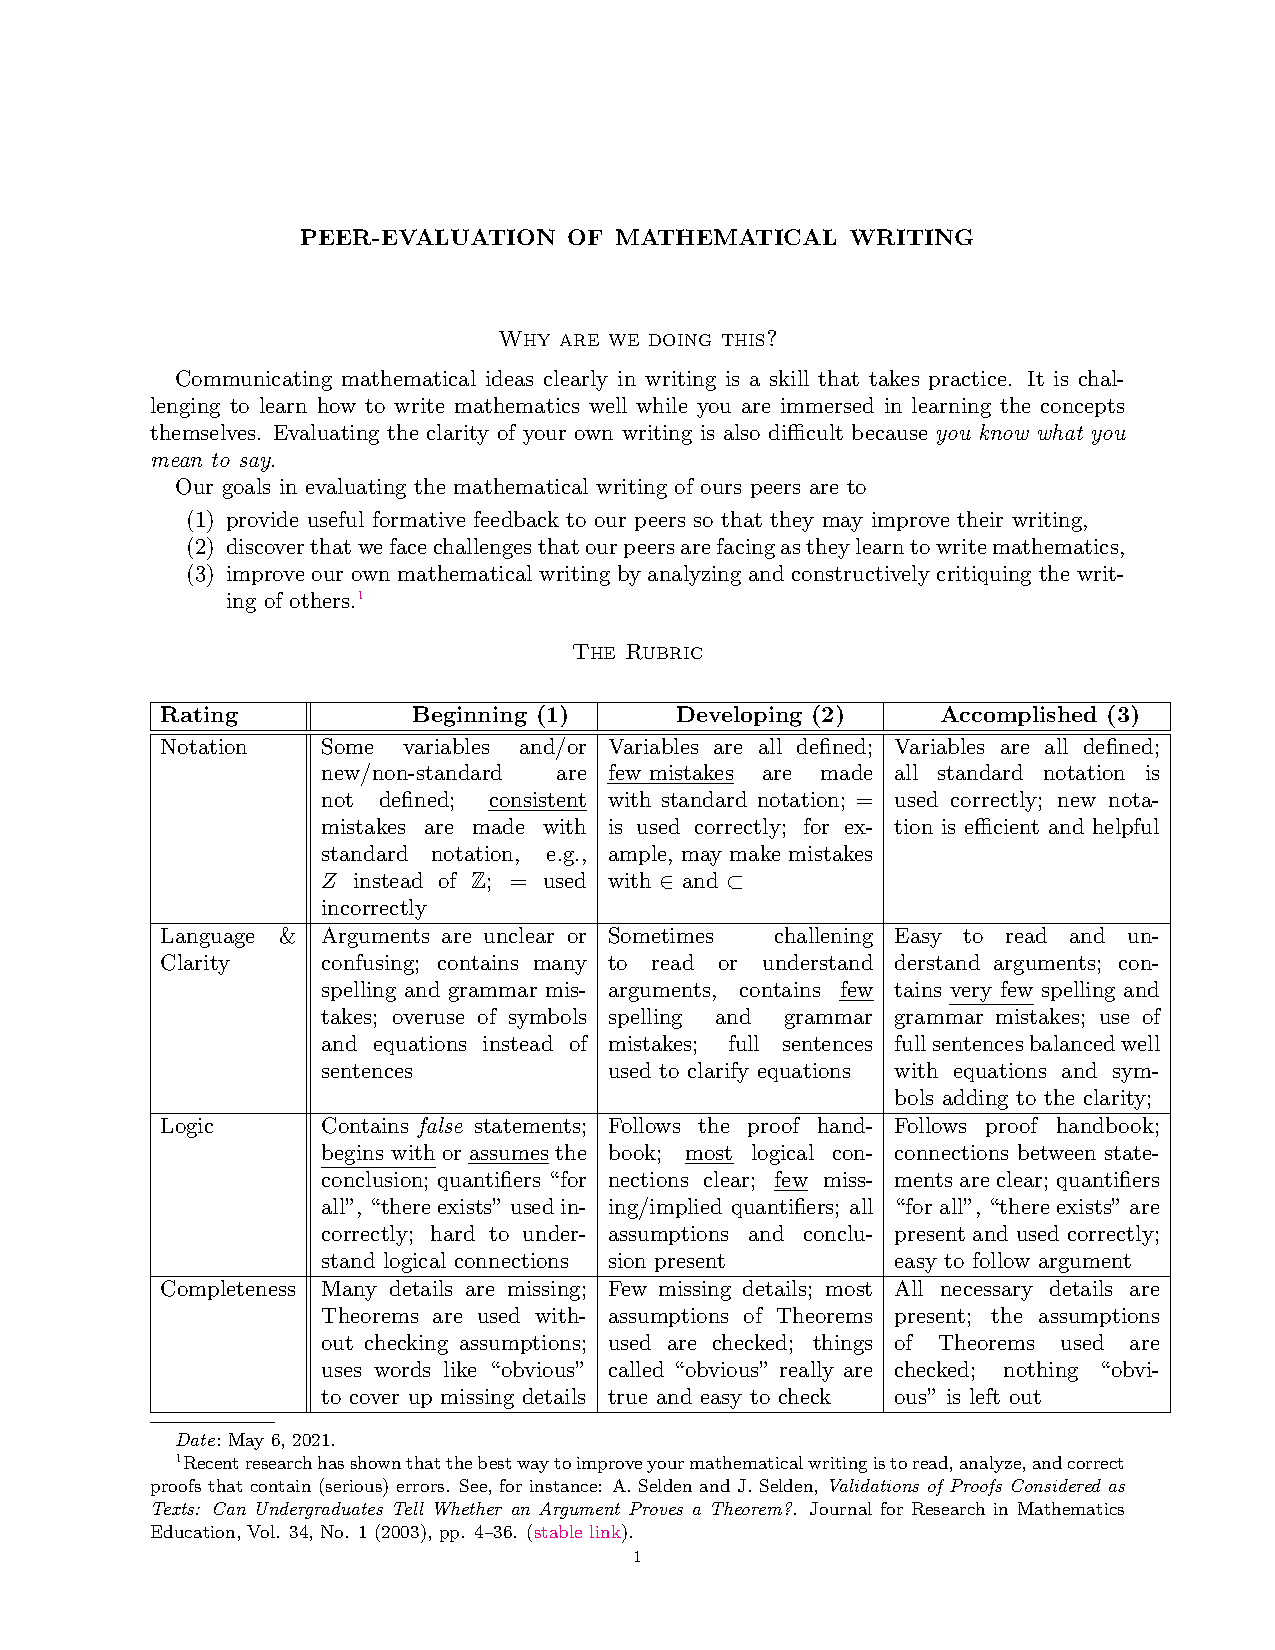
\includepdf[pages=-]{Rubrics/peer-discrete.pdf}
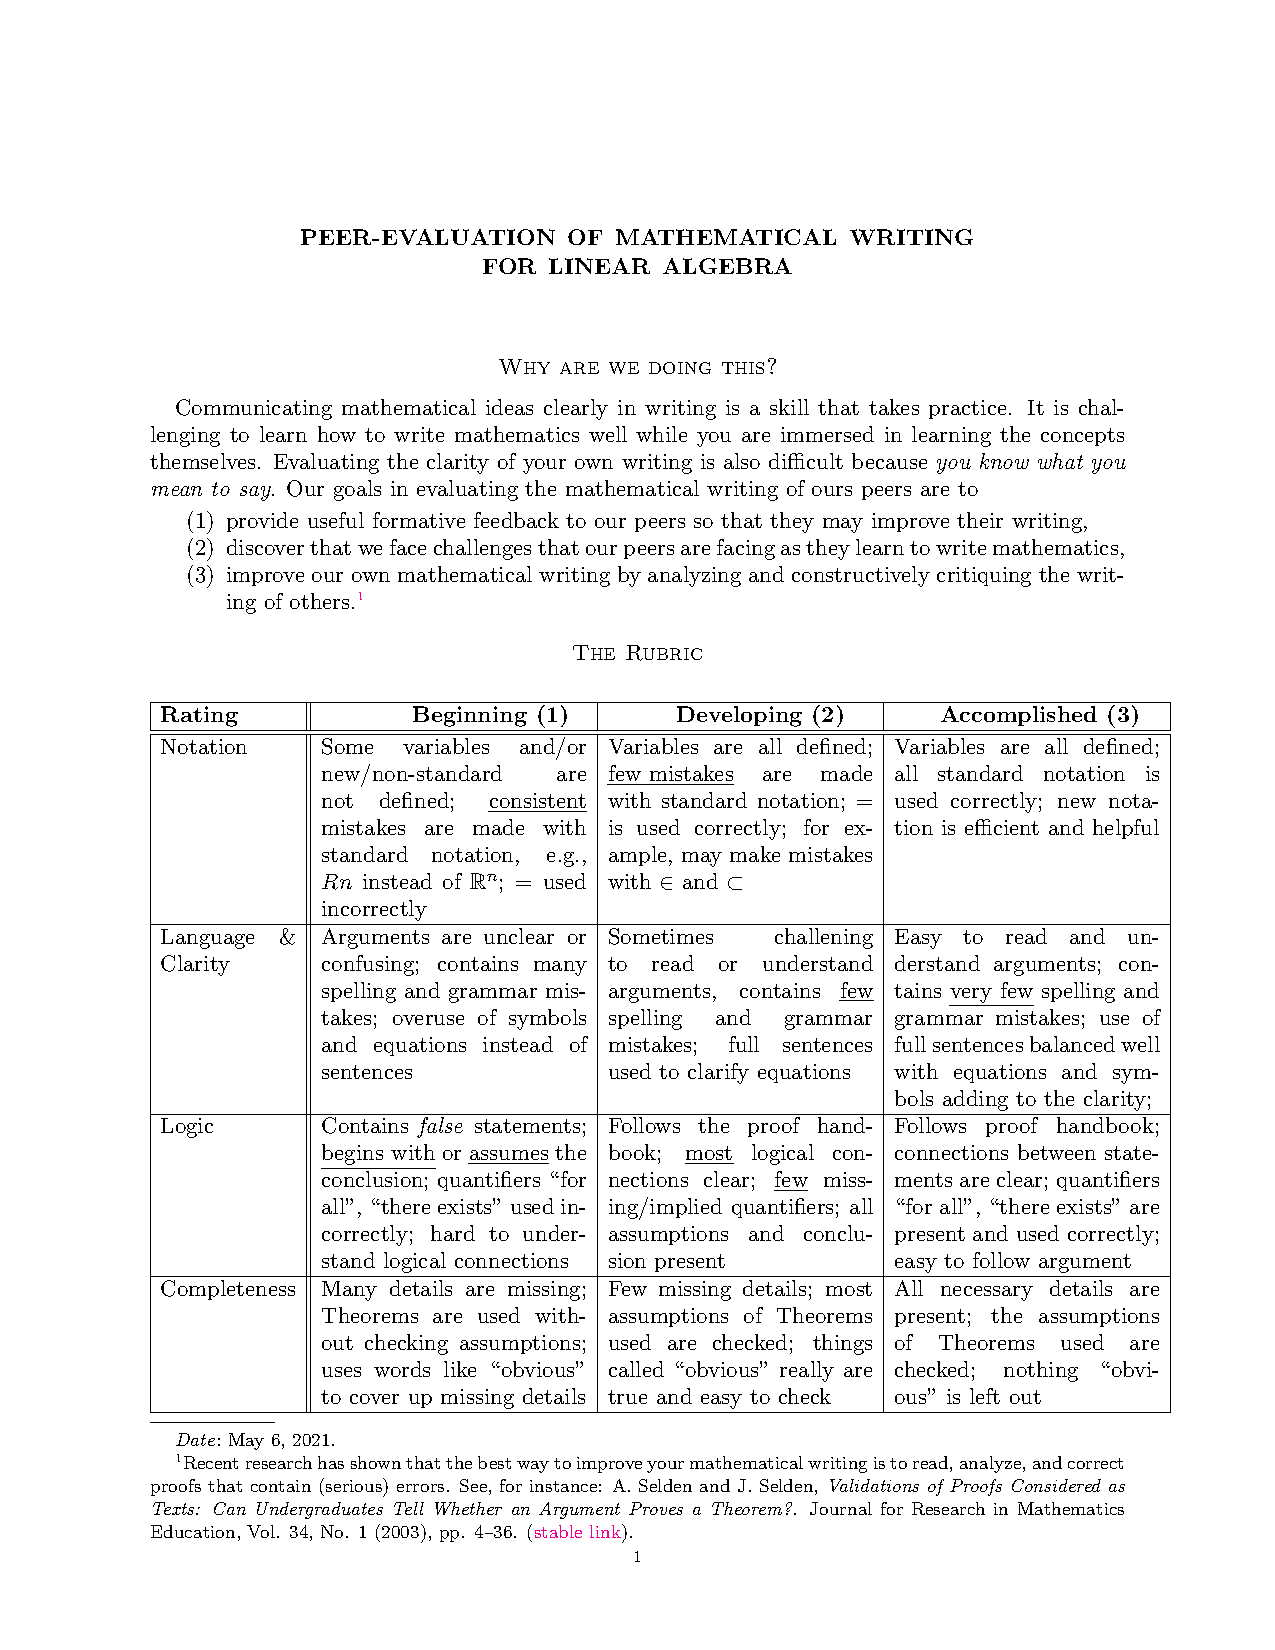
\includepdf[pages=-]{Rubrics/peer-linear.pdf}

%-----------------%-----------------
\section{Summative Rubrics}\label{ch-sum}
%-----------------%-----------------
Here is a sample summative rubric for a linear algebra course. Breaking the rubric into a \emph{Mathematics Score} and a \emph{Communication Score} helps to emphasize that mathematical communication is very important and will contribute to their grade.

In practice, I usually provide this sample rubric to my students as a guide, but then fine-tune it for each individual question. In particular, for each question I break down the \emph{Mathematics Score} into concrete pieces (e.g. 1pt for showing the set is linearly independent, etc.). I grade the \emph{Communication Score} holistically. The clause that the \emph{Communication Score} may not exceed the \emph{Mathematics Score} is included so that students who trivialize the problem (e.g., submits a single sentence that contains no communication errors) do not receive a higher score than students who made several communication errors in the process of making good progress towards the problem. In practice, this clause is meant to be taken as a guideline and is not applied strictly.
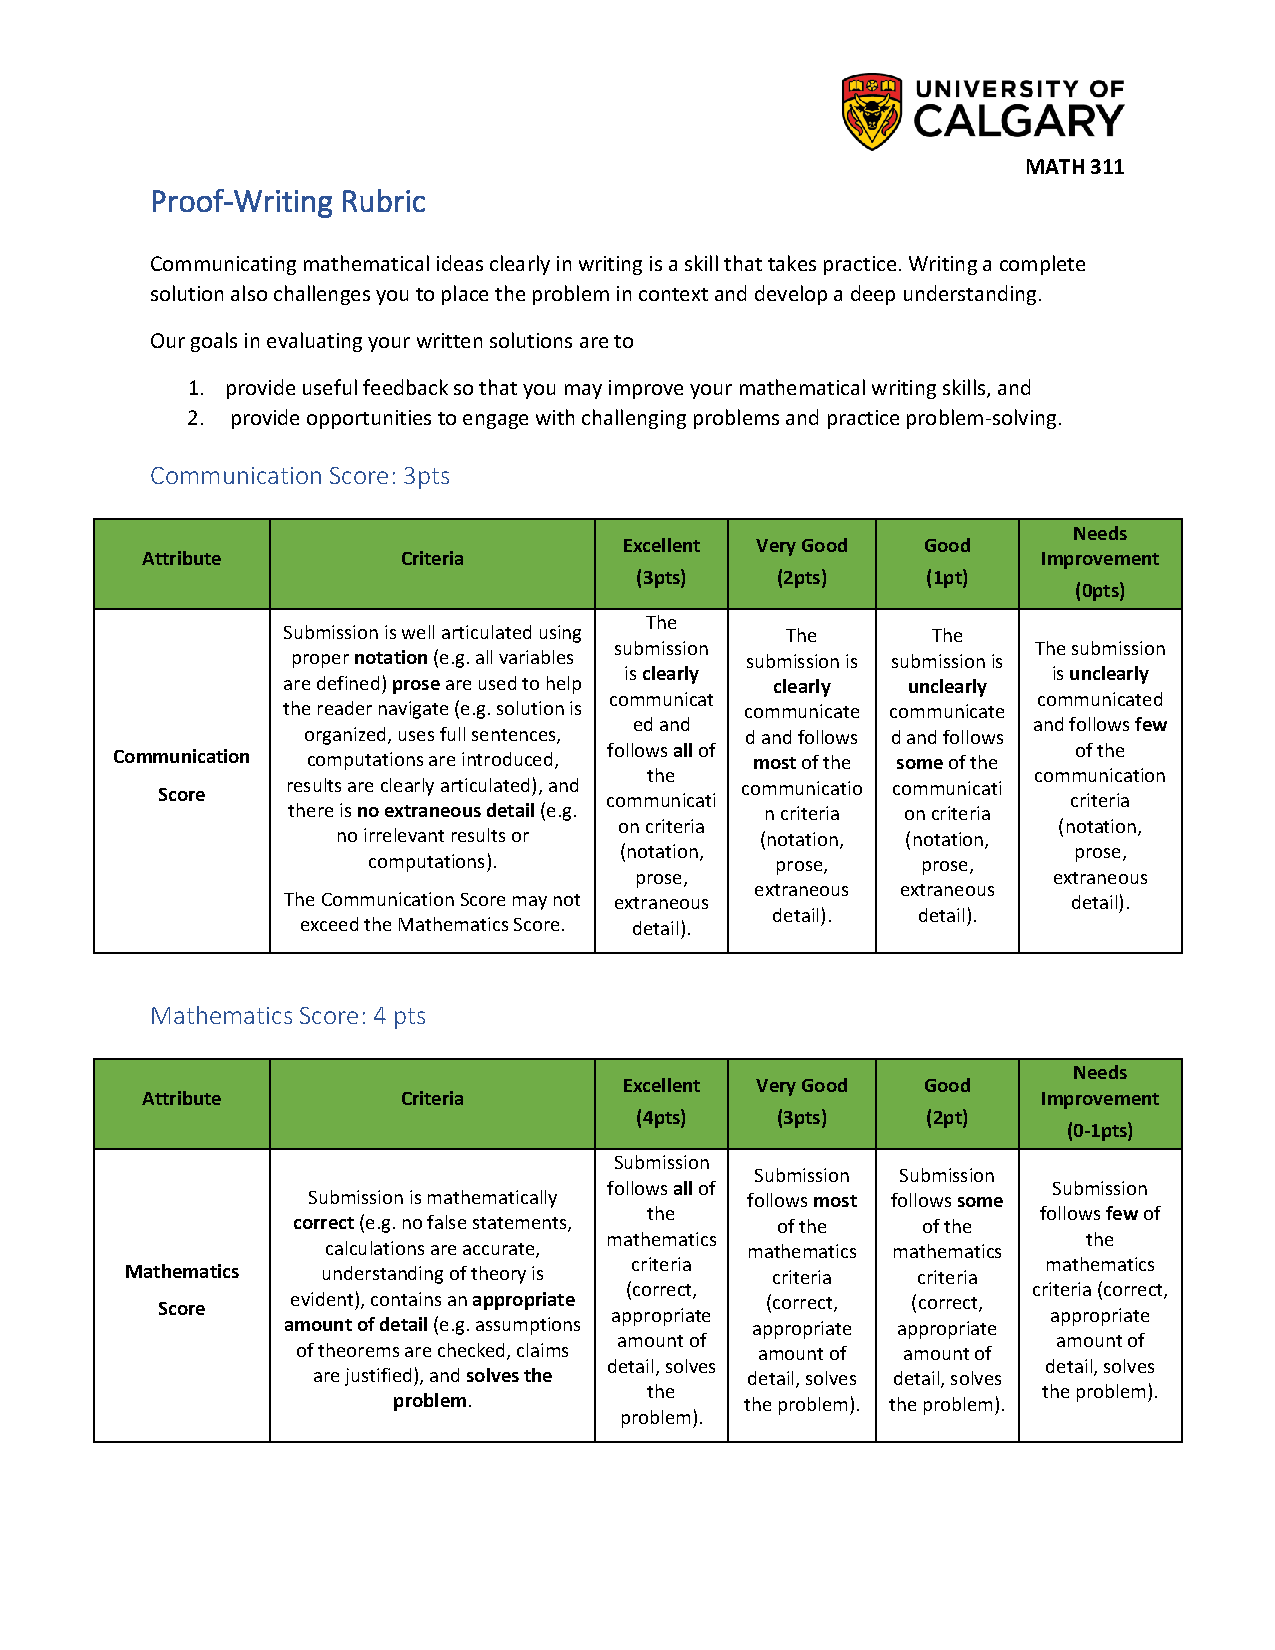
\includepdf[pages=-]{Rubrics/summative-linear.pdf}
%-------------------Bibliography----------------------------
%% ***   Set the bibliography style.   ***
%% (change according to your preference)
\addcontentsline{toc}{chapter}{Bibliography}
\bibliographystyle{amsplain}

%\nocite{*}
%% ***   Set the bibliography file.   ***
\bibliography{sotl}
%-----------------%-----------------
%\appendix
%
%\chapter{``Thi's Bible"}
%The following one-page handout, affectionately known at the University of Calgary as ``Thi's Bible", is designed to help novice proof writers identify exactly \emph{what needs to be done} in order to prove a mathematical statement.  In addition, some fundamental conventions and common errors are highlighted.
%\includepdf[pages=-]{thi-bible.pdf}
%-----------------%-----------------
\end{document}
